% P1: Design and Evaluation of a Drift-Aware Continuous Learning MLOps Framework for Financial Transaction Fraud Detection
% Generated by build_latex.py from content.py. Compiles on Overleaf with pdflatex.
% To use the official BRAC template instead, paste chapters/*.tex and the bibliography there.
\documentclass[12pt,a4paper]{report}
\usepackage[margin=1in]{geometry}
\usepackage[T1]{fontenc}
\usepackage{graphicx,longtable,booktabs,array,enumitem,setspace,amsmath,amssymb}
\usepackage[hidelinks]{hyperref}
\usepackage{url}
\onehalfspacing
\setlist[enumerate]{itemsep=2pt}

\begin{document}
\pagenumbering{gobble}
\begin{titlepage}
\centering
{\LARGE\bfseries Design and Evaluation of a Drift-Aware Continuous Learning MLOps Framework for Financial Transaction Fraud Detection\par}
\vspace{1.5em} by\par\vspace{1em}
Mashud Hasan\\ 22299053\\[0.4em]
Nirnoy Biswas\\ 24241185\\[0.4em]
Md. Sabbir Hossain\\ 22299038\\[0.4em]
Al Imran\\ 231011035\\[0.4em]
Imtiaz Zaman Sami\\ 23101551\par
\vfill
A thesis submitted to the Department of Computer Science and Engineering\\ in partial fulfillment of the requirements for the degree of\\ B.Sc. in Computer Science and Engineering\par
\vspace{1.5em}
Department of Computer Science and Engineering\\ Brac University\\ [Month Year]\par
\vfill
\copyright 2026. Brac University\\ All rights reserved.
\end{titlepage}

\pagenumbering{roman}
\chapter*{Declaration}\addcontentsline{toc}{chapter}{Declaration}
It is hereby declared that
\begin{enumerate}
  \item The thesis submitted is our own original work while completing degree at Brac University.
  \item The thesis does not contain material previously published or written by a third party, except where this is appropriately cited through full and accurate referencing.
  \item The thesis does not contain material which has been accepted, or submitted, for any other degree or diploma at a university or other institution.
  \item We have acknowledged all main sources of help.
\end{enumerate}
\vspace{1em}\noindent\textbf{Student's Full Name \& Signature:}\par
\begin{minipage}[t]{0.45\textwidth}\centering\vspace{2.2em}\rule{0.8\textwidth}{0.4pt}\\ Mashud Hasan\\ 22299053\end{minipage}
\hfill
\begin{minipage}[t]{0.45\textwidth}\centering\vspace{2.2em}\rule{0.8\textwidth}{0.4pt}\\ Nirnoy Biswas\\ 24241185\end{minipage}
\hfill
\begin{minipage}[t]{0.45\textwidth}\centering\vspace{2.2em}\rule{0.8\textwidth}{0.4pt}\\ Md. Sabbir Hossain\\ 22299038\end{minipage}
\hfill
\begin{minipage}[t]{0.45\textwidth}\centering\vspace{2.2em}\rule{0.8\textwidth}{0.4pt}\\ Al Imran\\ 231011035\end{minipage}
\hfill
\begin{minipage}[t]{0.45\textwidth}\centering\vspace{2.2em}\rule{0.8\textwidth}{0.4pt}\\ Imtiaz Zaman Sami\\ 23101551\end{minipage}

\chapter*{Approval}\addcontentsline{toc}{chapter}{Approval}
The thesis titled ``Design and Evaluation of a Drift-Aware Continuous Learning MLOps Framework for Financial Transaction Fraud Detection'' submitted by
\begin{enumerate}
  \item Mashud Hasan (22299053)
  \item Nirnoy Biswas (24241185)
  \item Md. Sabbir Hossain (22299038)
  \item Al Imran (231011035)
  \item Imtiaz Zaman Sami (23101551)
\end{enumerate}
of Spring, 2026 has been accepted as satisfactory in partial fulfillment of the requirement for the degree of B.Sc. in Computer Science and Engineering in Summer 2026.

\vspace{1em}\noindent\textbf{Examining Committee:}\par\vspace{0.5em}
\noindent\begin{minipage}[t]{0.3\textwidth}\textbf{Supervisor:}\\ (Member)\end{minipage}\begin{minipage}[t]{0.65\textwidth}\vspace{1.5em}\rule{0.7\textwidth}{0.4pt}\\ Md. Sabbir Ahmed\\ Senior Lecturer\\ Department of Computer Science and Engineering\\ Brac University\end{minipage}\\[1.5em]
\noindent\begin{minipage}[t]{0.3\textwidth}\textbf{Co-Supervisor:}\\ (Member)\end{minipage}\begin{minipage}[t]{0.65\textwidth}\vspace{1.5em}\rule{0.7\textwidth}{0.4pt}\\ Naima Tahsin Nodi\\ Adjunct Lecturer\\ Department of Computer Science and Engineering\\ Brac University\end{minipage}\\[1.5em]
\noindent\begin{minipage}[t]{0.3\textwidth}\textbf{Thesis Coordinator:}\\ (Member)\end{minipage}\begin{minipage}[t]{0.65\textwidth}\vspace{1.5em}\rule{0.7\textwidth}{0.4pt}\\ Dr. Md. Golam Rabiul Alam\\ Professor\\ Department of Computer Science and Engineering\\ Brac University\end{minipage}\\[1.5em]
\noindent\begin{minipage}[t]{0.3\textwidth}\textbf{Head of Department:}\\ (Chair)\end{minipage}\begin{minipage}[t]{0.65\textwidth}\vspace{1.5em}\rule{0.7\textwidth}{0.4pt}\\ Dr. Sadia Hamid Kazi\\ Chairperson\\ Department of Computer Science and Engineering\\ Brac University\end{minipage}\\[1.5em]

\chapter*{Abstract}\addcontentsline{toc}{chapter}{Abstract}
Machine-learning models for financial transaction fraud detection are usually trained once and evaluated on a random split of historical data. In production this picture breaks down: fraud patterns and customer behaviour change over time (concept drift), and the true label of a transaction becomes known only weeks later, when a chargeback is filed (label delay). MLOps platforms usually decide when to retrain with statistical drift detectors on the input data, but whether such detectors reflect the performance of a fraud model when labels arrive late had not been tested.

This thesis designs and evaluates a drift-aware continuous learning MLOps framework for fraud detection. Here, drift-aware means that the framework tracks drift through the performance of the model on labels as they mature, rather than relying on label-free drift alarms. The framework monitors a LightGBM model on delayed labels, retrains it on a fixed schedule with a performance safety net, selects the training window automatically, and promotes a new model only if a promotion gate confirms that it is at least as good as the live model on unseen data. It is built with MLflow, a FastAPI scoring service and a monitoring dashboard, and is evaluated by replaying three public datasets (IEEE-CIS, Sparkov and Bank Account Fraud) as live streams under label delays of 0 to 60 days, with paired bootstrap confidence intervals, walk-forward tuning, five training seeds, an equal-budget comparison and fault injection.

Drift indicators proved unreliable in both directions: on IEEE-CIS the PR-AUC of a static model fell from 0.58 to 0.39 while the drift of its scores stayed below 0.02, whereas on Sparkov and BAF strong input drift (PSI up to 4.6) caused no loss of performance. Retraining helped on every dataset when its window suited the data, but its benefit on IEEE-CIS fell from +0.078 to +0.010 PR-AUC as the label delay grew to 60 days. Tuned fairly, drift-triggered retraining was reliably worse than scheduled retraining in seven of nine comparisons and never better; with delayed labels the schedule matched or beat it also at an equal number of retrains. Automatic window selection matched the best fixed window on two datasets and came within 0.005 PR-AUC on the third, and the promotion gate blocked every model trained on corrupted data that it could observe.

\noindent\textbf{Keywords:} Financial fraud detection, concept drift, label delay, continuous learning, MLOps, scheduled retraining, promotion gate, LightGBM, PR-AUC

\chapter*{Acknowledgement}\addcontentsline{toc}{chapter}{Acknowledgement}
Firstly, we thank Allah, the Most High, for everything He has bestowed upon us.

We would like to express our sincere gratitude to our supervisor, Md. Sabbir Ahmed sir, and our co-supervisor, Naima Tahsin Nodi ma'am, for their guidance and support throughout this research. Their feedback helped us to sharpen the research question and to overcome the difficulties we faced during the work.

We also thank the IEEE Computational Intelligence Society and Vesta Corporation for releasing the IEEE-CIS Fraud Detection dataset, the maintainers of the Sparkov credit-card dataset, and all the researchers whose articles and open-source tools have shaped this work.

\tableofcontents
\listoffigures\addcontentsline{toc}{chapter}{List of Figures}
\listoftables\addcontentsline{toc}{chapter}{List of Tables}
\chapter*{Nomenclature}\addcontentsline{toc}{chapter}{Nomenclature}
The next list describes several symbols and abbreviations that will be used later within the body of the document.\par\vspace{0.5em}
\noindent\begin{tabular}{@{}p{0.18\textwidth}p{0.75\textwidth}@{}}
\textbf{ADWIN} & Adaptive Windowing (drift detector) \\
\textbf{API} & Application Programming Interface \\
\textbf{CI} & Confidence Interval \\
\textbf{DDM} & Drift Detection Method \\
\textbf{FDS} & Fraud Detection System \\
\textbf{GNN} & Graph Neural Network \\
\textbf{KS} & Kolmogorov-Smirnov (test) \\
\textbf{MLOps} & Machine Learning Operations \\
\textbf{PR-AUC} & Area Under the Precision-Recall Curve \\
\textbf{PSI} & Population Stability Index \\
\textbf{ROC-AUC} & Area Under the Receiver Operating Characteristic Curve \\
\textbf{SHAP} & SHapley Additive exPlanations \\
\textbf{SMOTE} & Synthetic Minority Over-sampling Technique \\
\end{tabular}

\clearpage
\pagenumbering{arabic}
\chapter{Introduction}

\section{Background}

Digital payments have become the default way of paying for goods and services. Card payments, online shopping, mobile banking and cross-border e-commerce now generate millions of transactions every day, and each of them is an opportunity for fraud. Financial crime is estimated to cost U.S. institutions alone more than 32 billion dollars each year \cite{uddin2026}. For banks and payment processors, detecting fraudulent transactions quickly and accurately is therefore both a financial and a trust problem.

Modern fraud detection systems (FDS) combine fixed business rules with machine-learning models that score each transaction and raise alerts for investigators \cite{dalpozzolo2018,alessi2026}. A large body of work has compared classifiers, ensembles and class-imbalance techniques on public data \cite{dang2021,abdelnaby2023,sohony2018,mienye2023}, and gradient boosted trees such as XGBoost have proved to be strong models for tabular fraud data \cite{amekoe2024,uddin2026}. Most of this work, however, studies the model at a single point in time: it is trained on a random sample of historical transactions and tested on another random sample from the same period.

Real systems do not work like that. A model is trained on the past and then used on the future, and the future does not stand still. Customers change their spending habits, merchants and products change, and fraudsters adapt their strategies to whatever the current model does not catch. This change in the relationship between transactions and fraud over time is known as concept drift \cite{pulicharla2019,kodakandla2024}. Under concept drift, a model that performed well at deployment slowly, and sometimes suddenly, becomes less accurate. Menezes and Filho, for example, found that the F1-score of graph neural network fraud detectors trained on the IEEE-CIS dataset fell by up to 40\% over the following weeks \cite{menezes2025}.

Fraud detection adds a second difficulty that most drift research does not consider: the true label of a transaction is not known when the model makes its decision. A fraud is usually confirmed only when the cardholder notices it and files a chargeback, and a legitimate transaction is only confirmed when the dispute window has passed. Dal Pozzolo et al. call this verification latency and show that it strongly affects how a fraud model can be updated \cite{dalpozzolo2018}, and Amekoe et al. showed that it changes which learning strategies work best \cite{amekoe2024}. In practice, the labels a system can learn from are often weeks old, which means that it can only notice that its performance has dropped long after the drop has happened.

Machine Learning Operations (MLOps) has emerged to handle exactly this kind of problem: keeping machine-learning models reliable after deployment through automated pipelines for training, versioning, monitoring and redeployment \cite{pulicharla2019,kodakandla2024}. A central MLOps practice is continuous training, where models are retrained either on a fixed schedule or when a monitoring signal indicates that the data has drifted \cite{pulicharla2019}. Recent research increasingly favours the second option, triggering retraining when statistical drift measures such as the Population Stability Index (PSI) or the Kolmogorov-Smirnov (KS) test exceed a threshold \cite{shakil2025,wong2025}. Whether such triggers actually track the performance of a fraud model when labels arrive late is, however, an open question. This thesis addresses that question and builds a framework around the answer.

In this thesis, a \textit{drift-aware} system is one that is aware of drift through its effect on the model: it tracks the performance of the deployed model on labels as they mature, and treats label-free drift measures as diagnostic information rather than as a reason to retrain. As the results will show, this distinction matters, because drift indicators alone can both miss real degradation and raise alarms about drift that does no harm.

\section{Motivation}

The first motivation for this study is the gap between how fraud models are evaluated in research and how they are used in practice. Many studies report near-perfect results on public credit-card datasets using random train-test splits and synthetic oversampling \cite{mienye2023}. Dang et al. showed that such results can be inflated when resampling is applied before splitting \cite{dang2021}, and a random split has a similar effect in time: the model is tested on transactions from the same period it was trained on, so concept drift is invisible. A fraud model that will be deployed on future transactions must be evaluated on future transactions.

The second motivation is that the decision of when to retrain a model is costly in both directions. Retraining too rarely leaves a degraded model in service and lets fraud through. Retraining too often wastes computing resources and, more importantly, increases the chance of deploying a bad model, for example one trained on incomplete or corrupted data. MLOps systems therefore need a policy that decides when retraining is actually necessary and a safeguard that decides whether a newly trained model may replace the one in service.

The third motivation is that recent work proposing drift-triggered retraining has been evaluated under conditions that favour it. Shakil et al. proposed a feature-drift indicator to decide when retraining is warranted, but tested it on drift that was artificially induced into non-fraud datasets \cite{shakil2025}. Wong and Perumal reported that an agentic, drift-triggered retraining scheduler outperformed weekly retraining, but on a single industrial dataset with injected drift \cite{wong2025}. Yelleti retrained fraud models only when a drift detector fired, but assumed that labels arrive immediately \cite{yelleti2025}. Shakil et al. themselves note that statistical drift does not always correspond to a change in model performance \cite{shakil2025}.

Finally, we are motivated by our own preliminary experiments on the IEEE-CIS dataset, which already challenge the common assumption. A LightGBM model trained once lost about a third of its weekly PR-AUC over the following months, yet the drift of its prediction scores stayed far below the usual alarm level, and only one of its ten most important features drifted noticeably. On a second dataset, Sparkov, we observed the opposite: strong input drift with almost no loss of accuracy. If drift detectors can both miss real decay and raise false alarms, a drift-aware system has to be designed around what drift detection can and cannot see. This is the perspective this thesis takes.

\section{Problem Statement}

We consider a fraud detection model deployed on a continuous stream of card transactions. Each transaction must be scored immediately, but its fraud label becomes available only after a label delay of several days to several weeks. Over time the distribution of transactions and the relationship between transaction features and fraud change. The operator of the system must decide, at regular intervals, whether to retrain the model, which data to retrain it on, and whether the retrained model is safe to put into service.

Existing approaches leave several parts of this problem unresolved:

\begin{enumerate}
  \item \textbf{Unrealistic evaluation.} Most fraud studies use random splits of static data, so they cannot show how performance evolves after deployment or how much retraining helps \cite{abdelnaby2023,mienye2023}.
  \item \textbf{Unverified retraining triggers.} Label-free drift measures such as PSI and KS are widely used to trigger retraining, but whether they track the performance of a fraud model has not been established on real, naturally drifting data \cite{shakil2025,wong2025}.
  \item \textbf{Ignored label delay.} Most retraining studies assume that labels are available immediately, although verification latency is a defining property of fraud detection \cite{dalpozzolo2018,amekoe2024}.
  \item \textbf{No fair comparison of retraining policies.} Scheduled and drift-triggered retraining are rarely compared under the same conditions, with tuned settings, uncertainty estimates and realistic label delay.
  \item \textbf{Unsafe model updates.} Automated retraining can deploy a model trained on corrupted labels or features; few frameworks test whether their safeguards actually stop such models.
  \item \textbf{Limited reproducibility.} Studies with realistic operating conditions often rely on private bank data \cite{dalpozzolo2018,somasundaram2019,aldaoud2025}.
\end{enumerate}

This thesis addresses these gaps through the following research questions:

\begin{itemize}[label={}, leftmargin=2em]
  \item \textbf{RQ1:} How does the performance of a fraud detection model evolve after deployment, and do label-free drift measures reflect that change?
  \item \textbf{RQ2:} How much does retraining improve performance, and how does label delay change that benefit?
  \item \textbf{RQ3:} Does drift-triggered retraining outperform scheduled retraining when both are tuned fairly and evaluated with realistic label delay?
  \item \textbf{RQ4:} Can an MLOps framework built on these findings sustain performance on a live stream and prevent faulty models from reaching production?
\end{itemize}

\section{Objective}

The aim of this research is to design and evaluate a drift-aware continuous learning MLOps framework for financial transaction fraud detection that can identify when a deployed model is becoming outdated, decide when retraining is actually necessary, and safely deploy a better retrained model without unnecessary retraining. The specific objectives are:

\begin{enumerate}
  \item To review existing research on fraud detection, concept drift, label delay, retraining strategies and MLOps, and identify the gaps this thesis addresses.
  \item To prepare three public fraud datasets, IEEE-CIS, Sparkov and BAF, for strictly time-ordered evaluation, without leakage from future transactions.
  \item To measure how a model trained once degrades over time, and whether label-free drift measures (PSI of features and of model scores) track that degradation.
  \item To simulate retraining strategies under label delays of 0 to 60 days: a static model, scheduled retraining on all past data or on a sliding window, and retraining triggered by drift in scores or by a drop in delayed-label performance.
  \item To compare these strategies with paired day-block bootstrap confidence intervals, walk-forward tuning of their settings and repeated training seeds.
  \item To implement an MLOps framework with delayed-label monitoring, a retraining policy, a promotion gate, a model registry, a scoring service and a monitoring dashboard.
  \item To test the safeguards of the framework by injecting realistic faults (corrupted labels, a chargeback outage and a feature unit bug) into its retraining jobs.
  \item To check whether the findings generalise by replicating the key experiments on the other two datasets.
\end{enumerate}

\section{Methodology in Brief}

The study follows the workflow shown in Figure \ref{fig:method}. It begins with a review of the literature on fraud detection, concept drift and MLOps, which identifies the gaps listed in the problem statement. Two public datasets are then prepared. IEEE-CIS, released by the IEEE Computational Intelligence Society and Vesta Corporation, contains 590,540 real e-commerce transactions over 182 days with a fraud rate of 3.5\% and has been used in recent drift and fraud studies \cite{menezes2025,uddin2026}. Sparkov contains about 1.8 million simulated card transactions over two years with a fraud rate of 0.5\%. Both are sorted by time and used without any random shuffling; per-card behaviour features for Sparkov are computed only from each card's earlier transactions, so that no information from the future leaks into the model.

\begin{figure}[htbp]
  \centering
  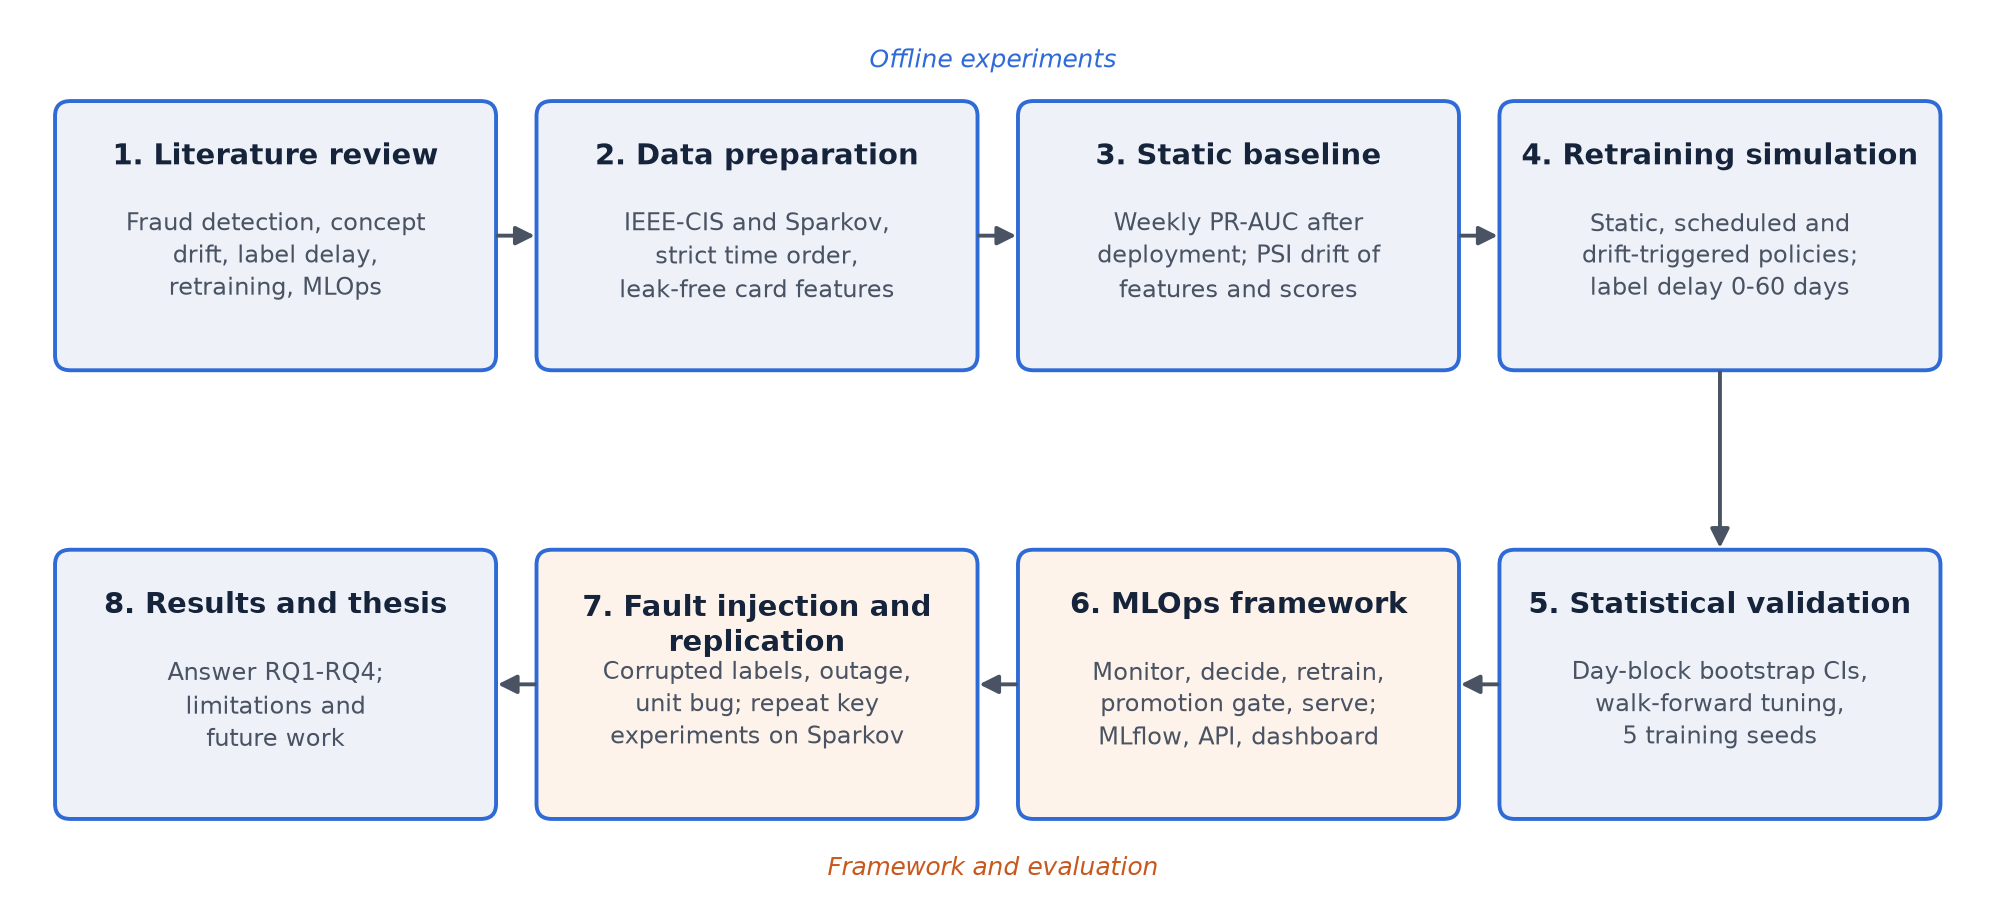
\includegraphics[width=\textwidth]{figures/methodology.png}
  \caption{Methodology of the study: from literature review and time-ordered data preparation to the retraining experiments, the framework and its evaluation}
  \label{fig:method}
\end{figure}

A LightGBM gradient boosted tree model is used throughout, because batch-trained boosted trees are strong, widely used models for tabular fraud data and remain competitive with incremental learners when labels are delayed \cite{amekoe2024}. The study first trains a static model and measures its weekly performance and the PSI drift of its features and scores over the following months. It then replays the later part of each dataset as a stream, week by week, and simulates the retraining strategies listed in the objectives, making labels available only after a chosen delay. PR-AUC is the main metric because fraud is rare and the precision of alerts matters most \cite{dalpozzolo2018}; results are averaged per week so that scores from different model versions are never pooled. Uncertainty is estimated with a paired bootstrap that resamples whole days, strategy settings are tuned walk-forward using only information available at the time, and the key comparisons are repeated with five training seeds.

The findings are then turned into a working framework, shown in Figure \ref{fig:loop}. Every week it measures the live model on labels that have become available, decides whether to retrain, trains a new model on a sliding window of recent labelled data, and promotes it only if a promotion gate confirms that it performs at least as well as the live model on data neither has seen. Models are versioned in MLflow, served through a FastAPI scoring service and tracked on a monitoring dashboard, following common MLOps practice \cite{pulicharla2019}. The framework is evaluated by replaying the stream end to end and by injecting faults into selected retraining jobs to test whether the promotion gate and performance safety net stop faulty models.

\begin{figure}[htbp]
  \centering
  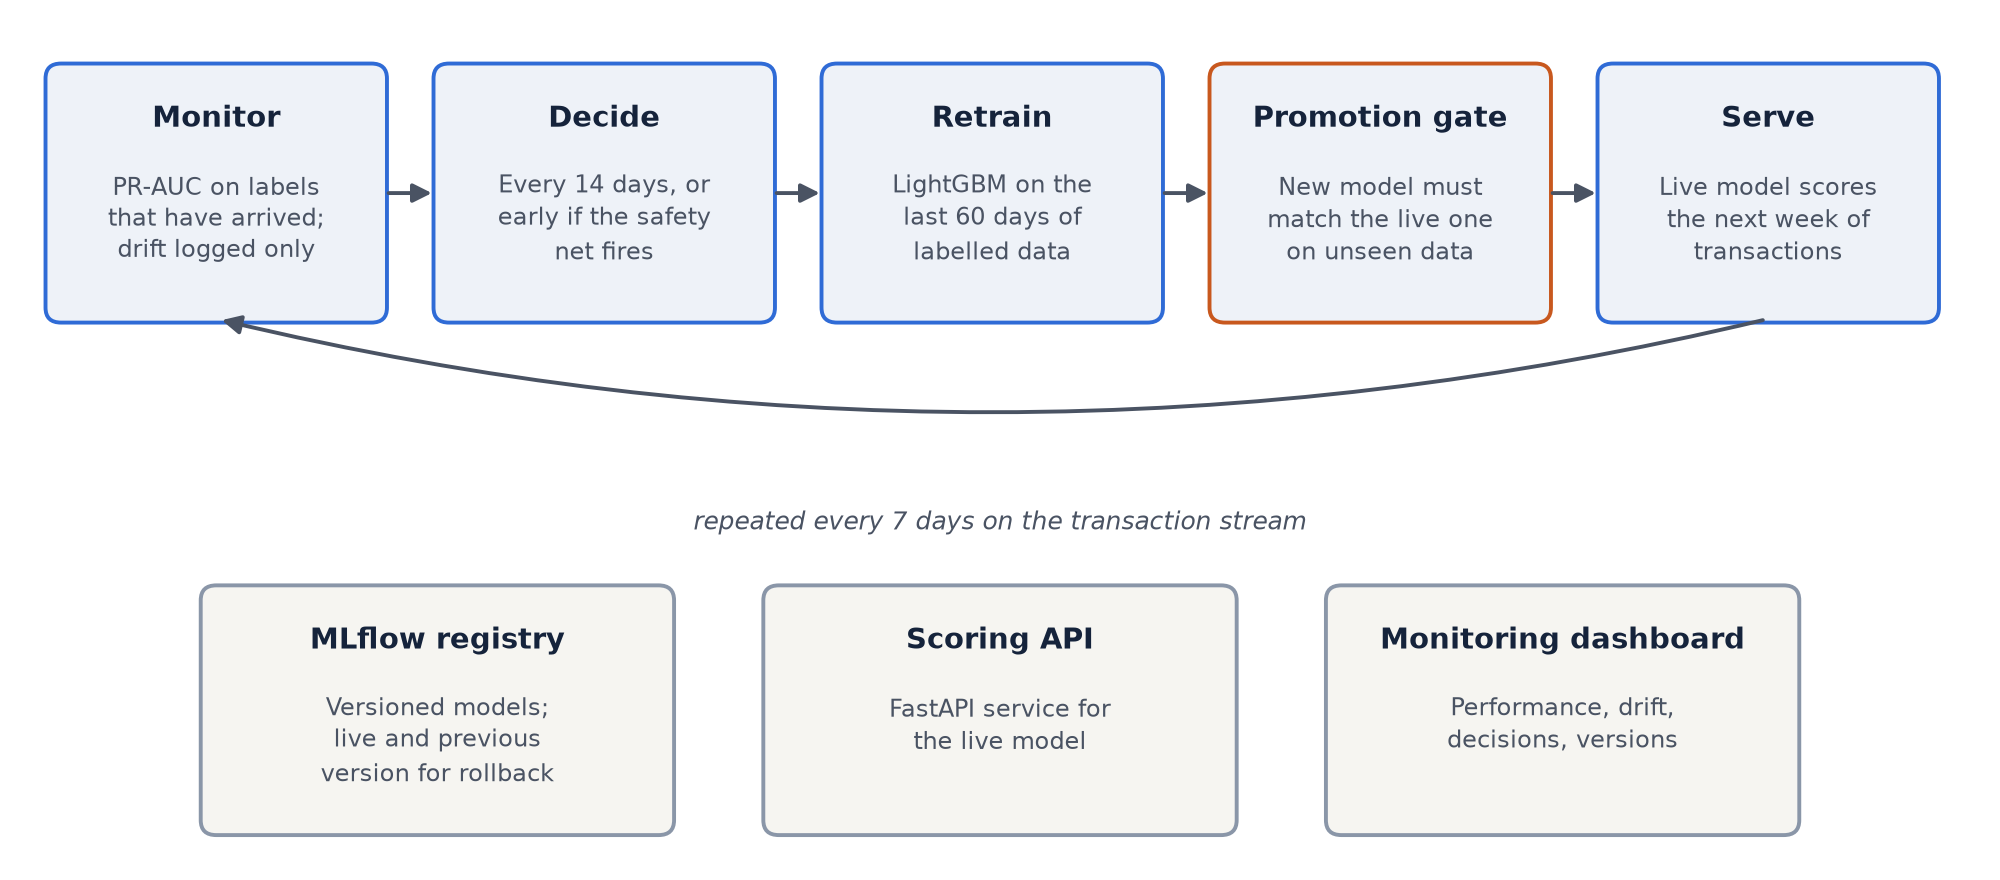
\includegraphics[width=\textwidth]{figures/framework_loop.png}
  \caption{The proposed continuous-learning loop, run every week on the transaction stream}
  \label{fig:loop}
\end{figure}

The experiments were run on IEEE-CIS and repeated on Sparkov and on the Bank Account Fraud (BAF) dataset. They show that drift indicators can miss real degradation under delayed labels, that a fixed retraining schedule is more reliable than drift-triggered retraining when labels are delayed, also at an equal retraining budget, and that the framework reproduces the offline results when replayed. The details are given in Chapters 4 and 5.

\section{Scopes and Challenges}

The study focuses on binary fraud detection for card transactions, where each transaction is scored as fraudulent or legitimate. Its scope is the post-deployment life of a model: how it degrades, when retraining is actually necessary, and how model updates can be made safe. It does not aim to find the best possible classifier, and it does not connect to a real bank or process real customer data. The main areas covered are:

\begin{enumerate}
  \item Time-ordered evaluation of fraud models on two public datasets.
  \item Analysis of performance decay and of label-free drift measures after deployment.
  \item Comparison of static, scheduled and drift-triggered retraining under label delay.
  \item Statistical validation with bootstrap confidence intervals, walk-forward tuning and repeated seeds.
  \item An MLOps framework with monitoring, retraining policy, promotion gate, model registry, scoring service and dashboard.
  \item Fault-injection testing of the framework's safeguards.
\end{enumerate}

The study also faces several challenges:

\begin{enumerate}
  \item \textbf{Label delay:} performance can only be measured on labels that have matured, so problems are always detected late.
  \item \textbf{Class imbalance:} frauds are rare (0.5\% to 3.5\% of transactions), which makes weekly performance estimates noisy and requires careful statistics.
  \item \textbf{Simulated deployment:} the stream is replayed from historical data, so live latency and real label-feed behaviour are not observed.
  \item \textbf{Limited datasets:} public fraud data with timestamps is scarce; IEEE-CIS covers only six months and Sparkov is simulated.
  \item \textbf{Anonymised features:} many IEEE-CIS features are masked, which limits the interpretation of which features drift and why.
  \item \textbf{Computational cost:} repeated retraining over long streams, several label delays and many policy settings requires hours of computation per experiment.
  \item \textbf{Generalisation:} results obtained with one model family and two datasets may not transfer to every institution or fraud type.
\end{enumerate}

Despite these challenges, the study can provide practical, evidence-based guidance on how fraud detection models should be maintained after deployment, and a reproducible open framework that implements it.

\chapter{Literature Review}

\section{Preliminaries}

\textbf{Fraud detection as a learning problem.} Transaction fraud detection is a binary classification task on a continuous stream of transactions. Frauds are rare, typically well under 5\% of transactions, so the task is highly imbalanced and accuracy is a misleading measure \cite{abdelnaby2023,aldaoud2025}. Precision and recall of the fraud class, and summary measures such as PR-AUC, describe performance more faithfully. In an operational FDS, investigators can only check a limited number of alerts per day, so the precision of the top-ranked alerts matters most \cite{dalpozzolo2018}.

\textbf{Concept drift.} Model drift is the loss of performance that follows when deployed data no longer resembles the training data \cite{pulicharla2019}. It takes several forms: \textit{concept drift}, where the relationship between features and labels changes; \textit{covariate shift}, where the distribution of the input features changes; and \textit{label drift}, where the frequency of the classes changes \cite{pulicharla2019,kodakandla2024}. Only a change in the relationship between features and labels necessarily harms a model; a change in the inputs may or may not. Drift can also be described by how it unfolds, as illustrated in Figure \ref{fig:drift}. In \textit{sudden} drift the old pattern is replaced at once; in \textit{gradual} drift the old and new patterns alternate, with the new one becoming more frequent; in \textit{incremental} drift the pattern moves slowly through intermediate states; and in \textit{recurring} drift earlier patterns return, for example with seasonal spending. Fraud is an adversarial setting, so drift is frequent, irregular and partly caused by the detection system itself \cite{menezes2025,hassan2026}.

\begin{figure}[htbp]
  \centering
  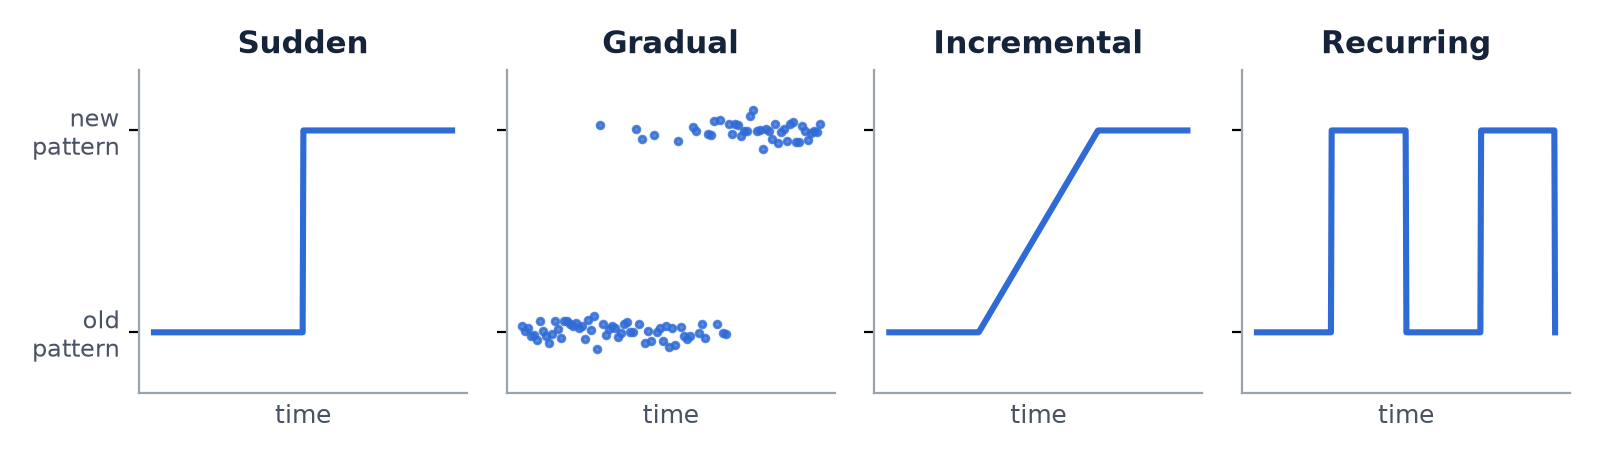
\includegraphics[width=\textwidth]{figures/drift_types.png}
  \caption{Types of concept drift by how the underlying fraud pattern changes over time}
  \label{fig:drift}
\end{figure}

\textbf{Drift detection.} Drift detectors fall into two broad groups. Label-free detectors compare the distribution of recent inputs or model scores with a reference, using measures such as the PSI, the KS test or the Kullback-Leibler divergence \cite{shakil2025,wong2025}; they can run immediately but only see changes in the inputs or the scores. The PSI is commonly read as stable below 0.1, moderately shifted between 0.1 and 0.25, and strongly shifted above 0.25, and Wong and Perumal used 0.25 as their retraining threshold \cite{wong2025}. Error-based detectors such as DDM, EDDM and ADWIN monitor the model's error rate and signal drift when it rises \cite{yelleti2025,aldaoud2025}; they detect real drift but need labels, which in fraud detection arrive late.

\textbf{Verification latency.} In a real FDS, most transactions are labelled only after a delay, when a fraud is reported or when the dispute period ends. A small number of alerted transactions receive quick feedback from investigators. Dal Pozzolo et al. formalised this as verification latency and the alert-feedback interaction, and showed that it changes which data a model can learn from and when \cite{dalpozzolo2018}. Figure \ref{fig:delay} shows the consequence for an automated system. At any moment, the most recent weeks of transactions have already been scored but not yet labelled. Performance can therefore only be measured on older, matured transactions, and a retrained model can only learn from data that ends one label delay before the present. The longer the delay, the later a performance drop is noticed and the older the data a new model is trained on.

\begin{figure}[htbp]
  \centering
  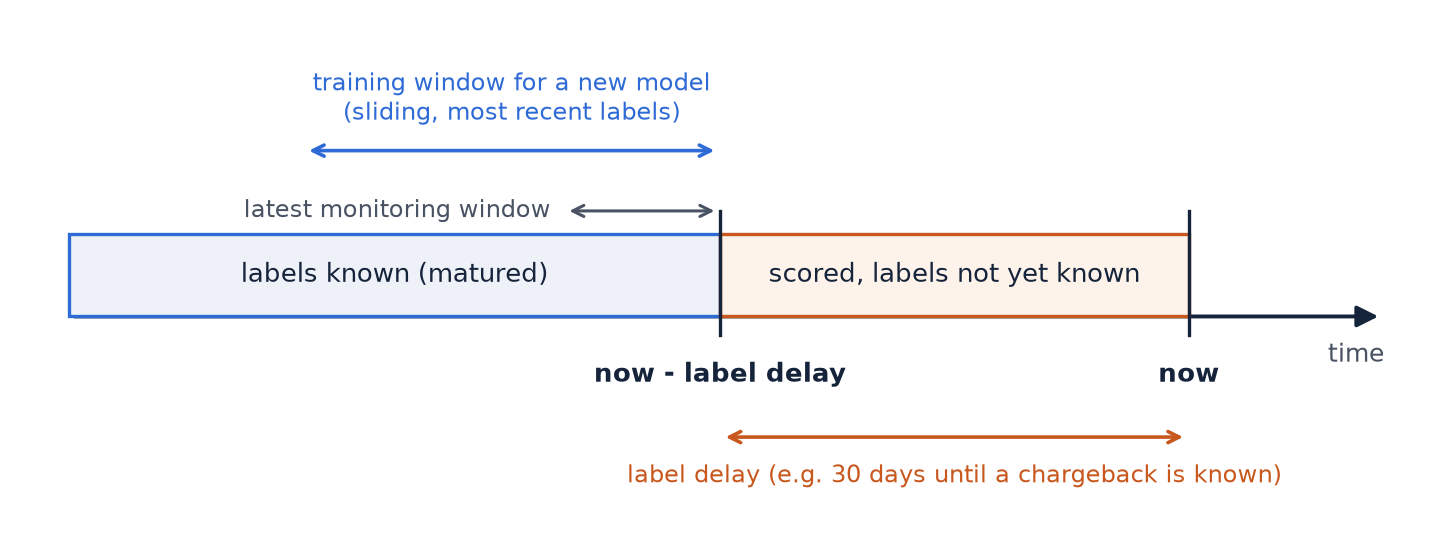
\includegraphics[width=\textwidth]{figures/label_delay.png}
  \caption{Label delay in a fraud detection system: transactions are scored immediately, but their labels become usable only after the delay, which limits both monitoring and retraining}
  \label{fig:delay}
\end{figure}

\textbf{Adaptation strategies.} A deployed model can be kept up to date in several ways. \textit{Periodic} or scheduled retraining rebuilds the model at fixed intervals, while \textit{event-driven} or triggered retraining rebuilds it when a monitoring signal crosses a threshold \cite{pulicharla2019}. The training data may be all history (an expanding window) or only recent data (a sliding window), which forgets outdated patterns \cite{dalpozzolo2018}. \textit{Incremental} or online learning updates the model with every new labelled transaction, and \textit{ensemble} methods combine models trained on different periods \cite{somasundaram2019,yelleti2025}. Which of these works best depends on how quickly labels arrive: under label delay, batch learning can match or beat instance-incremental learning \cite{amekoe2024}.

\textbf{MLOps.} MLOps applies software-engineering practice to the machine-learning lifecycle: automated training pipelines, experiment tracking, versioned model registries, continuous integration and delivery, and monitoring in production \cite{pulicharla2019,kodakandla2024}. Tools such as MLflow, Kubeflow and Apache Airflow automate retraining, while Prometheus, Grafana and Evidently AI support monitoring \cite{pulicharla2019}. Recent MLOps frameworks close the loop between monitoring and retraining for specific domains, such as phishing detection \cite{reda2025} and industrial prediction \cite{wong2025}. A common deployment pattern keeps the model in service (the champion) and promotes a newly trained candidate (the challenger) only if it passes an evaluation, which is the idea behind the promotion gate used in this thesis.

\textbf{Explainability under drift.} Financial regulators expect model decisions to be transparent and auditable, so fraud and credit models are increasingly paired with explanation methods such as SHAP \cite{uddin2026,alessi2026}. Drift affects these explanations too: explanations computed against an outdated reference population can become unstable or unfair as the population changes \cite{john2025}.

\textbf{Evaluation over time.} Evaluating a drifting system requires respecting time: models may only be trained on data from before the period they are tested on \cite{menezes2025}. Common designs include a single chronological split, rolling or walk-forward evaluation, and replaying a historical stream. Because consecutive transactions are correlated, uncertainty estimates should resample whole blocks of time rather than individual transactions.

\section{Review of Existing Research}

\textbf{Fraud detection under drift and label delay.} Dal Pozzolo et al. \cite{dalpozzolo2018} provided one of the most realistic models of a credit-card fraud detection system. Working with an industrial partner and more than 75 million e-commerce transactions collected over three years, they described the layers of an FDS, from terminal checks and blocking rules to the data-driven model and human investigators. They formalised verification latency and the alert-feedback interaction, argued that alert precision is the most meaningful performance measure, and proposed training separate classifiers on recent investigator feedback and on delayed labels, then aggregating their outputs. Their experiments showed that giving more weight to recent feedback produced more precise alerts, and that sliding-window and ensemble approaches handled drift. The work is the foundation for treating label delay as a first-class concern. Its limitations for this thesis are that the data is private, that the timing of retraining is not studied, and that the model is not embedded in an MLOps workflow with monitoring and safe deployment.

Amekoe et al. \cite{amekoe2024} compared instance-incremental learning with batch learning for fraud detection when labels arrive with a delay. Instance-incremental algorithms are usually preferred for evolving streams, but they assume that each label is available immediately. Using fraud detection data and generated datasets, the authors found that instance-incremental learning, including the Adaptive Random Forest, was not the superior option compared with batch-trained models such as XGBoost, and that batch solutions are also easier to interpret. This finding directly supports the design choice of this thesis to retrain a batch model on windows of delayed labels. The study compares learning paradigms, however, and does not examine when to retrain or how to deploy a new model safely.

Yelleti \cite{yelleti2025} proposed ROSFD, a two-stage framework for online streaming fraud detection. An initial model is built offline with incremental learning to avoid a cold start, and in production the drift detectors DDM, EDDM and ADWIN decide when the model is retrained incrementally. Across five datasets, ADWIN gave the best results among the detectors and the Adaptive Random Forest achieved the highest AUC on four of them, while the train-only-when-required strategy substantially reduced how often the model was retrained without a large loss of AUC. The study is close to the question of this thesis, since it tests retraining only when needed. It reports ROC-AUC, which is less informative than PR-AUC for rare fraud, and it assumes labels are available immediately, which makes error-based detectors look more responsive than they would be in practice.

Somasundaram and Reddy \cite{somasundaram2019} proposed a parallel and incremental fraud detection model, Transaction Window Bagging, which combines parallel bagging, incremental learning, cost-sensitive learning and weighted voting to handle concept drift and class imbalance together. Evaluated on Brazilian bank data, it improved the fraud detection rate and the misclassification cost compared with other models. The study is valuable because it treats fraud detection as a continuous stream rather than a static dataset. However, the data is private, label delay is not modelled, and the effect of retraining frequency is not isolated.

Al-Daoud and Abu-AlSondos \cite{aldaoud2025} proposed a hybrid machine-learning framework for fraud detection in Gulf Cooperation Council banks that addresses class imbalance (SMOTEBoost and cost-sensitive learning), adversarial attacks (adversarial training and a FraudGAN), concept drift (DDM and ADWIN) and explainability (SHAP, LIME and human-in-the-loop review). On real bank transactions, the framework raised fraud recall from 35\% to 85\%, reduced the success rate of adversarial attacks from 35\% to 5\%, and recovered from drift within 24 hours while keeping latency below 150 milliseconds. The study shows that drift handling must work together with the other demands of a production fraud system. Drift, however, is one component among many, the retraining policy is not compared with alternatives, and the private data prevents replication.

Alessi and Fugini \cite{alessi2026} developed a real-time financial fraud detection system for transaction data streams that addresses extreme class imbalance and concept drift. It uses a lightweight data stream management system for real-time feature engineering, combines deterministic rules with adaptive machine-learning models, manages the decision threshold dynamically to balance precision and recall, and compares several adaptive learning strategies. It also introduces an interpretability framework that turns low-level feature attributions into concepts investigators can act on. The work demonstrates a practical, operational view of adaptive fraud detection, but it does not test safeguards against faulty model updates or evaluate the effect of label delay on the retraining decision.

Menezes and Filho \cite{menezes2025} studied how graph neural network fraud detectors degrade under natural data drift. They built a heterogeneous knowledge graph from 284,000 IEEE-CIS transactions, trained R-GCN, HGT and HAN models on the earliest 70\%, and then froze the models and monitored them over 50 subsequent 12-hour windows. All models degraded in a volatile, non-monotonic way; the F1-score of HGT fell from 0.747 to as low as 0.455, while the simpler R-GCN was the most stable. They also observed that AUC stayed stable while F1 fluctuated, suggesting that score distributions shift and fixed decision thresholds become outdated. The study is directly relevant because it uses the same dataset and confirms that drift is a real problem on it. However, it only measures degradation: no retraining strategy is evaluated, label delay is not modelled, and the proposed mitigation framework is conceptual.

Hassan \cite{hassan2026} proposed DriftGuard-TriAudit, a concept-drift-aware continual learning framework for financial statement fraud that jointly analyses financial ratios, management discussion text and document layout. It adds modality-specific drift monitoring, reliability-weighted fusion of the three modalities, and memory-based continual learning. On a synthetic benchmark with four temporal fraud scenarios, it achieved an average precision of 0.628 and improved precision over standard continual fine-tuning (0.547 against 0.428) with a similar AUC. The work shows that drift-aware continual learning is relevant beyond transaction fraud, but it concerns a different kind of fraud and is evaluated only on synthetic data.

\textbf{Retraining decisions and MLOps.} Shakil et al. \cite{shakil2025} proposed a feature-drift-guided retraining framework for MLOps. They combined the KS statistic with a confidence-based model performance indicator and a new feature-level indicator, the percent mean shift, and retrained a model only when all three signalled drift and enough drifted data was available. Using simulated mean and variance shifts on health, loan-approval and benchmark datasets with Random Forest and SVM models, they showed that the percent mean shift correlated with performance loss more strongly than the KS statistic alone, and that the framework matched existing drift detectors while retraining less often. The study addresses exactly the question of when retraining is warranted. Its drift is artificially induced into one feature at a time, however, the datasets are not fraud streams, label delay is ignored, and the confidence-based indicator does not measure whether predictions are correct.

Wong and Perumal \cite{wong2025} proposed an AI-driven model-retraining architecture that combines drift detection (the KS test and ADWIN, with PSI and Kullback-Leibler divergence to measure severity), an agentic orchestrator that schedules retraining using a reinforcement-learning policy, and data-governance controls with a composite data-quality index. In a smart-manufacturing case study with injected sensor drift, the architecture raised the F1-score from 0.62 after drift to 0.93, and outperformed a weekly retraining schedule while retraining only three times in six months. Its strengths are the integration of retraining with data quality and the explicit comparison with scheduled retraining. The evidence is, however, limited to one dataset with artificially controlled drift, reported without confidence intervals or repeated runs, and labels are assumed to be available immediately. The comparison with scheduled retraining is therefore an important claim that this thesis re-examines on real fraud data with label delay.

Reda et al. \cite{reda2025} presented HAMF, a hybrid MLOps framework that manages the whole lifecycle of adaptive phishing detection models. Its microservices architecture links data ingestion, SHAP-guided feature replacement, event-driven retraining, monitoring, fairness auditing and stakeholder feedback in a closed loop of 13 pipeline stages. On three phishing datasets, it detected drift within 18 seconds, recovered an F1-score above 0.99 after drift, reduced fairness disparity by 60\%, and handled 2,300 requests per second with a p99 latency below 50 milliseconds, outperforming SageMaker and Kubeflow with MLflow baselines. HAMF is a strong example of a complete, closed-loop MLOps framework. Phishing detection, however, receives labels far faster than card fraud, so its event-driven design cannot be transferred directly to a setting with weeks of label delay.

Kodakandla \cite{kodakandla2024} described an end-to-end MLOps approach for detecting and mitigating data drift in real-time systems across healthcare, finance and the Internet of Things, combining automated drift detection, retraining techniques and adaptive models with attention to governance and ethics. Pulicharla \cite{pulicharla2019} reviewed methods for detecting model drift and automating retraining in ML pipelines, covering statistical tests, drift detection algorithms, monitoring tools and retraining pipelines, and discussed the trade-off between scheduled and event-driven retraining. These works describe what an MLOps system for drifting data should contain, but they are conceptual and do not measure which retraining policy works best for fraud detection under label delay.

Kaushik et al. \cite{kaushik2025} proposed an architecture for real-time analytics that embeds machine-learning detection into streaming data pipelines built on Kafka and Flink. It includes a feedback-driven module for online model updates, adaptive stream operators, hybrid edge-cloud execution and a self-healing pipeline. In simulation, an adaptive random forest with feedback achieved higher detection accuracy and a lower false-positive rate than static Isolation Forest and k-NN detectors, with lower latency. The paper usefully places fraud detection within a production data architecture. Its evaluation is based on simulated workloads and synthetic data, so its results cannot show how such a system behaves on real fraud streams or under label delay.

\textbf{Explainability under drift.} Uddin and Aziz \cite{uddin2026} proposed a SHAP-guided adaptive ensemble for explainable financial fraud detection and checked it against U.S. regulatory requirements. Using the 590,540 transactions of IEEE-CIS, they found that XGBoost with TreeExplainer gave nearly perfectly stable explanations, while an LSTM's explanations were weak; the adaptive ensemble reached an AUC-ROC of 0.8837 on held-out data, and a GraphSAGE model reached 0.9248. John \cite{john2025} studied credit scoring under concept drift and showed that SHAP explanations computed against a fixed background become unstable and unfair as populations change; drift-aware rebaselining of the background and online surrogate calibration improved stability and reduced disparate impact without hurting accuracy. Together, these studies indicate that a model's explanations, not only its predictions, need maintenance under drift, which is a natural extension of the framework in this thesis.

\textbf{Static fraud classification.} A large group of studies focuses on maximising performance on a static dataset. Mienye and Sun \cite{mienye2023} proposed a deep-learning ensemble with LSTM and GRU base learners, a multilayer perceptron meta-learner and SMOTE-ENN resampling, and reported a sensitivity of 1.000 and a specificity of 0.997. Sohony et al. \cite{sohony2018} combined feed-forward neural networks and random forests in an ensemble to balance fraud recall against false alarms. Abd El-Naby et al. \cite{abdelnaby2023} combined balancing methods such as SMOTE, Borderline-SMOTE, ADASYN and SMOTETomek with classical classifiers and reported high accuracy after balancing. Dang et al. \cite{dang2021} compared resampling methods, classical models and deep reinforcement learning, and showed that resampling before the train-test split can make results look far better than they are. These studies establish strong classifiers and careful imbalance handling, but they use random splits of static data, so they do not show how the models would perform after deployment.

Table \ref{tab:review} summarises the studies most closely related to this thesis.

{\footnotesize
\begin{longtable}{>{\raggedright\arraybackslash}p{0.16\textwidth}>{\raggedright\arraybackslash}p{0.19\textwidth}>{\raggedright\arraybackslash}p{0.19\textwidth}>{\raggedright\arraybackslash}p{0.11\textwidth}>{\raggedright\arraybackslash}p{0.29\textwidth}}
\caption{Summary of the most closely related studies}\label{tab:review}\\
\toprule
\textbf{Study} & \textbf{Data} & \textbf{Drift handling} & \textbf{Label delay} & \textbf{Main limitation for this thesis} \\
\midrule
\endfirsthead
\toprule
\textbf{Study} & \textbf{Data} & \textbf{Drift handling} & \textbf{Label delay} & \textbf{Main limitation for this thesis} \\
\midrule
\endhead
Dal Pozzolo et al. \cite{dalpozzolo2018} & 75M+ real card transactions, 3 years & Sliding window and ensembles; separate feedback and delayed models & Yes (core) & Private data; retraining timing and MLOps integration not studied \\ \midrule
Amekoe et al. \cite{amekoe2024} & Fraud data and generated streams & Instance-incremental vs. batch learning & Yes (core) & No drift-triggered retraining or safe deployment \\ \midrule
Yelleti \cite{yelleti2025} & Five fraud datasets & DDM, EDDM, ADWIN trigger incremental retraining & No & Evaluated with ROC-AUC only; labels assumed immediate \\ \midrule
Al-Daoud and Abu-AlSondos \cite{aldaoud2025} & Private GCC bank transactions & DDM and ADWIN with adaptive learning & No & Private data; drift handled as one part of a larger framework \\ \midrule
Alessi and Fugini \cite{alessi2026} & Transaction data streams & Compares adaptive learning strategies; dynamic threshold & Not central & No promotion checks or fault testing \\ \midrule
Somasundaram and Reddy \cite{somasundaram2019} & Brazilian bank data & Transaction-window bagging, incremental & No & Private data; no label delay \\ \midrule
Menezes and Filho \cite{menezes2025} & IEEE-CIS (subset) as a graph & None: frozen models monitored & No & Measures decay only; no retraining evaluated \\ \midrule
Shakil et al. \cite{shakil2025} & Health, loan and benchmark datasets & KS + mean-shift indicator triggers retraining & No & Artificially induced drift; not fraud \\ \midrule
Wong and Perumal \cite{wong2025} & Manufacturing sensor data & PSI/KL + ADWIN, agentic retraining scheduler & No & Injected drift; single run; no confidence intervals \\ \midrule
Reda et al. \cite{reda2025} & Phishing URL datasets & Event-driven retraining in a closed-loop MLOps pipeline & No & Different domain; drift simulated \\ \midrule
Mienye and Sun \cite{mienye2023} & Public card datasets & None (static) & No & Random split with resampling; no temporal evaluation \\ \bottomrule
\end{longtable}
}

\section{Summary of Key Findings}

The literature agrees that concept drift is a real and serious problem for fraud detection. Static models degrade after deployment, sometimes sharply and irregularly \cite{menezes2025,dalpozzolo2018}, and fraud detection systems therefore need a way to update their models over time. Sliding windows, incremental learning, ensembles and drift-triggered retraining have all been proposed \cite{dalpozzolo2018,somasundaram2019,yelleti2025,aldaoud2025,alessi2026}.

Label delay is a defining feature of fraud detection but is rarely modelled. Dal Pozzolo et al. and Amekoe et al. showed its importance \cite{dalpozzolo2018,amekoe2024}, yet most retraining frameworks assume that labels are immediately available \cite{shakil2025,wong2025,yelleti2025,kaushik2025}. Because error-based drift detectors depend on labels, label delay directly limits how quickly any performance-based trigger can react.

Recent MLOps research favours retraining triggered by drift detection, and reports that it outperforms or matches scheduled retraining with fewer retrains \cite{shakil2025,wong2025,yelleti2025}. These claims rest on artificially induced drift, single datasets, non-fraud domains or immediate labels. At the same time, statistical drift does not always correspond to a loss of performance \cite{shakil2025}. Whether drift-triggered retraining is better for fraud detection under realistic conditions is therefore unresolved.

Evaluation practice is a further gap. Many fraud studies report very high results from random splits of static data \cite{mienye2023,abdelnaby2023}, which says little about performance after deployment. Few studies use time-ordered evaluation, confidence intervals, fair tuning of competing strategies or repeated runs, and studies with realistic streams often use private data that cannot be reproduced \cite{dalpozzolo2018,somasundaram2019,aldaoud2025}.

Safe deployment of retrained models also receives little attention. MLOps frameworks close the loop between monitoring and retraining \cite{reda2025,kodakandla2024}, and some compare a new model with the current one \cite{wong2025}, but we found no fraud detection study that tests whether such safeguards actually stop models trained on corrupted labels or features. Finally, drift also affects the stability of explanations \cite{john2025,uddin2026}, which matters for regulated financial systems.

Based on these findings, this thesis proposes a drift-aware continuous learning MLOps framework for financial transaction fraud detection that: (1) is evaluated on public data in strict time order, with confidence intervals, walk-forward tuning and repeated seeds; (2) models label delay explicitly and measures how it limits the benefit of retraining; (3) compares scheduled and drift-triggered retraining fairly and retrains only when the evidence shows it is necessary; (4) monitors performance on delayed labels rather than relying only on label-free drift signals; (5) protects production with a promotion gate and a performance safety net, tested by fault injection; and (6) is released as reproducible open-source code with a second dataset for replication. The following chapters describe the requirements, the methodology and the results of this framework in detail.

\chapter{Requirements, Impacts and Constraints}

\chapter{Methodology and Design}

\section{Design Process}\label{sec:overview}

The study follows the design process shown in Figure \ref{fig:method3}: experiments that measure how a deployed fraud model behaves under drift and label delay, a framework designed around their results, and an evaluation of that framework on three datasets.

\begin{figure}[htbp]
  \centering
  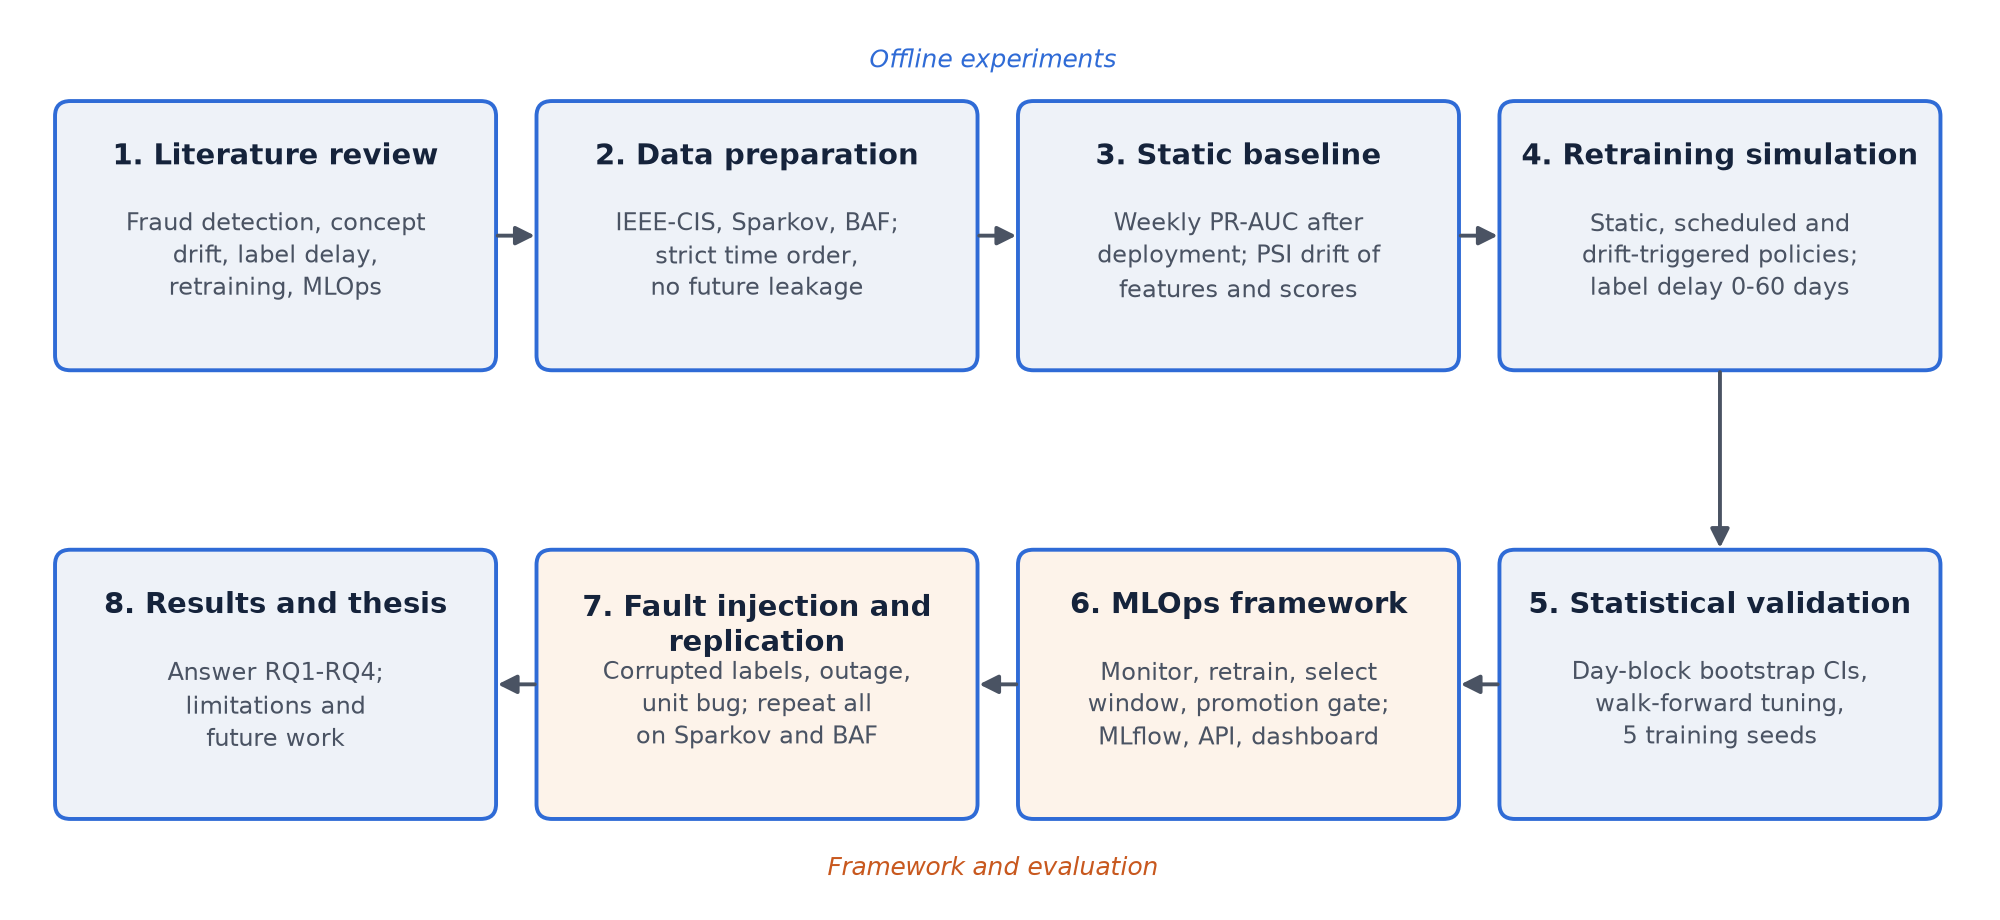
\includegraphics[width=\textwidth]{figures/methodology_3ds.png}
  \caption{Methodology overview: the experiments on three datasets, the framework and its evaluation}
  \label{fig:method3}
\end{figure}

\subsection{Research Design}\label{sec:design}

This study is an empirical, simulation-based investigation followed by the design and evaluation of a software framework. Chapter 2 showed that the claims made for drift-triggered retraining rest mostly on artificial drift, single datasets and labels that arrive immediately \cite{shakil2025,wong2025,yelleti2025}. We therefore first measure, on public fraud data with natural drift, how a deployed model behaves and which retraining policy works best under label delay (research questions RQ1 to RQ3), and only then design the framework around the result and test it (RQ4). The study follows the workflow in Figure \ref{fig:method}.

Three principles guide every experiment. First, \textbf{time is respected}: a model is only trained on transactions that happened, and whose labels were available, before the period it is evaluated on \cite{menezes2025}. Second, \textbf{the deployment is simulated, not imagined}: each dataset is replayed as a stream, week by week, and the label delay is applied explicitly, as described by Dal Pozzolo et al. \cite{dalpozzolo2018}. Third, \textbf{differences must survive uncertainty}: every comparison is reported with a confidence interval, the settings of competing strategies are tuned with the same procedure, and the key results are repeated with several training seeds and on a second dataset.

The rest of this section describes the simulated deployment under label delay (Section \ref{sec:deploy}), the retraining strategies (Section \ref{sec:strategies}), the drift and performance measures (Section \ref{sec:measures}), the statistical validation (Section \ref{sec:validation}) and the evaluation of the framework, including fault injection (Section \ref{sec:faults}). Section \ref{sec:spec} specifies the model and the framework, Sections \ref{sec:collection} and \ref{sec:data} describe the data, Section \ref{sec:plan} the project plan, and Section \ref{sec:impl} the implementation.

\subsection{Simulated Deployment under Label Delay}\label{sec:deploy}

The stream is replayed in steps of seven days, from the stream start to the end of the data. At each step, three things happen in order: the strategy checks which labels are available and decides whether to retrain; if it retrains, a new model is trained and immediately replaces the old one; and the current model scores the transactions of the next seven days. The scores of each week are kept, together with the version of the model that produced them. In production the transactions would arrive through a streaming platform such as Kafka or Flink, as in the real-time pipelines of Kaushik et al. \cite{kaushik2025}; replaying recorded data instead makes every experiment exactly repeatable.

Label delay is modelled as a fixed number of days \textit{d} between a transaction and the moment its label can be used. At time \textit{t}, the labelled data available for monitoring and training is

\begin{equation}
  \mathcal{L}(t) = \{\, x_j : t_j \le t - d \,\}
  \label{eq:labelled}
\end{equation}

where \textit{t\textsubscript{j}} is the time of transaction \textit{x\textsubscript{j}}. The first model is trained at the stream start under the same rule, so it never sees labels it could not have had. We evaluate delays of 0, 15, 30 and 60 days. A delay of 0 corresponds to the assumption made by most retraining studies \cite{yelleti2025,wong2025}; 30 to 60 days corresponds to the time a cardholder typically needs to notice a fraudulent charge and file a dispute \cite{dalpozzolo2018}. Investigator feedback on a few alerted transactions, which arrives faster in a real system \cite{dalpozzolo2018}, is not modelled: every label arrives after the same delay. This makes the setting slightly pessimistic for performance-based triggers, a point we return to in the discussion.

\subsection{Retraining Strategies}\label{sec:strategies}

Five strategies are compared, covering the options described in Section 2.1 \cite{pulicharla2019,dalpozzolo2018}. They are summarised in Table \ref{tab:strategies}.

{\footnotesize
\begin{longtable}{>{\raggedright\arraybackslash}p{0.19\textwidth}>{\raggedright\arraybackslash}p{0.28\textwidth}>{\raggedright\arraybackslash}p{0.23\textwidth}>{\raggedright\arraybackslash}p{0.23\textwidth}}
\caption{Retraining strategies compared in the simulation (default settings)}\label{tab:strategies}\\
\toprule
\textbf{Strategy} & \textbf{When it retrains} & \textbf{Training data} & \textbf{Needs labels to decide?} \\
\midrule
\endfirsthead
\toprule
\textbf{Strategy} & \textbf{When it retrains} & \textbf{Training data} & \textbf{Needs labels to decide?} \\
\midrule
\endhead
Static & Never & History before the stream & - \\ \midrule
Periodic expanding & Every 14 days & All labelled data so far & No \\ \midrule
Periodic sliding & Every 14 days & Labelled data of the last 60 days & No \\ \midrule
Drift: score PSI & PSI of the model's scores over the last week, against its validation scores, exceeds 0.1 (at least 14 days apart) & All labelled data so far & No \\ \midrule
Drift: performance & PR-AUC on newly matured labels falls more than 15\% below the reference (Equation \ref{eq:perftrigger}; at least 14 days apart) & All labelled data so far (or the last 60 days in tuned variants) & Yes (delayed) \\ \bottomrule
\end{longtable}
}

The \textbf{static} model is the reference: it is trained once at the stream start and never updated. The two \textbf{periodic} strategies retrain on a fixed schedule and differ only in their training data: the expanding window uses all labelled data so far, while the sliding window keeps only the most recent 60 days and forgets older patterns.

The \textbf{score-PSI} strategy is a typical label-free drift trigger \cite{shakil2025,wong2025}. It compares the distribution of the scores the model produced over the last week with the scores it produced on its own validation data, using the PSI defined in Section \ref{sec:measures}, and retrains when the PSI exceeds 0.1, the usual boundary between a stable and a shifted population. It can react immediately because it needs no labels.

The \textbf{performance} strategy is an error-based trigger in the spirit of DDM and ADWIN \cite{yelleti2025,aldaoud2025}, adapted to delayed labels. At each step it computes the model's PR-AUC on transactions whose labels matured during the last 14 days and that the model was not trained on, provided they contain at least 30 frauds. It retrains when

\begin{equation}
  \mathrm{AP}_{\mathrm{live}}(t) < (1 - \tau)\, \mathrm{AP}_{\mathrm{ref}}
  \label{eq:perftrigger}
\end{equation}

where AP\textsubscript{live}(\textit{t}) is that live PR-AUC, $\tau$ is the tolerance (0.15 by default), and AP\textsubscript{ref} is either the model's validation PR-AUC or its first live measurement. Both drift strategies wait at least 14 days between retrains, so that one drift episode does not trigger a series of retrains.

Each strategy is run at each label delay, with exactly the same data, model settings and random seed, so that the only difference between runs is the retraining decision and the training window. Models trained on identical windows are cached and reused across strategies, which makes the large number of runs feasible and guarantees that identical decisions give identical models.

\subsection{Drift and Performance Measures}\label{sec:measures}

\textbf{Population Stability Index.} Drift in a feature or in the model's scores is measured with the PSI, which compares a current distribution with a reference distribution \cite{wong2025}:

\begin{equation}
  \mathrm{PSI} = \sum_{i=1}^{B} (c_i - r_i)\,\ln\frac{c_i}{r_i}
  \label{eq:psi}
\end{equation}

where the reference values are divided into \textit{B} = 10 bins at their deciles, \textit{r\textsubscript{i}} and \textit{c\textsubscript{i}} are the shares of reference and current values in bin \textit{i}, missing values form a bin of their own, and shares are floored at 10\textsuperscript{-6} to avoid division by zero. A PSI below 0.1 is usually read as stable, 0.1 to 0.25 as a moderate shift and above 0.25 as a major shift. For the baseline analysis, the PSI is computed for the ten most important features of the static model (by total gain) and for its scores, in every time bin against the training period.

\textbf{PR-AUC.} Fraud is rare and investigators can only review the highest-scored alerts, so the main measure is the area under the precision-recall curve, computed as average precision \cite{dalpozzolo2018}:

\begin{equation}
  \mathrm{AP} = \sum_{n} (R_n - R_{n-1})\,P_n
  \label{eq:ap}
\end{equation}

where \textit{P\textsubscript{n}} and \textit{R\textsubscript{n}} are the precision and recall at the \textit{n}-th threshold of the ranked scores. Unlike accuracy, PR-AUC is not inflated by the large number of legitimate transactions, and unlike ROC-AUC it focuses on how clean the top of the alert list is \cite{abdelnaby2023}. A model with no skill has a PR-AUC equal to the fraud rate.

\textbf{Mean weekly PR-AUC.} In the stream, different weeks are scored by different model versions, whose scores are not calibrated to each other. Computing a single PR-AUC over all weeks would mix these scales and penalise strategies that retrain often, even when every one of their models ranks transactions well. We therefore compute PR-AUC separately for each week \textit{w} of the stream and report the mean over the \textit{W} weeks:

\begin{equation}
  \overline{\mathrm{AP}} = \frac{1}{W} \sum_{w=1}^{W} \mathrm{AP}_w
  \label{eq:weekly}
\end{equation}

Weeks without any fraud are skipped. The lowest weekly PR-AUC, the number of retrains and the F1-score at each model's own threshold are reported as secondary measures.

\subsection{Statistical Validation}\label{sec:validation}

\textbf{Paired day-block bootstrap.} Weekly PR-AUC is noisy, especially when a week contains only a few hundred frauds, and consecutive transactions are correlated. Confidence intervals are therefore computed with a bootstrap that resamples whole days rather than single transactions. Within every week, the days of that week are drawn with replacement, and the mean weekly PR-AUC is recomputed. The same resampled days are used for every strategy, so differences between strategies are paired and much of the shared noise cancels out. We use 500 resamples and report 95\% percentile intervals. A difference is considered reliable when its interval excludes zero.

\textbf{Walk-forward tuning.} A fair comparison requires that every strategy has good settings, chosen without looking at the data it is evaluated on. All 190 configurations in Table \ref{tab:grid} are run over a tuning stream that starts at 35\% of the rows, earlier than the evaluated stream. The evaluated stream is divided into folds of four weeks. At the start of each fold, each family (static, schedule, drift performance) selects the configuration with the highest score

\begin{equation}
  J(c) = \overline{\mathrm{AP}}(c) - \kappa \cdot \frac{N_{\mathrm{retrain}}(c)}{\text{number of 4-week periods}}
  \label{eq:objective}
\end{equation}

computed only on weeks whose labels have matured by the start of the fold, that is, on information that would really have been available. $\kappa$ = 0.002 is a small cost per retrain that breaks ties in favour of simpler configurations. The selected configuration's results on the fold are then recorded, and the next fold repeats the selection. The result is an honest estimate of how each family would perform if an operator tuned it with the information available at the time.

{\footnotesize
\begin{longtable}{>{\raggedright\arraybackslash}p{0.23\textwidth}>{\raggedright\arraybackslash}p{0.47\textwidth}>{\raggedright\arraybackslash}p{0.24\textwidth}}
\caption{Settings searched by walk-forward tuning (190 configurations)}\label{tab:grid}\\
\toprule
\textbf{Family} & \textbf{Settings searched} & \textbf{Configurations} \\
\midrule
\endfirsthead
\toprule
\textbf{Family} & \textbf{Settings searched} & \textbf{Configurations} \\
\midrule
\endhead
Static & - & 1 \\ \midrule
Schedule & Expanding window, period 7, 14 or 28 days; sliding window, period 7, 14 or 28 days and window 30 or 60 days & 9 \\ \midrule
Drift: performance & Tolerance 0.05, 0.1, 0.15, 0.2 or 0.3; monitoring window 7, 14 or 28 days; minimum gap 7, 14 or 28 days; reference = validation PR-AUC or first live measurement; training data = all or last 60 days & 180 \\ \bottomrule
\end{longtable}
}

\textbf{Training seeds.} The bootstrap only covers the randomness of the evaluation sample. LightGBM also has randomness in training, through row and feature subsampling. The key configurations are therefore re-run with five random seeds (42, 1, 2, 3 and 4) at label delays of 0 and 30 days, and for each comparison we report the mean and spread of the difference and the number of seeds in which its sign holds.

\textbf{Replication.} Finally, the whole sequence, from the static baseline through the delay sweep, walk-forward tuning, seeds and the framework replay, is repeated unchanged on Sparkov and BAF, with the same scripts and settings. A finding that holds on IEEE-CIS but not on the other datasets is reported as dataset-specific.

\subsection{Framework Evaluation and Fault Injection}\label{sec:faults}

The framework is evaluated by running it over the evaluated stream of each dataset as if it were live, with a label delay of 30 days. The replay uses the same data store, MLflow registry and model code as a deployment would. Its mean weekly PR-AUC is compared with the offline simulation of the same policy, which checks that the framework reproduces the experimental results, and with the static model. To evaluate window selection, four versions of the framework are replayed on each dataset on the same machine: a static model, a 60-day window, all history, and automatic selection. The four replays share one cache of trained models, so a model with the same training data is trained only once and the versions differ only in their decisions.

A retraining pipeline that runs automatically will eventually train on bad data. To test whether the framework's safeguards stop such models, we inject the faults in Table \ref{tab:faults} into selected retraining jobs of the replay (by default the second and fourth scheduled retrains). The faults imitate common pipeline failures: a misaligned join, an outage of the chargeback feed, and a unit change between training and serving. In the first three, only the data read by the training job is corrupted, while the production feature path and the label store stay correct. The fourth corrupts the label store itself, which the gate also reads, and represents a failure the gate cannot see by design; it tests whether the safety net limits the damage.

{\footnotesize
\begin{longtable}{>{\raggedright\arraybackslash}p{0.23\textwidth}>{\raggedright\arraybackslash}p{0.38\textwidth}>{\raggedright\arraybackslash}p{0.33\textwidth}}
\caption{Faults injected into retraining jobs to test the safeguards}\label{tab:faults}\\
\toprule
\textbf{Fault} & \textbf{What goes wrong} & \textbf{Real-world cause} \\
\midrule
\endfirsthead
\toprule
\textbf{Fault} & \textbf{What goes wrong} & \textbf{Real-world cause} \\
\midrule
\endhead
Label shuffle & Labels are permuted within the training window, so they no longer match their transactions & A misaligned join in the training job \\ \midrule
Label loss & 80\% of frauds in the training window are recorded as legitimate & An outage of the chargeback feed \\ \midrule
Feature unit bug & The five most important numeric features of the live model are multiplied by 100 in training only & A unit change (e.g. cents and dollars) between training and serving \\ \midrule
Upstream label shuffle & The label store itself is corrupted, so the promotion gate also reads wrong labels & Corruption at the source; a known blind spot \\ \bottomrule
\end{longtable}
}

Each fault scenario is replayed twice, once with the promotion gate and once without it, and compared with a clean replay. A safeguard is considered effective if the run with the fault and the safeguard stays close to the clean run, while the run without the safeguard loses performance. Each scenario uses its own MLflow store, so the main registry is never affected.

\section{Design (Model) Specification}\label{sec:spec}

This section specifies the fraud detection model used throughout the study and the components of the drift-aware continuous learning framework.

\subsection{Fraud Detection Model}\label{sec:model}

All experiments use LightGBM, a gradient boosted decision tree library, with the settings in Table \ref{tab:hyper}. Gradient boosted trees are strong and widely used models for tabular fraud data \cite{uddin2026,amekoe2024}, they handle missing values and categorical features natively, and they train fast enough to be retrained hundreds of times. Amekoe et al. also found that batch-trained boosted trees remain competitive with incremental learners when labels arrive late \cite{amekoe2024}, which is exactly the setting of this study. The goal is not to find the best possible classifier, as many static studies do \cite{mienye2023,abdelnaby2023,sohony2018}, but to keep one strong and realistic model fixed so that differences between retraining strategies can be attributed to the strategies alone. No resampling such as SMOTE is used, because it can distort the evaluation \cite{dang2021}; class imbalance is handled by weighting the fraud class instead, a cost-sensitive approach that Somasundaram and Reddy also used to handle imbalance in a drifting fraud stream \cite{somasundaram2019}.

Figure \ref{fig:modelarch} shows the architecture of the model. Each transaction is described by its features, 431 on IEEE-CIS, 16 on Sparkov and 29 on BAF. LightGBM builds an ensemble of decision trees one after another, each with up to 256 leaves, and every new tree is fitted to the errors that the trees before it still make. Training stops when the validation AUC has not improved for 100 rounds, at most after 2,000 trees. For a new transaction, the outputs of all trees are summed into a score \textit{F}(\textit{x}), which a sigmoid function turns into a fraud probability between 0 and 1; the transaction is flagged as fraud when this probability reaches the decision threshold described below.

\begin{figure}[htbp]
  \centering
  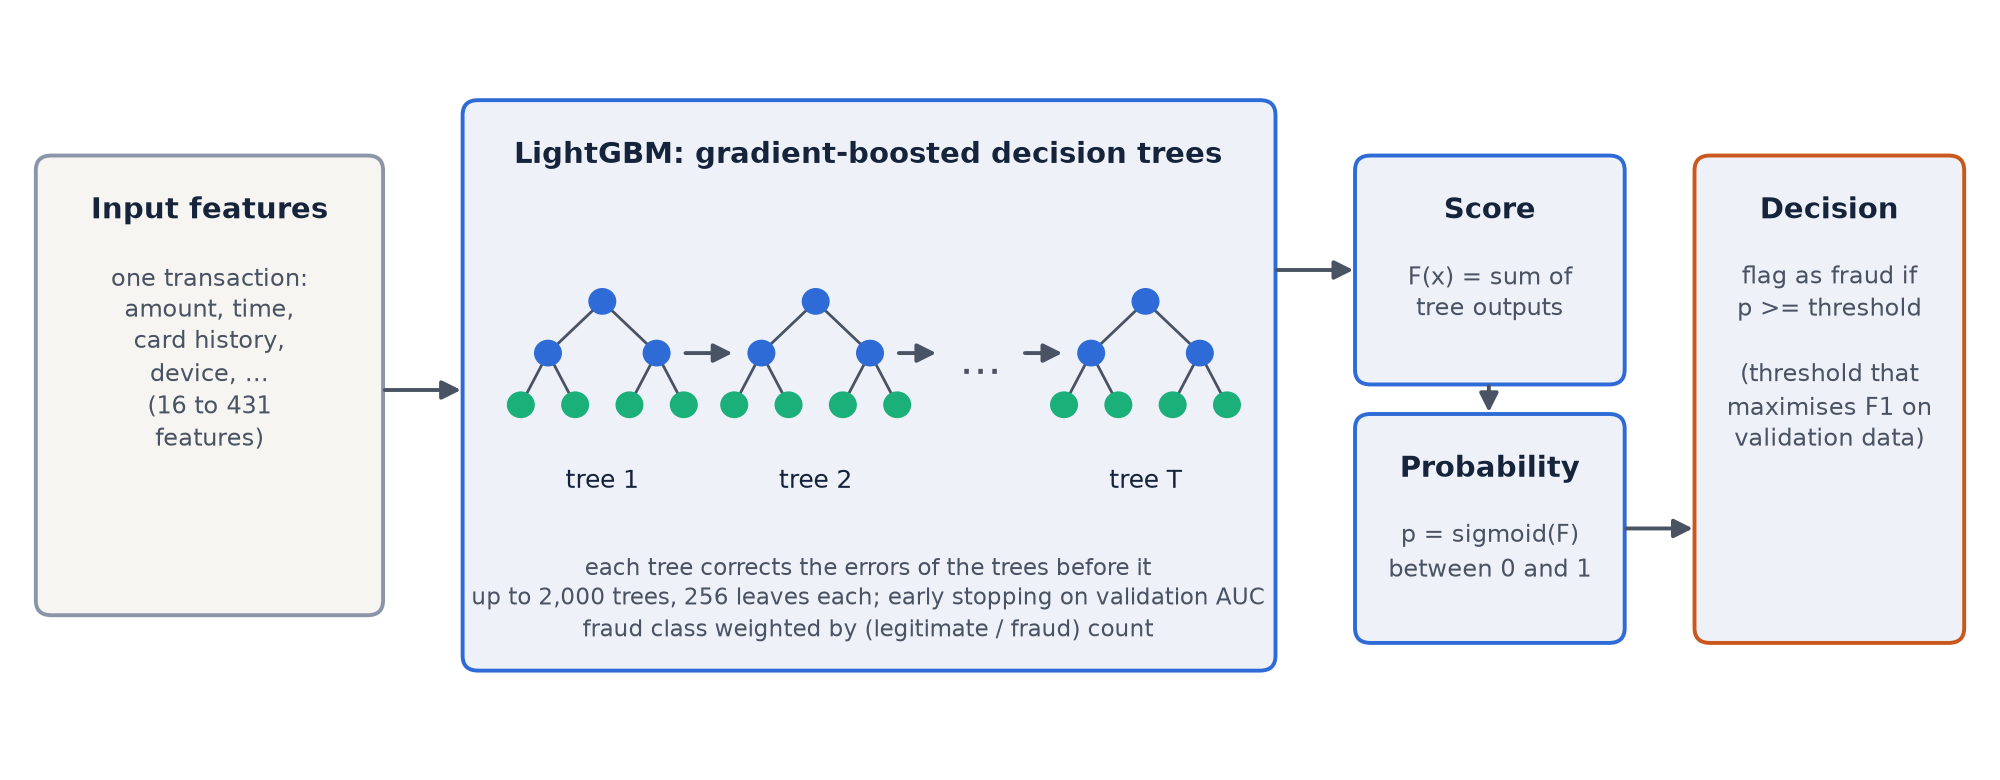
\includegraphics[width=\textwidth]{figures/model_architecture.png}
  \caption{Architecture of the fraud detection model: a transaction's features pass through a sequence of boosted decision trees, whose summed output becomes a fraud probability and, with the validation threshold, a decision}
  \label{fig:modelarch}
\end{figure}

{\footnotesize
\begin{longtable}{>{\raggedright\arraybackslash}p{0.32\textwidth}>{\raggedright\arraybackslash}p{0.19\textwidth}>{\raggedright\arraybackslash}p{0.43\textwidth}}
\caption{LightGBM settings used for every model in the study}\label{tab:hyper}\\
\toprule
\textbf{Setting} & \textbf{Value} & \textbf{Purpose} \\
\midrule
\endfirsthead
\toprule
\textbf{Setting} & \textbf{Value} & \textbf{Purpose} \\
\midrule
\endhead
Objective & binary & Fraud probability for each transaction \\ \midrule
Learning rate & 0.05 & Step size of each boosting round \\ \midrule
Number of leaves & 256 & Capacity of each tree \\ \midrule
Minimum samples per leaf & 100 & Prevents leaves fitted to a few transactions \\ \midrule
Row subsampling & 0.8, every round & Randomness and regularisation \\ \midrule
Feature subsampling & 0.5 per tree & Randomness and regularisation \\ \midrule
L2 regularisation & 1.0 & Shrinks leaf values \\ \midrule
Class weight of fraud & legitimate / fraud count in the training data & Compensates for class imbalance \\ \midrule
Boosting rounds & up to 2,000, early stopping after 100 without improvement & Stops on the validation part of the training window \\ \midrule
Validation part & most recent 15\% of the training window & Early stopping, threshold choice and reference PR-AUC \\ \bottomrule
\end{longtable}
}

Every training run uses a time-ordered validation split: the most recent 15\% of the training window is held out for early stopping, for choosing the decision threshold, and for recording the model's reference PR-AUC. The decision threshold is the one that maximises the F1-score on this validation part. It is used for the F1-score, precision and recall reported alongside PR-AUC and for the fraud flags returned by the scoring service; PR-AUC itself does not depend on a threshold. Alessi and Fugini manage the threshold dynamically during operation to balance precision and recall \cite{alessi2026}; in this design each model keeps the threshold chosen at training time, and a new threshold arrives with every retrained model.

For the static baseline in RQ1, the first 50\% of each dataset is used for training, the next 10\% for validation, and the remaining 40\% is divided into ten consecutive time bins, so that performance can be followed over the months after deployment.

\subsection{Framework Architecture}\label{sec:arch}

The framework turns the experimental findings into a working MLOps system. Its components are shown in Figure \ref{fig:architecture} and its settings in Table \ref{tab:framework}. It runs the loop of Figure \ref{fig:loop} every seven days: monitor, decide, retrain, check, and serve. Like the closed-loop MLOps framework of Reda et al. for phishing detection \cite{reda2025}, it connects monitoring, retraining and deployment in one automated loop; unlike it, its decisions are designed for weeks of label delay rather than near-immediate feedback, so retraining follows a schedule instead of being driven by drift events.

\begin{figure}[htbp]
  \centering
  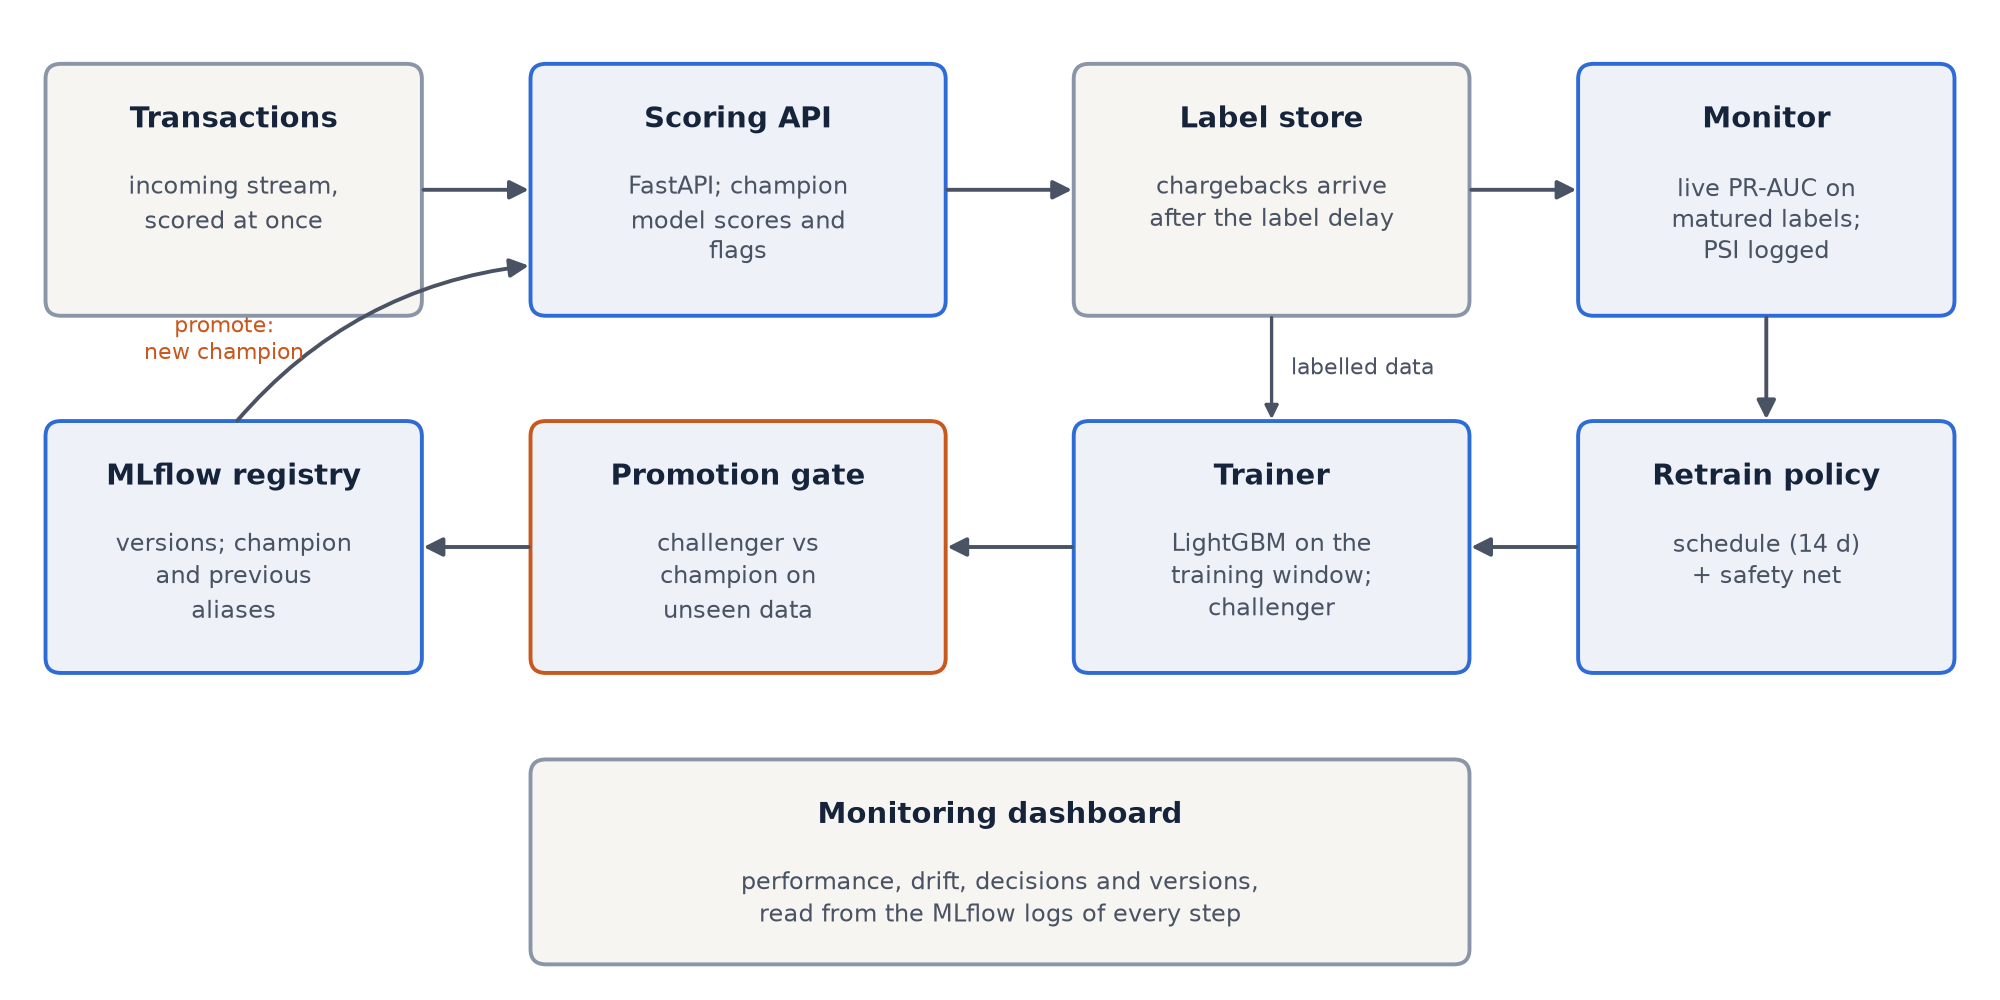
\includegraphics[width=\textwidth]{figures/architecture.png}
  \caption{Components of the proposed framework and the flow of data between them}
  \label{fig:architecture}
\end{figure}

\subsection{Monitoring on Delayed Labels}\label{sec:monitor}

The monitor measures the live model's PR-AUC on the labels that matured during the last 14 days, restricted to transactions the model was not trained on. It also computes the PSI of the model's scores and of its ten most important numeric features against a sample of 50,000 rows of its training window, and logs both to MLflow. In line with the experimental results, the PSI is logged for diagnosis only and never triggers retraining on its own. Two forms of monitoring are deliberately left outside the current design: tracking drift separately for each source of data, as DriftGuard-TriAudit does for the numbers, text and layout of financial statements \cite{hassan2026}, and tracking the stability of model explanations, which John showed can become unstable and unfair as populations drift \cite{john2025}. Both are natural extensions once the framework is used with several data sources or with explanations shown to investigators.

\subsection{Retraining Policy and Safety Net}\label{sec:safety}

The primary policy is a fixed schedule: a new model is trained every 14 days on the last 60 days of labelled data. The schedule is complemented by a \textit{safety net} that retrains early, at most once every seven days, when performance collapses between scheduled retrains:

\begin{equation}
  \mathrm{AP}_{\mathrm{live}} < (1 - \tau)\,\max\big(\mathrm{AP}_{\mathrm{val}},\ \mathrm{median}_{4}(\mathrm{AP}_{\mathrm{live}})\big)\quad\text{or}\quad \mathrm{AP}_{\mathrm{live}} < \lambda\,\pi
  \label{eq:safety}
\end{equation}

with $\tau$ = 0.30, $\lambda$ = 3 and $\pi$ the fraud rate among the matured labels. The first condition compares live PR-AUC with the better of the model's own validation PR-AUC and the median of the last four live measurements. Using recent live history as well as the validation score matters: a model trained on corrupted data can report a poor validation score, which would otherwise lower the bar it is measured against. The second condition is a no-skill check, since a model without skill has a PR-AUC close to the fraud rate.

\subsection{Training and Automatic Window Selection}\label{sec:window}

The trainer fits a LightGBM model with the settings of Table \ref{tab:hyper} on the policy's training window, which ends one label delay before the present. The window length can be set to zero for an expanding window. Each new model is registered in MLflow as a \textit{challenger}, together with its training window, validation PR-AUC and threshold.

\textbf{Automatic window selection.} The experiments showed that the best training window depends on the dataset: the last 60 days on IEEE-CIS, but all labelled history on Sparkov and BAF. A fixed window chosen on one dataset can be wrong for another. The framework can therefore select the window itself. At every retrain it trains one challenger \textit{m\textsubscript{w}} per candidate window \textit{w}, here the last 60 days and all labelled history, and scores all of them on the same evaluation rows \textit{E}: the most recent labelled transactions that none of the candidates was trained on and the champion was not trained on either. It keeps

\begin{equation}
  w^{*} = \arg\max_{w \in \mathcal{W}} \mathrm{AP}_{E}(m_w), \qquad \mathcal{W} = \{\text{60 days},\ \text{all history}\}
  \label{eq:select}
\end{equation}

and only this challenger goes on to the promotion gate; the others are registered as not selected. The choice uses only data that would be available at the time, so it needs no knowledge of which window suits the dataset. Because the candidates are trained on identical data except for their start date, the extra cost is one additional training run per retrain.

\subsection{Promotion Gate}\label{sec:gate}

A challenger replaces the live model (the \textit{champion}) only if it passes the promotion gate, following the champion-challenger pattern of MLOps practice \cite{pulicharla2019,kodakandla2024}. The gate compares both models on the challenger's validation data, restricted to transactions that the champion was not trained on, so that neither model is judged on data it has seen. The challenger is promoted if

\begin{equation}
  \mathrm{AP}(\text{challenger}) \ge \mathrm{AP}(\text{champion}) - \delta
  \label{eq:gate}
\end{equation}

with $\delta$ = 0.01. Both models are re-scored through the production feature path rather than with scores stored at training time. This detail is essential: a model trained on wrongly scaled features looks good on its own, equally wrong, validation data, but fails on the inputs it will actually receive in production. If the comparison data contains fewer than 30 frauds, the comparison is not reliable and the challenger is promoted by default.

\subsection{Framework Configuration}\label{sec:config}

{\footnotesize
\begin{longtable}{>{\raggedright\arraybackslash}p{0.32\textwidth}>{\raggedright\arraybackslash}p{0.15\textwidth}>{\raggedright\arraybackslash}p{0.47\textwidth}}
\caption{Settings of the framework (configs/default.toml)}\label{tab:framework}\\
\toprule
\textbf{Setting} & \textbf{Value} & \textbf{Meaning} \\
\midrule
\endfirsthead
\toprule
\textbf{Setting} & \textbf{Value} & \textbf{Meaning} \\
\midrule
\endhead
Loop interval & 7 days & How often the framework monitors, decides and serves \\ \midrule
Label delay d & 30 days & Labels usable this long after the transaction \\ \midrule
Retraining schedule & 14 days & Primary policy \\ \midrule
Training window & 60 days & Sliding window of labelled data (0 = expanding) \\ \midrule
Candidate windows & 60 days, all & With automatic selection: one challenger per window, the best one is gated \\ \midrule
Monitoring window & 14 days & Matured labels used for live PR-AUC \\ \midrule
Minimum frauds & 30 & Fewer frauds: live PR-AUC is not computed \\ \midrule
Safety-net tolerance $\tau$ & 0.30 & Relative drop that triggers an early retrain \\ \midrule
History for the reference & 4 & Recent live measurements in the median \\ \midrule
No-skill factor $\lambda$ & 3 & Live PR-AUC below 3 x fraud rate triggers \\ \midrule
Minimum gap between retrains & 7 days & Prevents repeated early retrains \\ \midrule
Gate tolerance $\delta$ & 0.01 & Largest PR-AUC loss a challenger may show \\ \midrule
Gate minimum frauds & 30 & Fewer frauds: the challenger is promoted by default \\ \midrule
Drift features tracked & 10 & Most important numeric features (PSI logged) \\ \bottomrule
\end{longtable}
}

\section{Data Collection}\label{sec:collection}

The study uses three public fraud datasets, summarised in Table \ref{tab:sources}. Public data with reliable timestamps is essential for the research questions, because drift and label delay can only be studied when transactions can be replayed in the order in which they happened. Commonly used fraud datasets that cover only a few days \cite{dang2021,mienye2023} were therefore not suitable.

{\footnotesize
\begin{longtable}{>{\raggedright\arraybackslash}p{0.15\textwidth}>{\raggedright\arraybackslash}p{0.32\textwidth}>{\raggedright\arraybackslash}p{0.23\textwidth}>{\raggedright\arraybackslash}p{0.24\textwidth}}
\caption{Sources of the datasets}\label{tab:sources}\\
\toprule
\textbf{Dataset} & \textbf{Source} & \textbf{Files used} & \textbf{Records in the source} \\
\midrule
\endfirsthead
\toprule
\textbf{Dataset} & \textbf{Source} & \textbf{Files used} & \textbf{Records in the source} \\
\midrule
\endhead
IEEE-CIS & Kaggle competition IEEE-CIS Fraud Detection (IEEE Computational Intelligence Society and Vesta Corporation) & train\_transaction.csv, train\_identity.csv & 590,540 transactions \\ \midrule
Sparkov & Kaggle dataset Credit Card Transactions Fraud Detection (generated with the Sparkov simulator) & fraudTrain.csv, fraudTest.csv & 1,852,394 transactions \\ \midrule
BAF & Kaggle dataset Bank Account Fraud Dataset Suite (NeurIPS 2022) & Base.csv (of six variants) & 1,000,000 applications \\ \bottomrule
\end{longtable}
}

All three datasets were downloaded from Kaggle. IEEE-CIS is distributed as a competition dataset, which requires accepting the competition rules; its test files have no labels and were not used. Sparkov is distributed as two files that split one continuous period, and both were combined. BAF is distributed as a base dataset and five variants with controlled biases; the base dataset was used. The raw data is not redistributed with the code: the repository contains the scripts that prepare it, so that every result can be regenerated from the original sources.

Two practical choices made the data collection reproducible. First, every dataset is converted by a preparation script into the same table layout, so all experiments run unchanged on any of them. Second, the long experiments on the two larger replication datasets were run as Kaggle notebooks, next to the data, with the code taken directly from the public repository.

\section{Dataset Overview}\label{sec:data}

This section describes each dataset, the target variable, the cleaning and feature engineering applied to it, and the resulting preprocessed data.

\subsection{IEEE-CIS Fraud Detection}\label{sec:ieeecis}

IEEE-CIS is the main dataset. It was released by the IEEE Computational Intelligence Society and Vesta Corporation and contains 590,540 real e-commerce transactions over 182 days, of which 3.5\% are fraudulent. It has been used in recent studies of drift and fraud detection \cite{menezes2025,uddin2026}. The transaction and identity tables are joined on the transaction identifier, giving 431 features, most of them anonymised by the provider. Only the time column (seconds from a reference point), the identifier and the label are excluded. Text columns are treated as categorical features, which LightGBM handles natively, and missing values are kept as missing rather than imputed. More than half of the columns are missing for over 50\% of transactions.

\subsection{Sparkov Credit Card Transactions}\label{sec:sparkovds}

Sparkov is the first replication dataset. It contains card transactions for about 1,000 customers produced by the Sparkov transaction simulator between January 2019 and December 2020. After inspection we cut the data at 21 December 2020, because the simulator produces almost no fraud after that date (17 frauds and then none, while the volume doubles), which would make the last weeks meaningless for evaluation. The remaining 1,801,969 transactions cover 720 days with a fraud rate of 0.53\%. Names, street addresses, card numbers and transaction numbers are removed. We derive the transaction hour and weekday, the customer's age, and the distance between customer and merchant, and five per-card behaviour features: the time since the card's previous transaction, its number and total amount of transactions in the previous 24 hours, its number of transactions in the previous 30 days, and the amount relative to the card's running average. Each of these is computed only from the card's \textit{earlier} transactions, so no information from the future leaks into a feature. A lifetime transaction count was deliberately not used: it only grows over time and would drift by construction.

\subsection{Bank Account Fraud (BAF)}\label{sec:bafds}

BAF is the second replication dataset. It is a privacy-preserving synthetic dataset of one million bank account applications over eight months, generated from real data and designed to contain realistic drift between months. We use the Base variant. Values that the providers document as missing (negative values in six columns) are converted to missing values, a constant column is dropped, and the month itself is not used as a feature, so that the model cannot memorise the period. BAF records only the month of each application, so each record is given a random time within its month with a fixed seed. Drift therefore appears between months, while the weeks within a month are exchangeable. This is a limitation of the dataset, and the BAF results are interpreted accordingly.

\subsection{Target Variable and Class Imbalance}\label{sec:target}

The target is a binary label that marks a transaction, or an application in the case of BAF, as fraudulent (1) or legitimate (0). It is called isFraud in IEEE-CIS, is\_fraud in Sparkov and fraud\_bool in BAF, and is renamed isFraud in all three. Fraud is rare in every dataset: there are 27.6 legitimate transactions per fraud in IEEE-CIS, 186.1 in Sparkov and 89.7 in BAF. For this reason accuracy is not used as a measure (a model that never predicts fraud would be 96.5\% to 99.5\% accurate), and PR-AUC is the main measure (Section \ref{sec:measures}). The imbalance is handled by weighting the fraud class in training; no oversampling such as SMOTE is used, because resampling can make results look better than they are \cite{dang2021}.

\subsection{Data Cleaning and Feature Engineering}\label{sec:cleaning}

The preprocessing pipeline is shown in Figure \ref{fig:preproc}. In IEEE-CIS, the transaction and identity tables are joined on the transaction identifier, numeric columns are stored in the smallest suitable type to reduce memory, and the 31 text columns are converted to categorical features. Missing values are kept as missing, because LightGBM handles them natively and because missingness itself can carry information: 214 of the 434 columns are missing for more than half of the transactions.

In Sparkov, names, street addresses, card numbers and transaction numbers are removed, and the data is cut at 21 December 2020, after which the simulator produces almost no fraud; this keeps 1,801,969 of 1,852,394 transactions. Time-of-day, weekday, age and the distance between customer and merchant are derived, and five per-card behaviour features are computed only from each card's earlier transactions, so that no information leaks from the future. In BAF, values documented as missing (negative values in six columns) are converted to missing, a constant column is dropped, and the month is not used as a feature.

\begin{figure}[htbp]
  \centering
  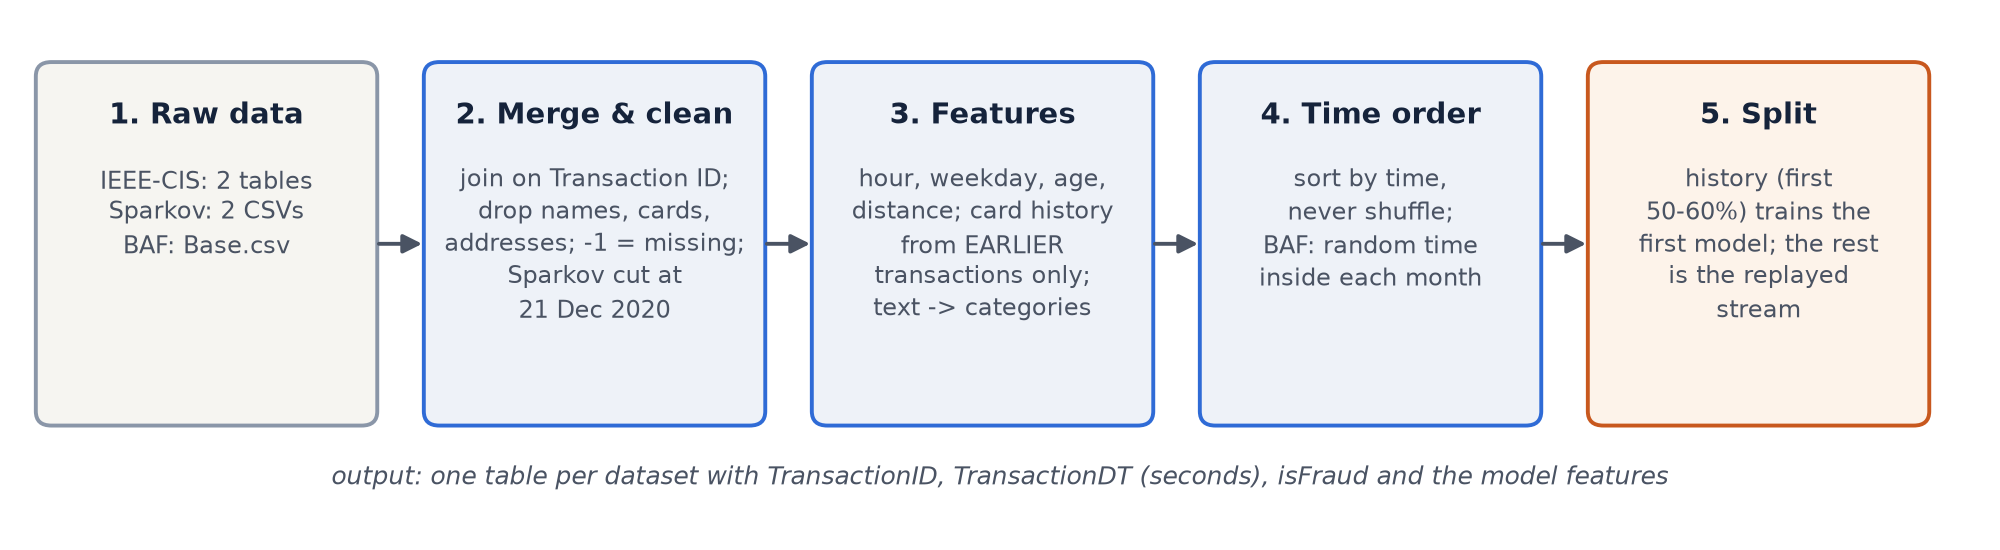
\includegraphics[width=\textwidth]{figures/preprocessing.png}
  \caption{Preprocessing pipeline from the raw files of each dataset to the common time-ordered table}
  \label{fig:preproc}
\end{figure}

\subsection{Time Ordering and History-Stream Split}\label{sec:split}

All three datasets are sorted by time and never shuffled. Each is split at a fixed fraction of its rows into a \textit{history}, used to train the first model, and a \textit{stream}, which is replayed as if it were arriving live (Figure \ref{fig:protocol}). The stream starts at 60\% of the rows for IEEE-CIS (day 101), and at 50\% for Sparkov and BAF, whose longer histories allow a full year or four months of training data before deployment.

\begin{figure}[htbp]
  \centering
  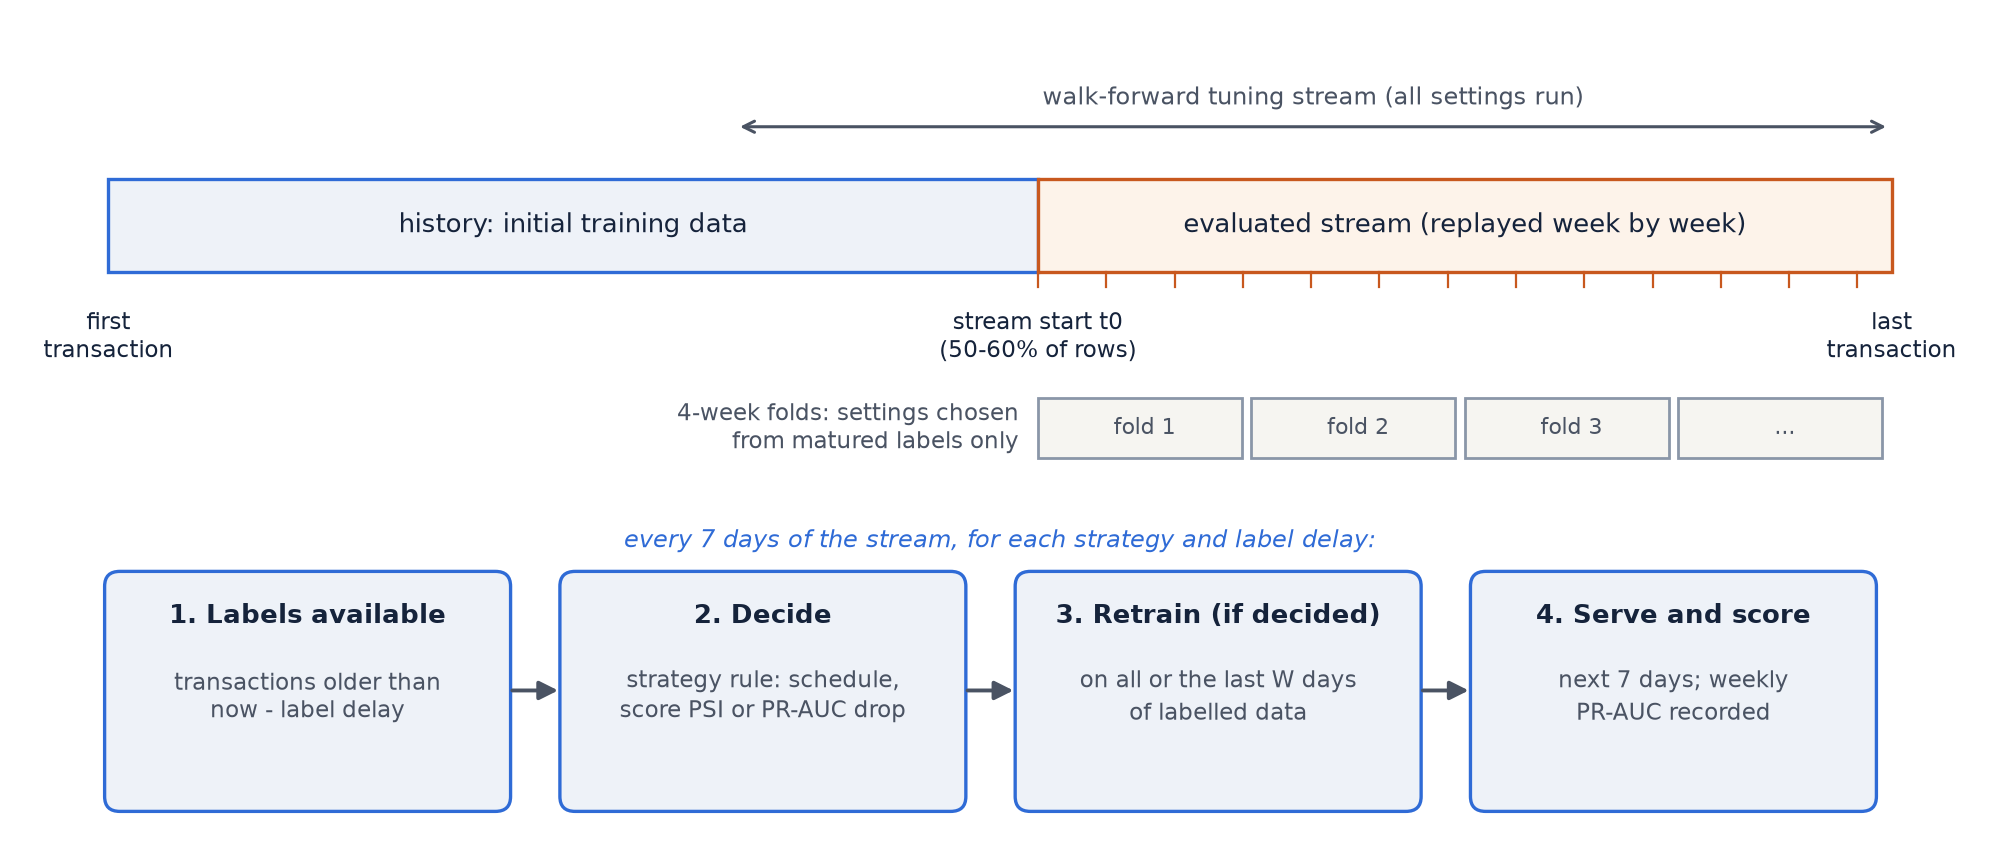
\includegraphics[width=\textwidth]{figures/protocol.png}
  \caption{Evaluation protocol: each dataset is split in time into a history and a stream that is replayed week by week; settings are tuned walk-forward in 4-week folds}
  \label{fig:protocol}
\end{figure}

\subsection{Summary of Preprocessed Data}\label{sec:summarydata}

Table \ref{tab:preprocessed} summarises the data after preprocessing, and Table \ref{tab:datasets} compares the three datasets. Every prepared dataset is a single table with a transaction identifier, a time column in seconds, the isFraud label and the model features, sorted by time.

{\footnotesize
\begin{longtable}{>{\raggedright\arraybackslash}p{0.32\textwidth}>{\raggedright\arraybackslash}p{0.21\textwidth}>{\raggedright\arraybackslash}p{0.21\textwidth}>{\raggedright\arraybackslash}p{0.21\textwidth}}
\caption{Summary of the preprocessed data}\label{tab:preprocessed}\\
\toprule
\textbf{} & \textbf{IEEE-CIS} & \textbf{Sparkov} & \textbf{BAF} \\
\midrule
\endfirsthead
\toprule
\textbf{} & \textbf{IEEE-CIS} & \textbf{Sparkov} & \textbf{BAF} \\
\midrule
\endhead
Records after preprocessing & 590,540 & 1,801,969 & 1,000,000 \\ \midrule
Frauds (rate) & 20,663 (3.50\%) & 9,634 (0.53\%) & 11,029 (1.10\%) \\ \midrule
Legitimate per fraud & 27.6 & 186.1 & 89.7 \\ \midrule
Features (of which categorical) & 431 (31) & 16 (5) & 29 (5) \\ \midrule
History: training the first model & 354,324 (60\%) & 900,984 (50\%) & 500,000 (50\%) \\ \midrule
Stream: replayed week by week & 236,216 (12 weeks) & 900,985 (52 weeks) & 500,000 (19 weeks) \\ \bottomrule
\end{longtable}
}

{\footnotesize
\begin{longtable}{>{\raggedright\arraybackslash}p{0.16\textwidth}>{\raggedright\arraybackslash}p{0.26\textwidth}>{\raggedright\arraybackslash}p{0.26\textwidth}>{\raggedright\arraybackslash}p{0.25\textwidth}}
\caption{Datasets used in this study (after preparation)}\label{tab:datasets}\\
\toprule
\textbf{} & \textbf{IEEE-CIS} & \textbf{Sparkov} & \textbf{BAF (Base)} \\
\midrule
\endfirsthead
\toprule
\textbf{} & \textbf{IEEE-CIS} & \textbf{Sparkov} & \textbf{BAF (Base)} \\
\midrule
\endhead
Domain & Real e-commerce card transactions (Vesta) & Simulated card transactions (Sparkov generator) & Bank account opening applications (privacy-preserving synthetic data) \\ \midrule
Records & 590,540 & 1,801,969 & 1,000,000 \\ \midrule
Time span & 182 days & 720 days (to 21 Dec 2020) & 8 months \\ \midrule
Fraud rate & 3.50\% & 0.53\% & 1.10\% \\ \midrule
Features used & 431 (transaction and identity tables, mostly anonymised) & 16 (amount, time, location, customer and card-history features) & 29 (applicant, request, device and velocity features) \\ \midrule
Time resolution & Seconds from a reference point & Exact timestamp & Month only (time within the month assigned at random) \\ \midrule
Stream starts at & 60\% of rows (day 101) & 50\% of rows (about 1 Jan 2020) & 50\% of rows (month 4) \\ \midrule
Role & Main dataset & Replication & Second replication \\ \bottomrule
\end{longtable}
}

\section{Project Management Plan}\label{sec:plan}

The project was organised in three stages that match the thesis deliverables, as shown in Figure \ref{fig:plan}. The first stage covered the literature review, the research questions and the preparation of IEEE-CIS. The second stage covered the experiments, their statistical validation and the design of the framework. The third stage covered the framework's evaluation, the replication on two further datasets, automatic window selection and the changes requested in supervisor feedback.

\begin{figure}[htbp]
  \centering
  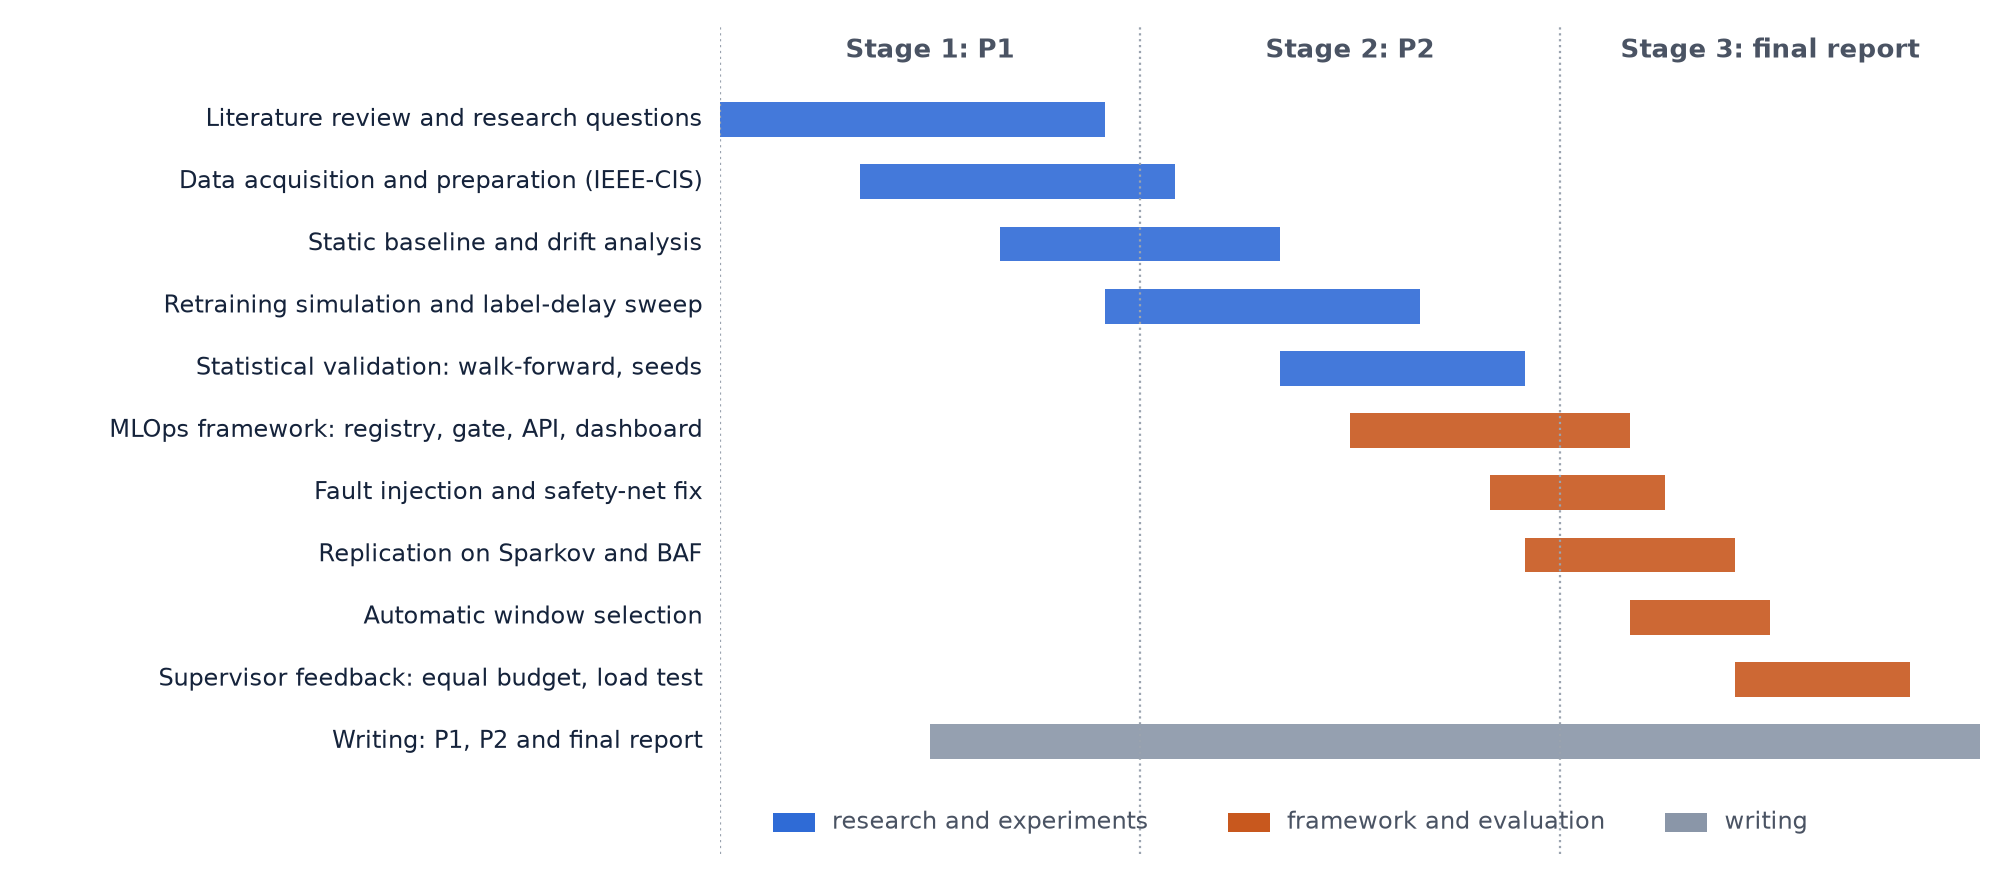
\includegraphics[width=\textwidth]{figures/project_plan.png}
  \caption{Project management plan over the three thesis stages}
  \label{fig:plan}
\end{figure}

Work proceeded in short iterations: each experiment was planned, run, reviewed and, when its result raised a new question, followed by a further experiment. Several design decisions came out of this cycle. The walk-forward tuning was added when fixed tuning periods proved too short to rank the drift triggers; the promotion gate was changed to re-score models on production features after a fault test exposed a weakness; and automatic window selection was added when the replication showed that the best window depends on the dataset. Supervisor feedback was incorporated in the same way, for example the equal-budget comparison in Section \ref{sec:budget}.

All code and configuration were kept under version control in a Git repository hosted on GitHub, with an automated test suite run before each change. Because single experiments ran for several hours and power cuts were frequent, the long experiments save their results after every completed step and resume where they stopped; the longest runs were moved to Kaggle notebooks.

\section{Implementation of Selected Design}\label{sec:impl}

The selected design was implemented as a Python package with a back end that runs the continuous learning loop, a front end for monitoring, and a model registry that connects them. Table \ref{tab:modules} lists the modules.

\subsection{Back End}\label{sec:backend}

{\footnotesize
\begin{longtable}{>{\raggedright\arraybackslash}p{0.21\textwidth}>{\raggedright\arraybackslash}p{0.73\textwidth}}
\caption{Modules of the framework (Python package fraud\_mlops)}\label{tab:modules}\\
\toprule
\textbf{Module} & \textbf{Responsibility} \\
\midrule
\endfirsthead
\toprule
\textbf{Module} & \textbf{Responsibility} \\
\midrule
\endhead
config & Typed configuration loaded from one TOML file per dataset \\ \midrule
data & Loading, caching and time-window access to the transaction table \\ \midrule
training & LightGBM training on a window with a time-ordered validation split \\ \midrule
model & Scoring of raw input, including missing columns and text categories \\ \midrule
monitoring & Live PR-AUC on matured labels; PSI of scores and features \\ \midrule
policy & Retraining policy, safety net, candidate windows and promotion gate \\ \midrule
registry & MLflow runs and model registry with champion and previous aliases \\ \midrule
pipeline & The replay loop: monitor, decide, retrain, gate and serve \\ \midrule
faults & Fault injection for testing the safeguards \\ \midrule
serving & FastAPI scoring service for the champion model \\ \midrule
dashboard & Self-contained HTML monitoring dashboard \\ \midrule
cli & Command line: replay, champion, dashboard and serve \\ \bottomrule
\end{longtable}
}

The study is implemented in Python with LightGBM, pandas, NumPy and scikit-learn for the experiments, MLflow with an SQLite backend for tracking and the model registry, and FastAPI for the scoring service. The framework is organised as a Python package with separate modules for configuration, data access, training, monitoring, the retraining policy, the promotion gate, the registry, fault injection, serving and the dashboard, and is configured with one TOML file per dataset. Twenty-four automated tests on small synthetic data check the components and the full loop.

The back end is driven from the command line. \textit{replay} runs the loop over a dataset as if it were live, \textit{champion} reports the model in service, \textit{dashboard} builds the monitoring dashboard and \textit{serve} starts the scoring service. Every training run is logged to MLflow with its parameters, metrics and training window, and every model is registered as a new version.

\subsection{Front End}\label{sec:frontend}

The front end is a monitoring dashboard, generated as a single HTML page from the MLflow logs of a replay, that can be opened in any browser without a server. It shows the summary figures of the run, the weekly performance of the served model together with what the loop could measure on delayed labels and the safety-net line (Figure \ref{fig:dashtop}), the drift measures, every retraining decision with its reason, and the history of model versions with the champion and the version kept for rollback (Figure \ref{fig:dashlog}).

\begin{figure}[htbp]
  \centering
  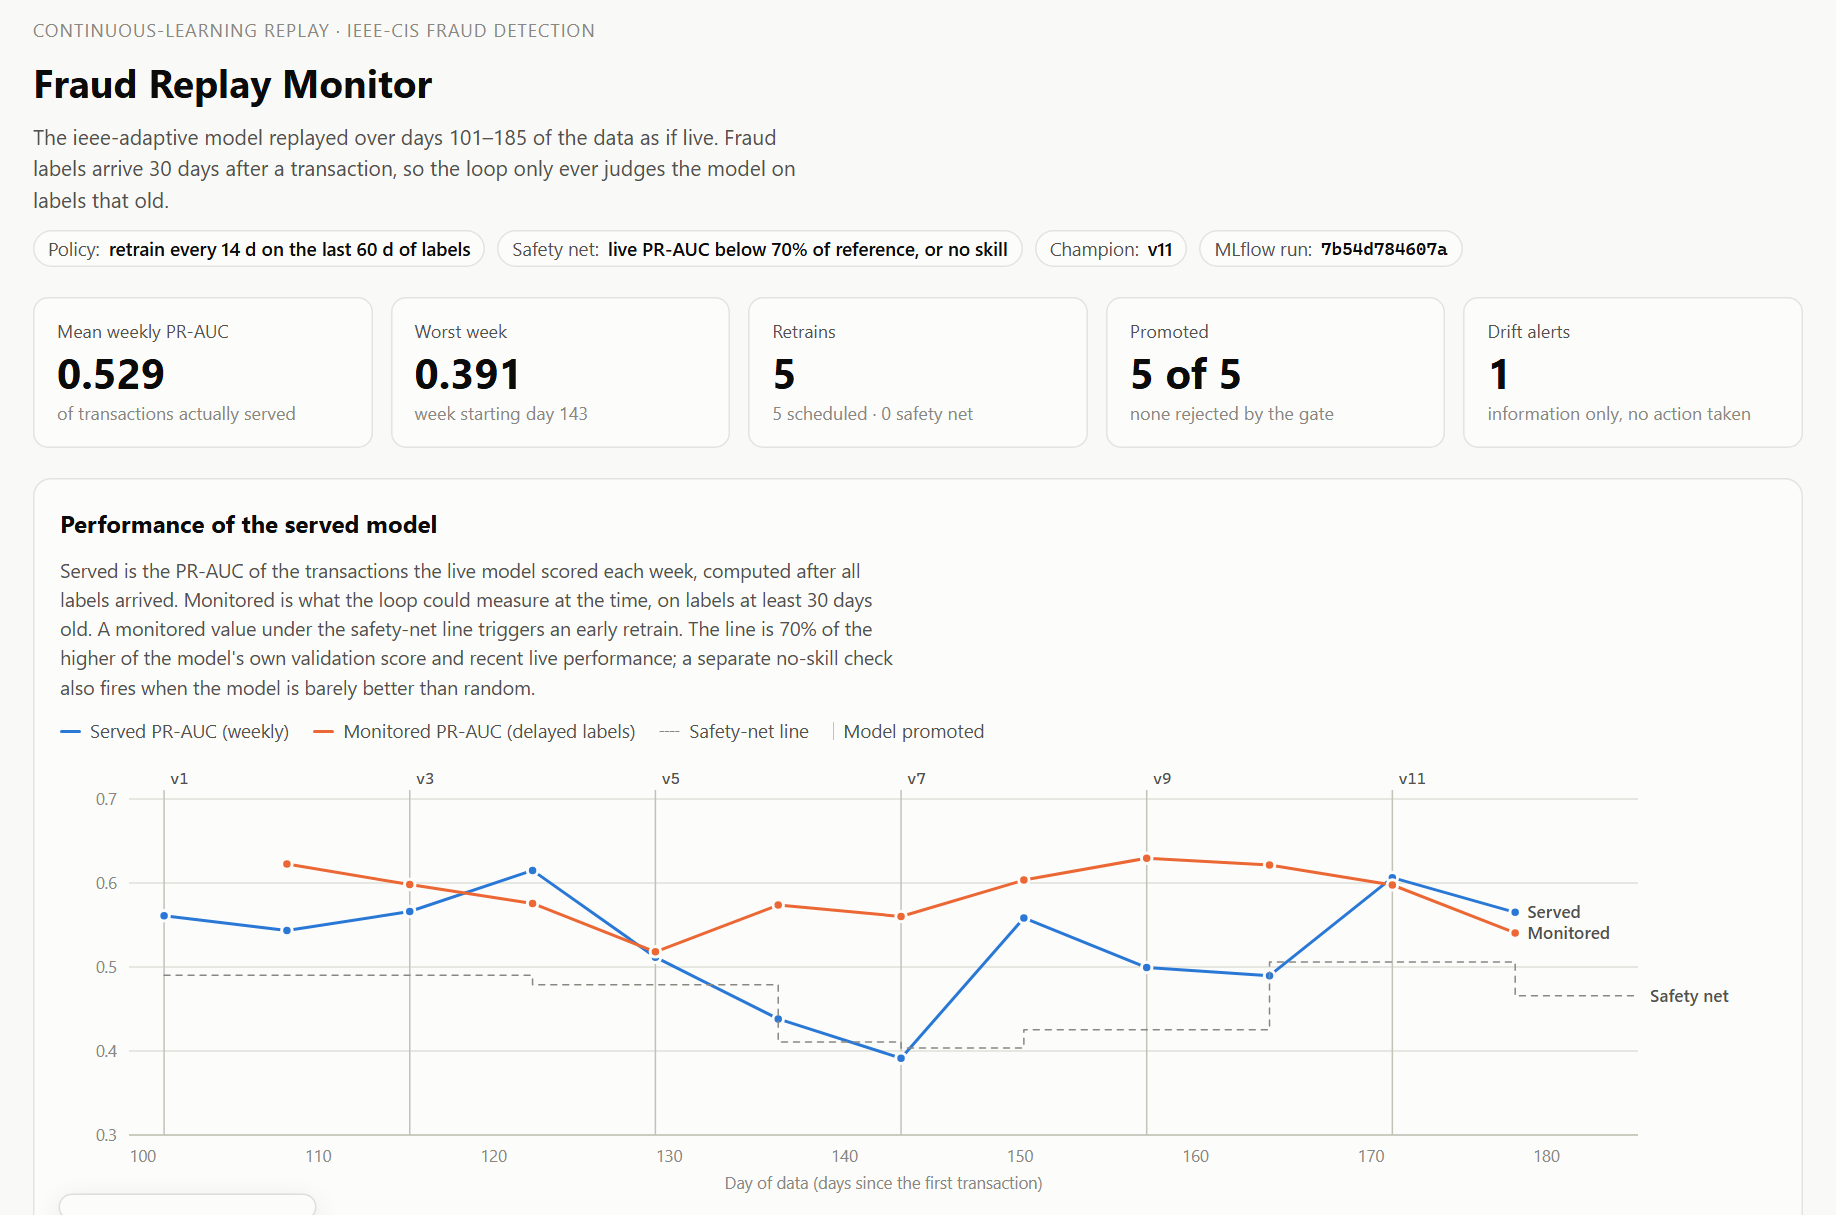
\includegraphics[width=\textwidth]{figures/dashboard_top.png}
  \caption{Front end: the monitoring dashboard after a replay of IEEE-CIS (summary figures and the performance of the served model)}
  \label{fig:dashtop}
\end{figure}

\begin{figure}[htbp]
  \centering
  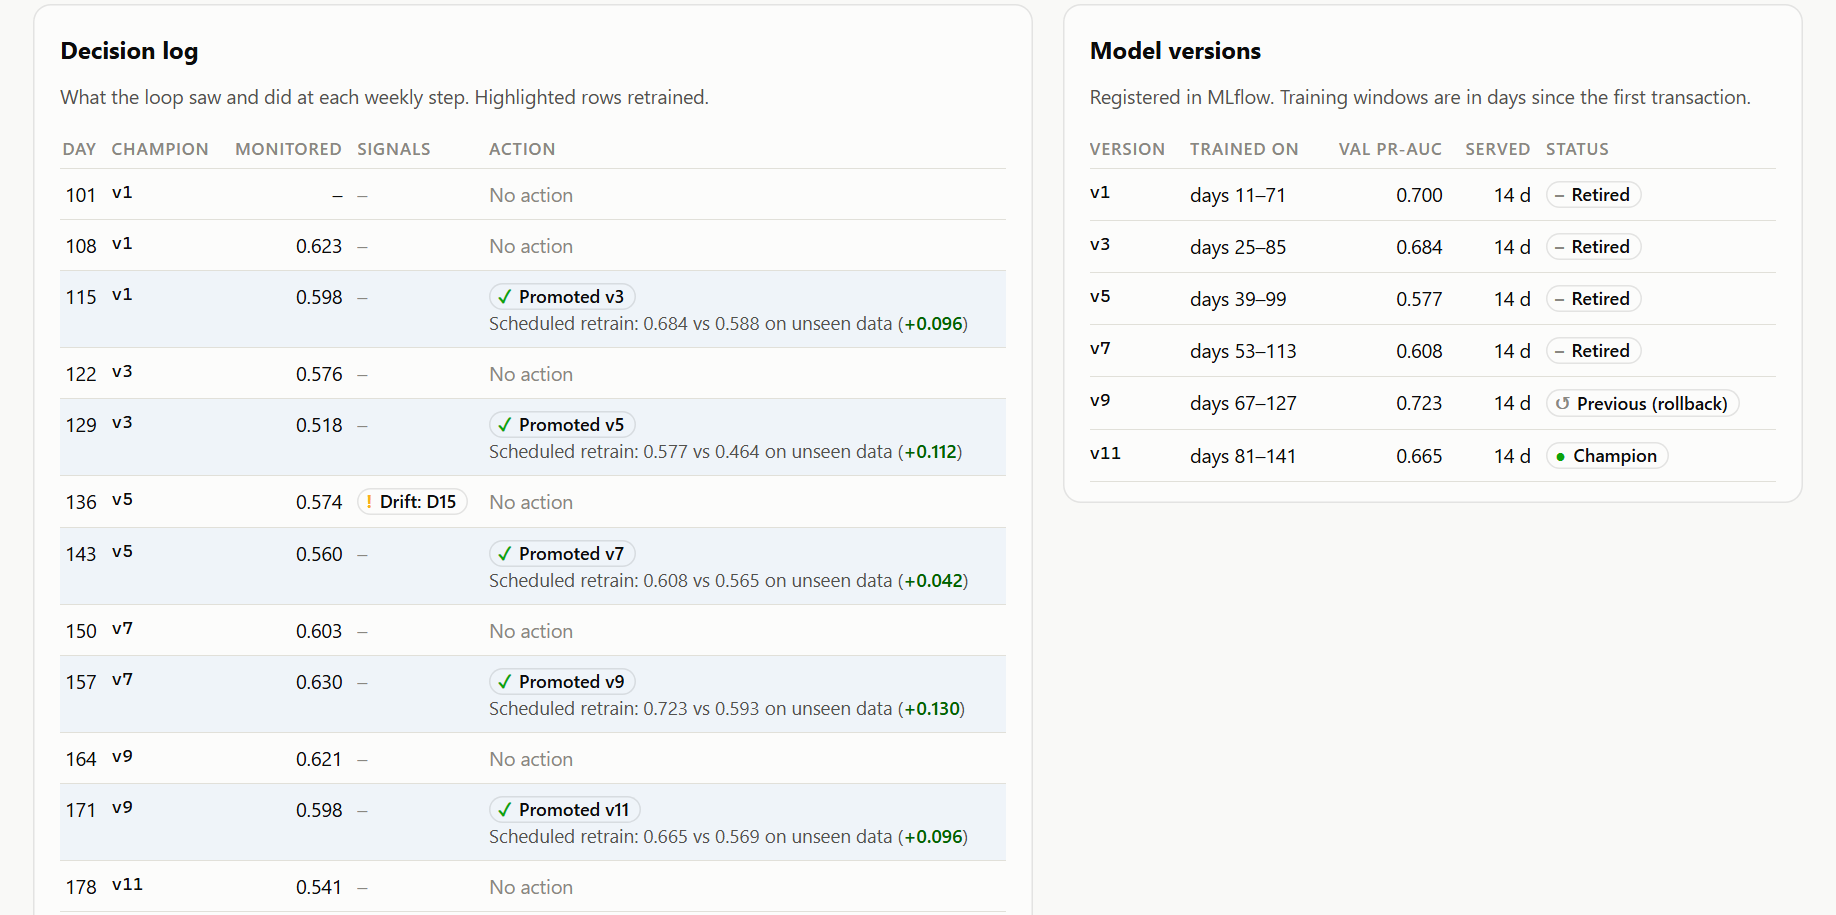
\includegraphics[width=\textwidth]{figures/dashboard_log.png}
  \caption{Front end: decision log and model versions on the monitoring dashboard}
  \label{fig:dashlog}
\end{figure}

\subsection{Frontend-Backend Integration}\label{sec:integration}

MLflow stores every model version with its parameters, metrics and training window. The model in service carries the alias \textit{champion} and its predecessor the alias \textit{previous}, so a rollback is a single alias change. A FastAPI service loads the champion and offers three endpoints: \textit{/health} reports the version being served, \textit{/predict} returns a fraud probability and flag for each submitted transaction, and \textit{/reload} switches to a newly promoted champion without restarting. A monitoring dashboard, generated from the MLflow logs, shows weekly performance, drift, every retraining decision with its reason, and the history of model versions.

The MLflow model registry is the contract between the parts: the back end writes model versions and moves the \textit{champion} alias when the promotion gate accepts a challenger, the scoring service loads whatever carries that alias and reloads it on request, and the dashboard reads the same registry and run logs. No component needs to know how the others work, so the scoring service always serves the model the gate last approved.

\chapter{Result Analysis}

\section{Performance Evaluation}\label{sec:evaluation}

\subsection{Testing Method}\label{sec:testing}

The framework and the retraining strategies are tested by replaying each dataset in strict time order, as described in Section \ref{sec:overview}. A model is trained on the history, deployed at the start of the stream and scores each following week before the labels of that week are known; the labels become usable only after the label delay of 0, 15, 30 or 60 days. Every strategy starts from the same initial model and sees exactly the same data, so differences between strategies come only from their retraining decisions. The framework itself is tested by a full replay with its registry, monitor and promotion gate (Section \ref{sec:replay5}) and by injecting faults into its retraining jobs (Section \ref{sec:faults5}).

\subsection{Evaluation Metrics}\label{sec:metrics}

The main metric is the mean weekly PR-AUC (Equation \ref{eq:weekly}), computed per week so that scores of different model versions are never pooled. ROC-AUC, precision, recall and F1 at each model's validation threshold, the lowest weekly PR-AUC and the number of retrains are reported as secondary measures. Drift is measured with the PSI (Equation \ref{eq:psi}). Differences between strategies are reported with 95\% paired day-block bootstrap intervals, and a difference is called reliable when its interval excludes zero. Because the datasets differ in difficulty, a model without skill would score 0.035 on IEEE-CIS, 0.005 on Sparkov and 0.011 on BAF, so PR-AUC values are compared within a dataset only.

\subsection{Model Performance and Drift after Deployment}\label{sec:rq1}

Table \ref{tab:decay} and Figure \ref{fig:decay} show how the static model performed over the test period of each dataset, which follows the training and validation periods in time.

{\footnotesize
\begin{longtable}{>{\raggedright\arraybackslash}p{0.32\textwidth}>{\raggedright\arraybackslash}p{0.21\textwidth}>{\raggedright\arraybackslash}p{0.21\textwidth}>{\raggedright\arraybackslash}p{0.21\textwidth}}
\caption{Performance of the static model and drift of its inputs after deployment}\label{tab:decay}\\
\toprule
\textbf{} & \textbf{IEEE-CIS} & \textbf{Sparkov} & \textbf{BAF} \\
\midrule
\endfirsthead
\toprule
\textbf{} & \textbf{IEEE-CIS} & \textbf{Sparkov} & \textbf{BAF} \\
\midrule
\endhead
PR-AUC over the whole test period & 0.510 & 0.936 & 0.164 \\ \midrule
ROC-AUC over the whole test period & 0.888 & 0.997 & 0.871 \\ \midrule
PR-AUC, first time bin & 0.581 & 0.954 & 0.164 \\ \midrule
PR-AUC, lowest time bin & 0.388 (bin 6) & 0.893 (bin 10) & 0.149 (bin 6) \\ \midrule
PR-AUC, last time bin & 0.534 & 0.893 & 0.169 \\ \midrule
Largest feature PSI (feature) & 0.17 (D10) & 0.53 (card\_txns\_24h) & 4.60 (velocity\_4w) \\ \midrule
Score-PSI trigger (threshold 0.1) & never fired; maximum score PSI 0.017 & fired once (1 of 4 label delays) & never fired \\ \bottomrule
\end{longtable}
}

\begin{figure}[htbp]
  \centering
  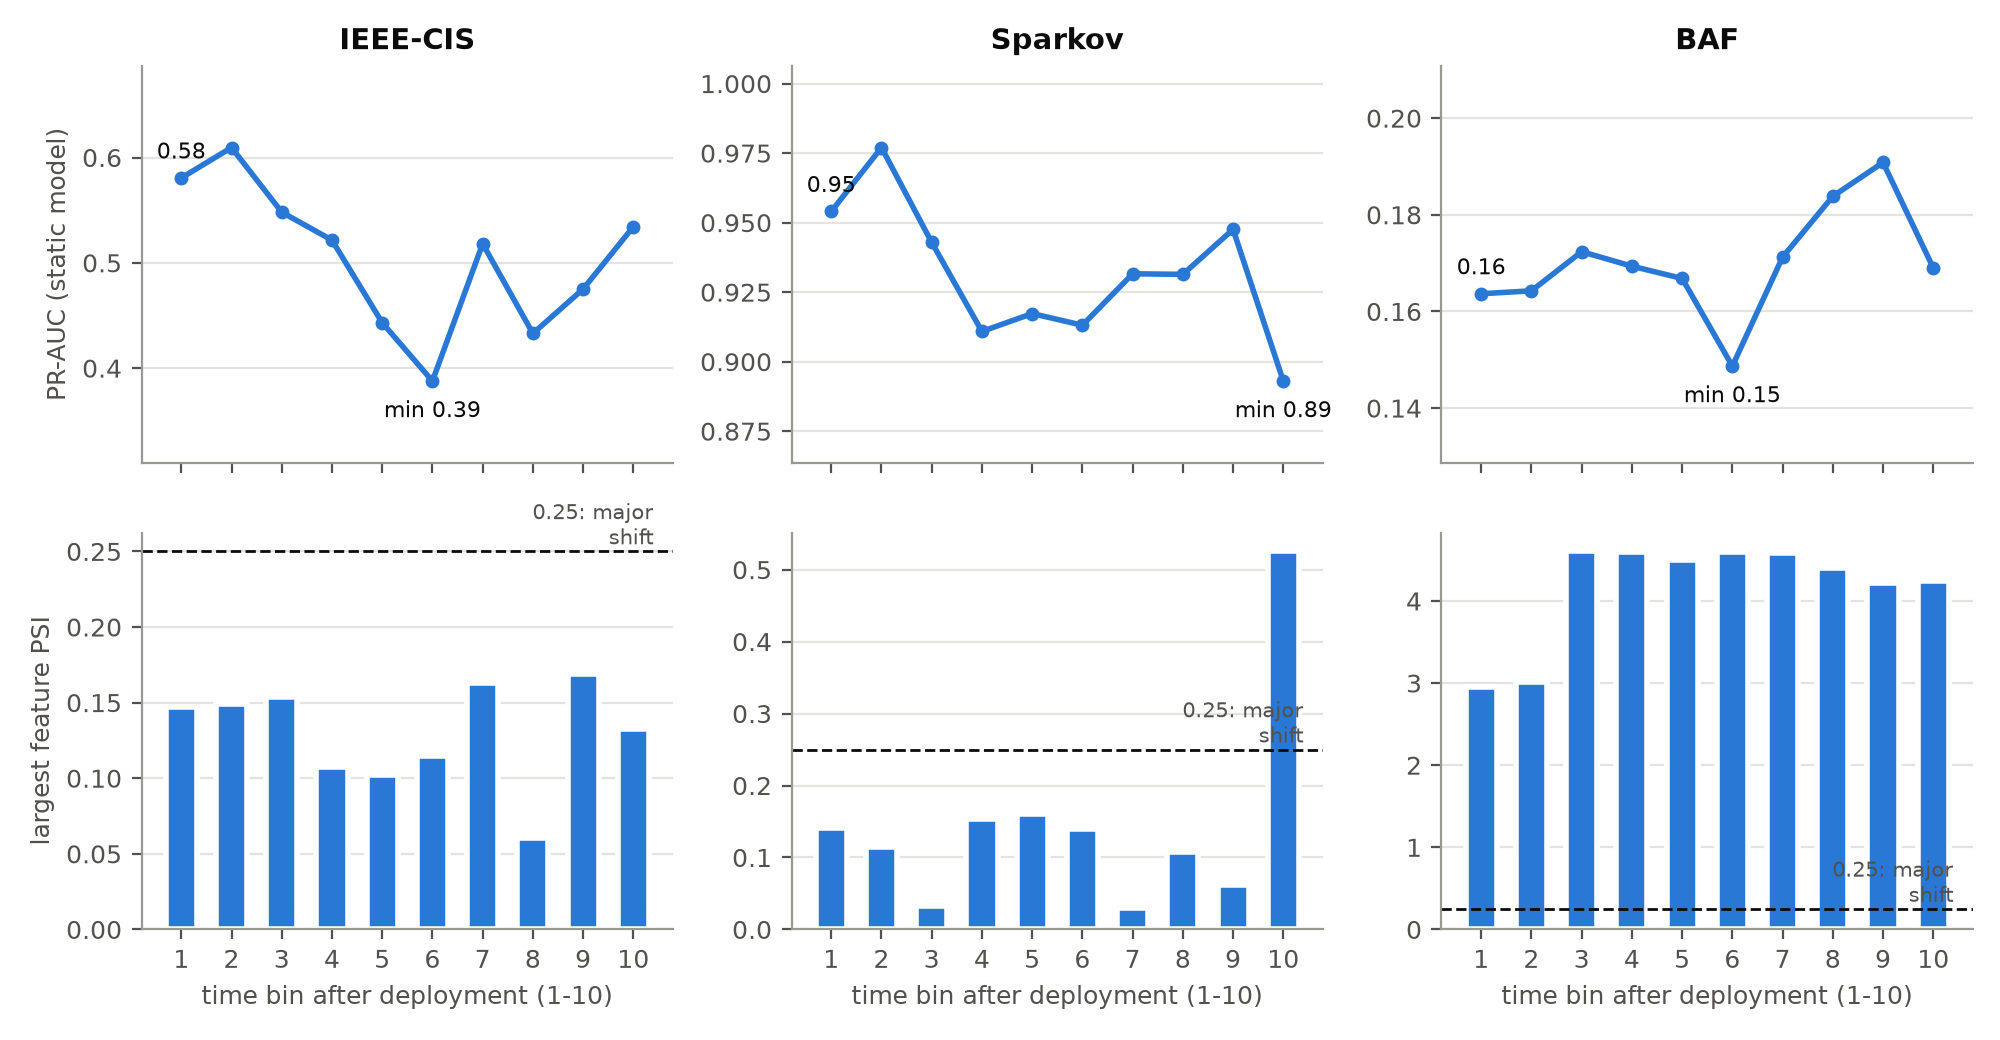
\includegraphics[width=\textwidth]{figures/results_decay.png}
  \caption{Static model after deployment, in ten consecutive time bins of the test period: PR-AUC (top) and the largest PSI among the ten most important features (bottom). Each panel has its own scale}
  \label{fig:decay}
\end{figure}

\textbf{IEEE-CIS decays, and the drift measures do not see it.} The PR-AUC of the static model fell from 0.581 in the first time bin to 0.388 in the sixth, a relative loss of a third, before partly recovering to 0.534. ROC-AUC fell from 0.920 to 0.849 over the same bins. Over the same period, none of the ten most important features reached the 0.25 level of a major shift (the largest PSI was 0.17), and the PSI of the model's scores never exceeded 0.017. A label-free monitor would therefore have reported a stable system during the largest loss of performance in the study. This agrees with the decay that Menezes and Filho observed for graph models on the same dataset \cite{menezes2025}, and shows that the decay is not visible in the input distribution.

\textbf{Sparkov and BAF drift, and the model does not decay.} On Sparkov the per-card activity features drifted strongly in the last bin (PSI 0.53), and on BAF the velocity features shifted far beyond any usual threshold in every bin (PSI up to 4.60), yet PR-AUC stayed within 0.89 to 0.98 on Sparkov and within 0.15 to 0.19 on BAF, without a downward trend. A drift monitor on these features would have raised an alarm in almost every week. The score-PSI trigger, which looks at the model's outputs rather than its inputs, fired only once on Sparkov, at one of the four label delays, and never on BAF.

\textbf{Answer to RQ1.} The performance of a deployed fraud model can decay substantially, but whether it does depends on the data, and label-free drift measures are not a reliable indicator of it in either direction: they missed real decay on IEEE-CIS and signalled drift that did not matter on Sparkov and BAF. This is the situation that Shakil et al. anticipated when they noted that statistical drift does not always mean lower performance \cite{shakil2025}, now observed on natural drift in fraud data.

\subsection{Retraining under Label Delay}\label{sec:rq2}

Table \ref{tab:sweep} and Figure \ref{fig:delaygain} compare scheduled retraining every 14 days with the static model at label delays of 0, 15, 30 and 60 days.

{\footnotesize
\begin{longtable}{>{\raggedright\arraybackslash}p{0.12\textwidth}>{\raggedright\arraybackslash}p{0.09\textwidth}>{\raggedright\arraybackslash}p{0.12\textwidth}>{\raggedright\arraybackslash}p{0.21\textwidth}>{\raggedright\arraybackslash}p{0.21\textwidth}>{\raggedright\arraybackslash}p{0.19\textwidth}}
\caption{Gain in mean weekly PR-AUC over the static model by label delay (retraining every 14 days; 95\% intervals; bold: interval excludes zero)}\label{tab:sweep}\\
\toprule
\textbf{Dataset} & \textbf{Delay} & \textbf{Static} & \textbf{All history} & \textbf{Last 60 days} & \textbf{Drift: performance} \\
\midrule
\endfirsthead
\toprule
\textbf{Dataset} & \textbf{Delay} & \textbf{Static} & \textbf{All history} & \textbf{Last 60 days} & \textbf{Drift: performance} \\
\midrule
\endhead
IEEE-CIS & 0 d & 0.507 & \textbf{+0.033} [0.027, 0.040] & \textbf{+0.078} [0.067, 0.088] & +0.030 (2 retrains) \\ \midrule
 & 15 d & 0.491 & \textbf{+0.025} [0.020, 0.029] & \textbf{+0.062} [0.052, 0.072] & +0.020 (2) \\ \midrule
 & 30 d & 0.474 & \textbf{+0.028} [0.022, 0.033] & \textbf{+0.056} [0.046, 0.064] & +0.027 (3) \\ \midrule
 & 60 d & 0.472 & \textbf{+0.008} [0.002, 0.014] & \textbf{+0.010} [0.004, 0.016] & +0.010 (4) \\ \midrule
Sparkov & 0 d & 0.931 & \textbf{+0.016} [0.013, 0.020] & \textbf{-0.258} [-0.273, -0.242] & 0.000 (0) \\ \midrule
 & 15 d & 0.928 & \textbf{+0.017} [0.013, 0.021] & \textbf{-0.214} [-0.228, -0.199] & 0.000 (0) \\ \midrule
 & 30 d & 0.924 & \textbf{+0.019} [0.016, 0.023] & \textbf{-0.173} [-0.187, -0.160] & 0.000 (0) \\ \midrule
 & 60 d & 0.923 & \textbf{+0.019} [0.015, 0.023] & \textbf{-0.198} [-0.211, -0.183] & 0.000 (0) \\ \midrule
BAF & 0 d & 0.162 & \textbf{+0.011} [0.007, 0.015] & -0.003 [-0.007, 0.002] & 0.000 (0) \\ \midrule
 & 15 d & 0.161 & \textbf{+0.008} [0.004, 0.012] & -0.005 [-0.011, 0.000] & 0.000 (0) \\ \midrule
 & 30 d & 0.161 & \textbf{+0.009} [0.004, 0.014] & \textbf{-0.007} [-0.013, -0.002] & 0.000 (0) \\ \midrule
 & 60 d & 0.155 & \textbf{+0.010} [0.006, 0.015] & +0.002 [-0.003, 0.007] & +0.001 (1) \\ \bottomrule
\end{longtable}
}

\begin{figure}[htbp]
  \centering
  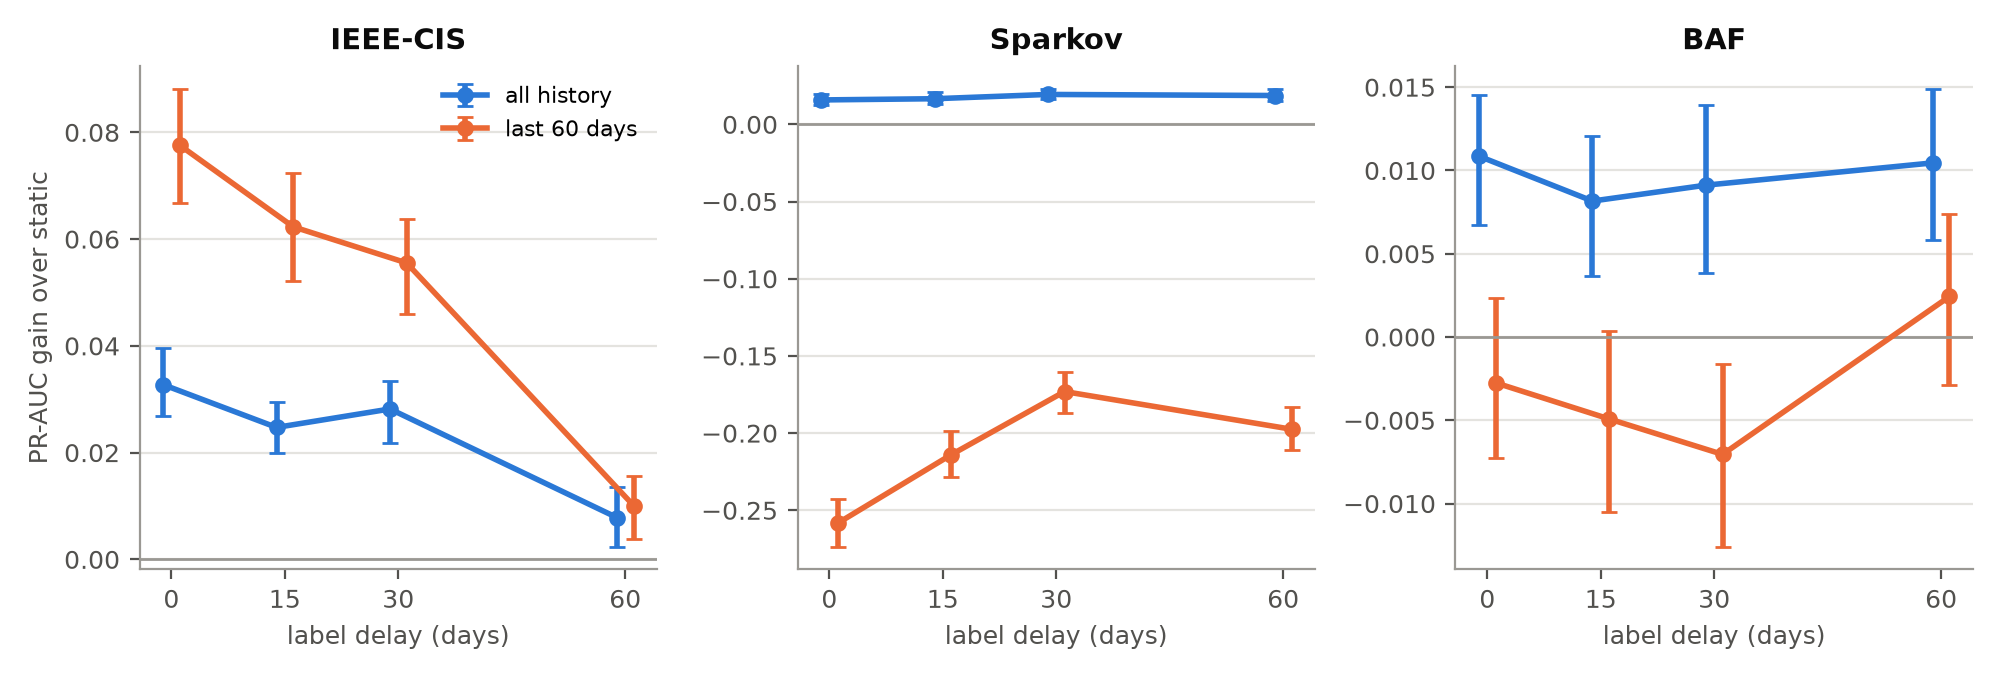
\includegraphics[width=\textwidth]{figures/results_delay.png}
  \caption{Gain in mean weekly PR-AUC over the static model for scheduled retraining every 14 days, by label delay, with 95\% paired bootstrap intervals}
  \label{fig:delaygain}
\end{figure}

\textbf{Retraining helps when its window suits the data.} On IEEE-CIS both windows improved on the static model at every delay, and the last 60 days was clearly better than all history (+0.078 against +0.033 at no delay). On Sparkov and BAF the order reversed: retraining on all history gained +0.016 to +0.019 and +0.008 to +0.011 at every delay, with every interval excluding zero, while the 60-day window was \textit{worse} than not retraining at all, dramatically so on Sparkov (-0.17 to -0.26). Sparkov has only 0.53\% fraud and a stable fraud pattern: 60 days contain too few frauds to learn it again, and the model gains nothing from forgetting older data. IEEE-CIS, in contrast, drifts, and older data teaches the model patterns that no longer hold.

\textbf{Label delay erodes the benefit.} On IEEE-CIS the gain of the 60-day window fell from +0.078 with immediate labels to +0.062 at 15 days, +0.056 at 30 days and +0.010 at 60 days, while the static model itself declined only from 0.507 to 0.472. With 60 days of delay, a retrained model learns from data that is already two months old, which on a drifting dataset is little better than the original training data. On Sparkov and BAF the gain of all-history retraining hardly changed with the delay, which is consistent with their lack of decay: when the pattern is stable, old labels are still useful.

\textbf{Untuned drift triggers rarely act.} With default settings, the performance trigger retrained two to four times on IEEE-CIS and reached between a third and half of the gain of the 60-day schedule at delays up to 30 days. On Sparkov and BAF it almost never fired, because performance never dropped by 15\%, and it behaved like the static model.

\textbf{Answer to RQ2.} Retraining improved performance on every dataset, but only with a training window that suited the data, and on the drifting dataset its benefit shrank sharply as labels arrived later; at 60 days of delay most of the benefit was gone. This confirms, on public data, the importance of verification latency stressed by Dal Pozzolo et al. \cite{dalpozzolo2018}.

\section{Analyse Design Solutions}\label{sec:analyse}

\subsection{Drift-Triggered versus Scheduled Retraining}\label{sec:rq3}

The comparison in Section \ref{sec:rq2} used default settings. Table \ref{tab:walkforward} gives the fair comparison: every family was re-tuned every four weeks with walk-forward tuning over 190 configurations, using only labels that had matured at the time.

{\footnotesize
\begin{longtable}{>{\raggedright\arraybackslash}p{0.12\textwidth}>{\raggedright\arraybackslash}p{0.08\textwidth}>{\raggedright\arraybackslash}p{0.12\textwidth}>{\raggedright\arraybackslash}p{0.16\textwidth}>{\raggedright\arraybackslash}p{0.23\textwidth}>{\raggedright\arraybackslash}p{0.22\textwidth}}
\caption{Walk-forward tuning: each family re-tuned every four weeks on matured labels only (mean weekly PR-AUC, total retrains, and differences with 95\% intervals)}\label{tab:walkforward}\\
\toprule
\textbf{Dataset} & \textbf{Delay} & \textbf{Static} & \textbf{Schedule (retrains)} & \textbf{Schedule - static} & \textbf{Drift trigger - schedule} \\
\midrule
\endfirsthead
\toprule
\textbf{Dataset} & \textbf{Delay} & \textbf{Static} & \textbf{Schedule (retrains)} & \textbf{Schedule - static} & \textbf{Drift trigger - schedule} \\
\midrule
\endhead
IEEE-CIS & 0 d & 0.470 & 0.614 (12) & \textbf{+0.144} [0.132, 0.158] & \textbf{-0.069} [-0.082, -0.060] \\ \midrule
 & 15 d & 0.468 & 0.547 (12) & \textbf{+0.079} [0.070, 0.091] & \textbf{-0.034} [-0.044, -0.027] \\ \midrule
 & 30 d & 0.458 & 0.518 (6) & \textbf{+0.059} [0.049, 0.069] & \textbf{-0.032} [-0.038, -0.025] \\ \midrule
Sparkov & 0 d & 0.916 & 0.945 (12) & \textbf{+0.029} [0.024, 0.033] & -0.001 [-0.003, 0.001] \\ \midrule
 & 15 d & 0.913 & 0.944 (12) & \textbf{+0.031} [0.026, 0.036] & \textbf{-0.007} [-0.010, -0.004] \\ \midrule
 & 30 d & 0.917 & 0.943 (12) & \textbf{+0.027} [0.023, 0.031] & \textbf{-0.007} [-0.009, -0.004] \\ \midrule
BAF & 0 d & 0.163 & 0.174 (8) & \textbf{+0.011} [0.006, 0.016] & \textbf{-0.011} [-0.016, -0.006] \\ \midrule
 & 15 d & 0.157 & 0.168 (8) & \textbf{+0.011} [0.007, 0.016] & \textbf{-0.006} [-0.011, -0.002] \\ \midrule
 & 30 d & 0.159 & 0.162 (7) & +0.003 [-0.003, 0.008] & +0.001 [-0.003, 0.006] \\ \bottomrule
\end{longtable}
}

\textbf{The tuned schedule beat or matched the tuned trigger everywhere.} On IEEE-CIS the schedule was better than the drift trigger by 0.069, 0.034 and 0.032 PR-AUC at delays of 0, 15 and 30 days, all reliable. On Sparkov the trigger came close with far fewer retrains (2 to 8 against 12): the gap was within noise with immediate labels and 0.007 at 15 and 30 days. On BAF the schedule was better at 0 and 15 days, and at 30 days neither retraining family was reliably better than the static model, because the gains on BAF are small. Of the nine comparisons, the trigger was reliably worse in seven and never reliably better.

The reason is visible in how the tuned trigger behaves under label delay. It can only react to a drop in performance after the drop has been confirmed by labels that are at least one delay old, and a drop must exceed noise in weekly PR-AUC before it is acted upon. A schedule keeps the model fresh without waiting for evidence. Where the trigger came close, as on Sparkov, it did so by retraining rarely on a stable dataset where retraining matters little.

\textbf{Answer to RQ3.} No. When both are tuned fairly and labels arrive late, drift-triggered retraining did not outperform scheduled retraining on any of the three datasets; it was worse in most comparisons and at best equal, although it retrained less often. This contradicts the results of Wong and Perumal \cite{wong2025} and Yelleti \cite{yelleti2025}, which were obtained with injected drift or immediate labels. A stronger effect than the choice of trigger was the choice of training window, which changed the result by up to 0.26 PR-AUC.

\subsection{Equal-Budget Comparison}\label{sec:budget}

Scheduled retraining retrained more often than the drift triggers in the comparisons above (for example 12 against 2 to 5 retrains in walk-forward tuning on IEEE-CIS), so part of its advantage could come simply from retraining more often. To separate the two, both families were run over many settings on IEEE-CIS and BAF, schedules every 7 days or more and 64 trigger settings, and every trigger setting was paired with the schedule that uses the same training window and the largest number of retrains that does not exceed the trigger's. The schedule therefore never has more retrains than the trigger it is compared with, which favours the trigger. Table \ref{tab:budget} summarises the pairs and Figure \ref{fig:budget} shows the best PR-AUC each family reaches within a given budget.

{\footnotesize
\begin{longtable}{>{\raggedright\arraybackslash}p{0.11\textwidth}>{\raggedright\arraybackslash}p{0.08\textwidth}>{\raggedright\arraybackslash}p{0.14\textwidth}>{\raggedright\arraybackslash}p{0.08\textwidth}>{\raggedright\arraybackslash}p{0.16\textwidth}>{\raggedright\arraybackslash}p{0.14\textwidth}>{\raggedright\arraybackslash}p{0.10\textwidth}>{\raggedright\arraybackslash}p{0.13\textwidth}}
\caption{Equal-budget comparison: each trigger setting paired with the schedule that uses the same window and no more retrains (95\% intervals; retrains: trigger / schedule)}\label{tab:budget}\\
\toprule
\textbf{Dataset} & \textbf{Delay} & \textbf{Window} & \textbf{Pairs} & \textbf{Schedule better (reliably)} & \textbf{Trigger reliably better} & \textbf{Mean diff.} & \textbf{Retrains} \\
\midrule
\endfirsthead
\toprule
\textbf{Dataset} & \textbf{Delay} & \textbf{Window} & \textbf{Pairs} & \textbf{Schedule better (reliably)} & \textbf{Trigger reliably better} & \textbf{Mean diff.} & \textbf{Retrains} \\
\midrule
\endhead
IEEE-CIS & 0 d & last 60 days & 27 & 18 (9) & 0 & +0.016 & 1.7 / 1.7 \\ \midrule
 & 30 d & last 60 days & 30 & 23 (7) & 0 & +0.011 & 2.2 / 2.2 \\ \midrule
 & 0 d & all history & 28 & 15 (14) & 0 & +0.005 & 1.7 / 1.6 \\ \midrule
 & 30 d & all history & 30 & 12 (0) & 0 & 0.000 & 2.3 / 2.2 \\ \midrule
BAF & 0 d & last 60 days & 9 & 9 (2) & 0 & +0.003 & 2.2 / 2.2 \\ \midrule
 & 30 d & last 60 days & 0 & - & - & - & trigger never fired \\ \midrule
 & 0 d & all history & 10 & 2 (1) & 3 & -0.002 & 1.9 / 1.9 \\ \midrule
 & 30 d & all history & 2 & 2 (1) & 0 & +0.004 & 2.5 / 2.5 \\ \bottomrule
\end{longtable}
}

\begin{figure}[htbp]
  \centering
  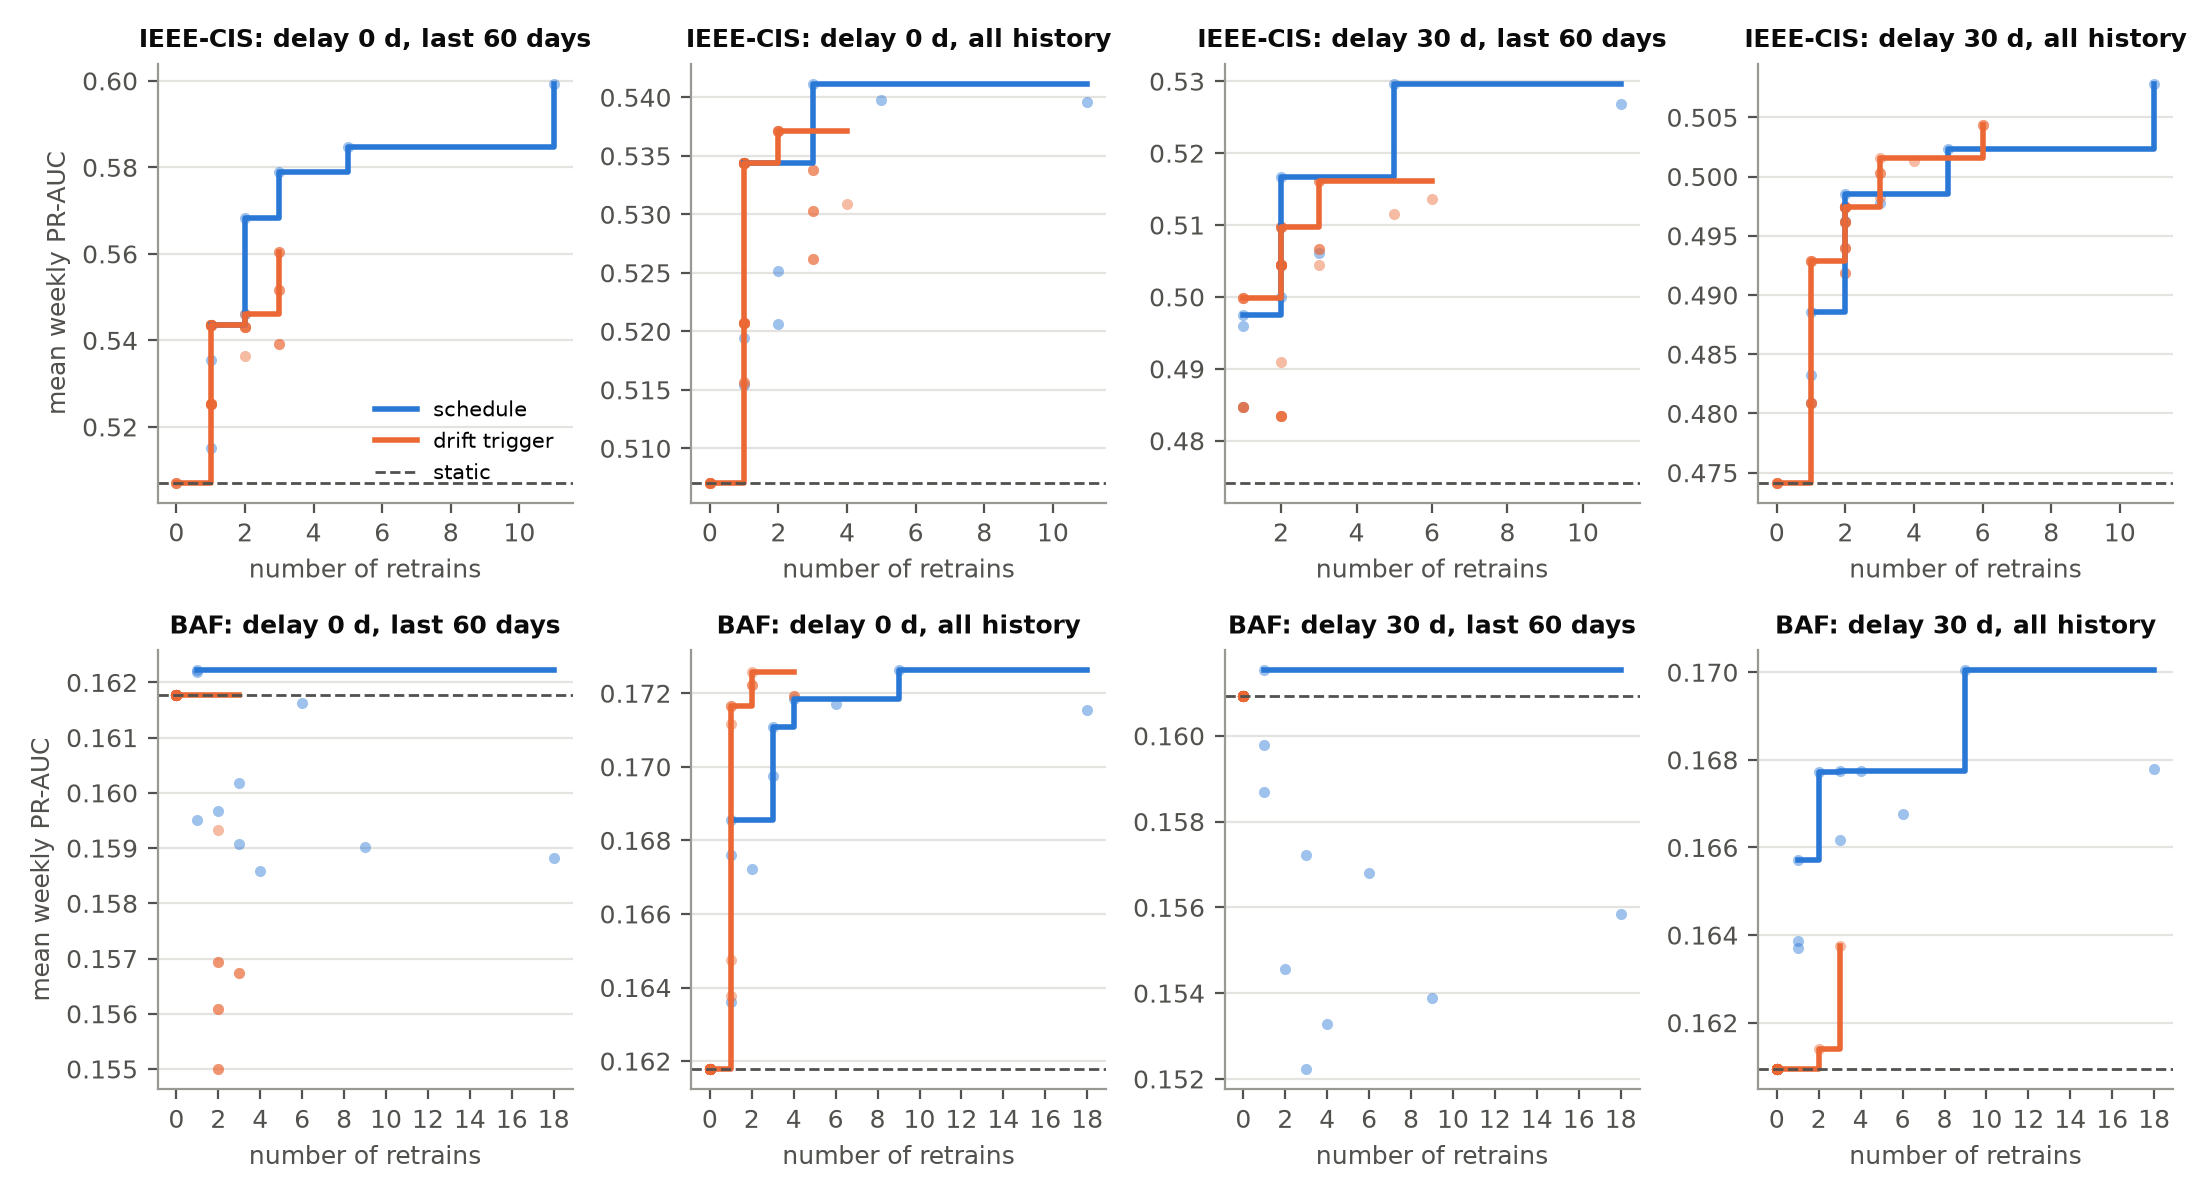
\includegraphics[width=\textwidth]{figures/results_equal_budget.png}
  \caption{Equal-budget comparison on IEEE-CIS (top) and BAF (bottom): the best mean weekly PR-AUC each family reaches with at most a given number of retrains (dots: individual settings)}
  \label{fig:budget}
\end{figure}

With the 60-day window, the best window on IEEE-CIS, the schedule was better in 18 of 27 pairs with immediate labels and 23 of 30 pairs at a 30-day delay, reliably so in 9 and 7 pairs, and the trigger was never reliably better; on average the schedule was 0.016 and 0.011 PR-AUC ahead at the same budget. With two retrains, for example, the best schedule reached 0.568 and the best trigger 0.546. With all history as training data the two were close: the schedule was ahead by 0.005 with immediate labels and level at a 30-day delay. The label-free score-PSI trigger fired only once across all its settings. Finally, the triggers rarely used more than two or three retrains, while the schedule kept improving as it retrained more often (0.599 with eleven retrains).

On BAF the triggers rarely fired at all, because performance hardly changed: most settings never retrained, and at a 30-day delay no setting with the 60-day window fired. Where pairs exist, the picture depends on the label delay. With immediate labels and all history as training data, the trigger was the more economical policy: it was reliably better in 3 of 10 pairs, and its best setting reached 0.173 with two retrains, which the schedule matched only with nine. With the 60-day window the schedule was better in all 9 pairs. At a realistic 30-day delay the schedule was ahead again: with two retrains it reached 0.168 against 0.161 for the best trigger, and 0.170 against 0.164 at best.

The advantage of scheduled retraining is therefore not only a matter of retraining more often. When labels were delayed by 30 days, the schedule matched or beat the drift trigger at an equal budget on both datasets, and it was never reliably worse on IEEE-CIS. A trigger can be economical when labels arrive immediately, as on BAF with all history, which is consistent with earlier work that assumed immediate labels \cite{yelleti2025}; under label delay it has to wait for evidence of degradation and loses that advantage. Part of the schedule's overall advantage also comes from the larger number of retrains, which a delayed-label trigger cannot match. The comparison on Sparkov is being run in the same way.

\subsection{Framework Replay}\label{sec:replay5}

\textbf{Replay.} Table \ref{tab:replay} reports the framework replayed over the stream of each dataset at a 30-day label delay, with four window settings run on the same Kaggle machine. The framework reproduced the offline simulation of the same policy closely: 0.529 against 0.530 for the 60-day window on IEEE-CIS, 0.942 against 0.943 for all history on Sparkov, and 0.169 against 0.170 on BAF. An earlier replay of the default configuration on a desktop computer gave 0.531 on IEEE-CIS. The MLOps components, from the registry and promotion gate to the monitoring loop, therefore add their safeguards without changing the performance of the policy they run.

{\footnotesize
\begin{longtable}{>{\raggedright\arraybackslash}p{0.21\textwidth}>{\raggedright\arraybackslash}p{0.24\textwidth}>{\raggedright\arraybackslash}p{0.24\textwidth}>{\raggedright\arraybackslash}p{0.24\textwidth}}
\caption{Framework replays at a 30-day label delay: mean weekly PR-AUC (retrains, rejected by the gate) and the offline simulation of the same policy}\label{tab:replay}\\
\toprule
\textbf{} & \textbf{IEEE-CIS (12 weeks)} & \textbf{Sparkov (52 weeks)} & \textbf{BAF (19 weeks)} \\
\midrule
\endfirsthead
\toprule
\textbf{} & \textbf{IEEE-CIS (12 weeks)} & \textbf{Sparkov (52 weeks)} & \textbf{BAF (19 weeks)} \\
\midrule
\endhead
Static model & 0.478 & 0.924 & 0.161 \\ \midrule
Last 60 days & \textbf{0.529} (5, 0) & 0.752 (26, 11) & 0.153 (9, 0) \\ \midrule
All history & 0.504 (6, 0) & \textbf{0.942} (25, 0) & \textbf{0.169} (9, 1) \\ \midrule
Automatic window & \textbf{0.529} (5, 0) & \textbf{0.942} (25, 1) & 0.165 (9, 1) \\ \midrule
Window chosen & 60 days in 5 of 5 & all history in 25 of 25 & all history in 7 of 9 \\ \midrule
Offline simulation: last 60 days / all history & 0.530 / 0.502 & 0.751 / 0.943 & 0.154 / 0.170 \\ \bottomrule
\end{longtable}
}

\subsection{Safeguards under Fault Injection}\label{sec:faults5}

\textbf{Safeguards under fault injection.} Table \ref{tab:gatefaults} and Figure \ref{fig:gate} show the IEEE-CIS replay with two faulty retraining jobs. With the promotion gate on, all six faulty models produced by training-job faults were rejected. Shuffled labels gave models with a PR-AUC of 0.035, no better than chance, and the label outage gave 0.275 and 0.445 against champions of 0.475 and 0.620. The feature unit bug was the hardest case: its models scored 0.464 and 0.597 against 0.475 and 0.620, and were rejected only because they were re-scored on production features and fell just beyond the tolerance of 0.01. With the gate on, each of these three faults cost 0.012 PR-AUC, the price of keeping an older champion for two weeks. Without the gate the faulty models were promoted and the cost rose to 0.019, 0.039 and 0.080.

{\footnotesize
\begin{longtable}{>{\raggedright\arraybackslash}p{0.23\textwidth}>{\raggedright\arraybackslash}p{0.10\textwidth}>{\raggedright\arraybackslash}p{0.14\textwidth}>{\raggedright\arraybackslash}p{0.15\textwidth}>{\raggedright\arraybackslash}p{0.32\textwidth}}
\caption{Fault injection on IEEE-CIS (two faulty retraining jobs, 30-day label delay)}\label{tab:gatefaults}\\
\toprule
\textbf{Fault} & \textbf{Gate} & \textbf{Mean PR-AUC} & \textbf{Change vs clean} & \textbf{Faulty models promoted} \\
\midrule
\endfirsthead
\toprule
\textbf{Fault} & \textbf{Gate} & \textbf{Mean PR-AUC} & \textbf{Change vs clean} & \textbf{Faulty models promoted} \\
\midrule
\endhead
None (clean) & on & 0.531 & - & - \\ \midrule
Label shuffle & on & 0.519 & -0.012 & 0 of 2 (0.035 vs 0.475; 0.034 vs 0.620) \\ \midrule
 & off & 0.451 & -0.080 & 2 of 2 \\ \midrule
Label loss (80\%) & on & 0.519 & -0.012 & 0 of 2 (0.275 vs 0.475; 0.445 vs 0.620) \\ \midrule
 & off & 0.492 & -0.039 & 2 of 2 \\ \midrule
Feature unit bug & on & 0.519 & -0.012 & 0 of 2 (0.464 vs 0.475; 0.597 vs 0.620) \\ \midrule
 & off & 0.512 & -0.019 & 2 of 2 \\ \midrule
Upstream label shuffle & on & 0.451 & -0.080 & 2 of 2; safety net replaced each after 7 days \\ \midrule
 & off & 0.451 & -0.080 & 2 of 2 \\ \bottomrule
\end{longtable}
}

\begin{figure}[htbp]
  \centering
  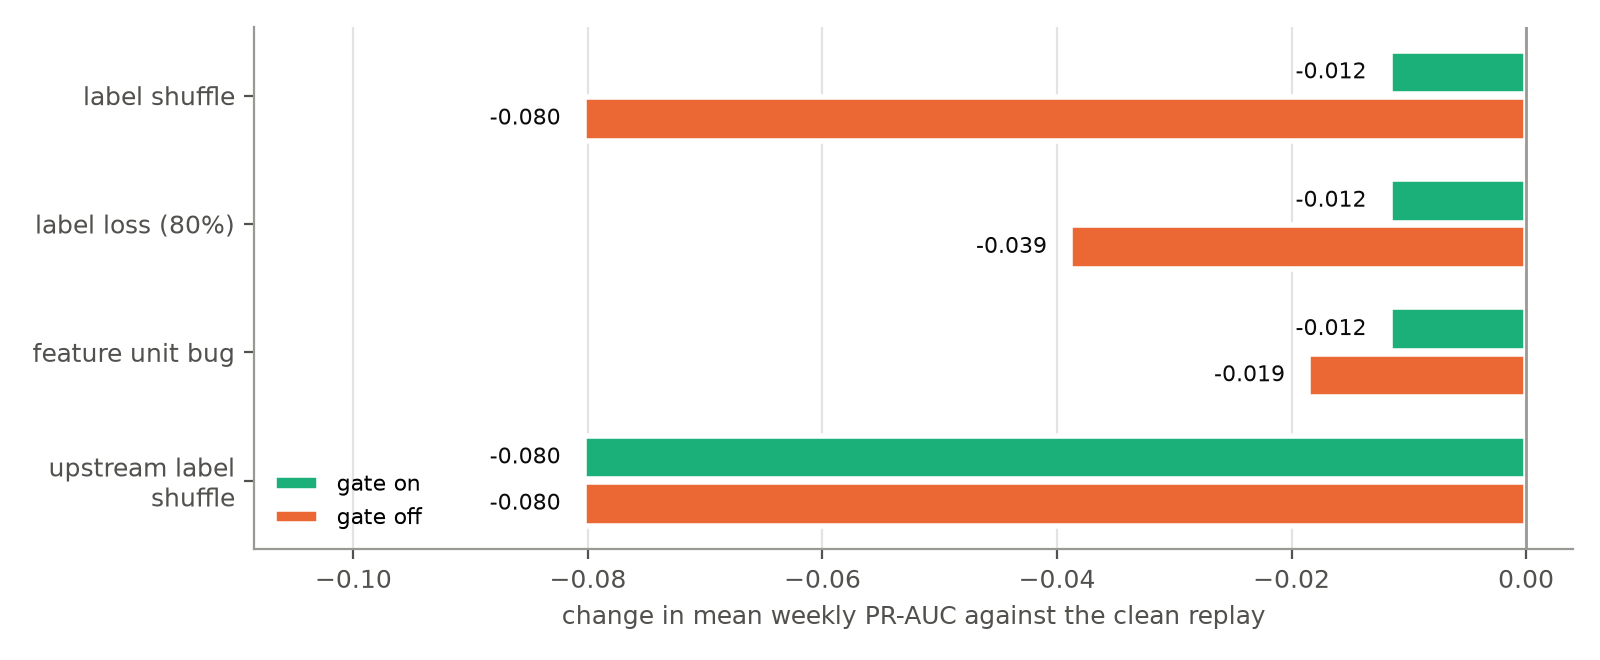
\includegraphics[width=\textwidth]{figures/results_gate.png}
  \caption{Fault injection on IEEE-CIS: change in mean weekly PR-AUC against a clean replay when two retraining jobs are faulty, with the promotion gate on and off}
  \label{fig:gate}
\end{figure}

The upstream fault, which corrupts the label store that the gate itself reads, passed the gate as expected, since both models looked equally poor on corrupted labels. Here the safety net took over: seven days after each faulty promotion, the live PR-AUC on matured labels had fallen to 0.045 and 0.036, below both 70\% of the reference and three times the fraud rate, and the framework retrained early. The damage was limited to one week per fault (-0.080 in total). Before the reference of the safety net included recent live performance (Section \ref{sec:safety}), the same fault went undetected and cost -0.149.

\textbf{Answer to RQ4.} Yes. Built on the findings of RQ1 to RQ3, the framework sustained the performance of the best offline policy in a full replay, prevented every faulty model it could observe from reaching production, recovered within a week from the fault it could not observe, and, with automatic window selection, performed at or near the best fixed window on all three datasets.

\section{Final Design Adjustments}\label{sec:adjust}

Three changes were made to the design during the evaluation, each prompted by a result.

\subsection{Promotion Gate on Production Features}\label{sec:adj_gate}

The first version of the promotion gate compared the challenger and the champion using scores stored when each model was trained. A fault test with a feature unit bug showed the weakness of this: a model trained on wrongly scaled features looks good on equally wrong validation data. The gate was changed to re-score both models through the production feature path (Section \ref{sec:gate}), after which it rejected the faulty models.

\subsection{Safety-Net Reference from Live Performance}\label{sec:adj_safety}

Originally the safety net compared live PR-AUC with the model's own validation PR-AUC. When the label store itself was corrupted, a faulty model reported a poor validation score and was then judged against that low bar, so the fault went undetected and cost 0.149 PR-AUC. The reference was changed to the better of the validation score and the median of the last four live measurements, and a no-skill check was added (Section \ref{sec:safety}); the same fault was then caught after seven days and cost 0.080.

\subsection{Automatic Training-Window Selection}\label{sec:adj_window}

\textbf{Automatic window selection.} No fixed window suited all three datasets: the 60-day window was best on IEEE-CIS (0.529) but lost 0.172 against the static model on Sparkov, while all history was best on Sparkov and BAF but only second on IEEE-CIS. With automatic selection, the framework chose the 60-day window at all five retrains on IEEE-CIS and all history at all 25 retrains on Sparkov, matching the best fixed window on both (difference 0.000 and -0.0002). On BAF it chose the 60-day window at the first two retrains, when the two candidates were close and the shorter window scored slightly higher on recent data, and all history at the remaining seven. It ended 0.0045 below the best fixed window on BAF, a small but reliable difference (95\% interval over weeks -0.008 to -0.001), and 0.004 above the static model. Figure \ref{fig:window} shows that the automatic setting avoided the large loss of a wrongly chosen window on every dataset without knowing in advance which window suited the data.

\begin{figure}[htbp]
  \centering
  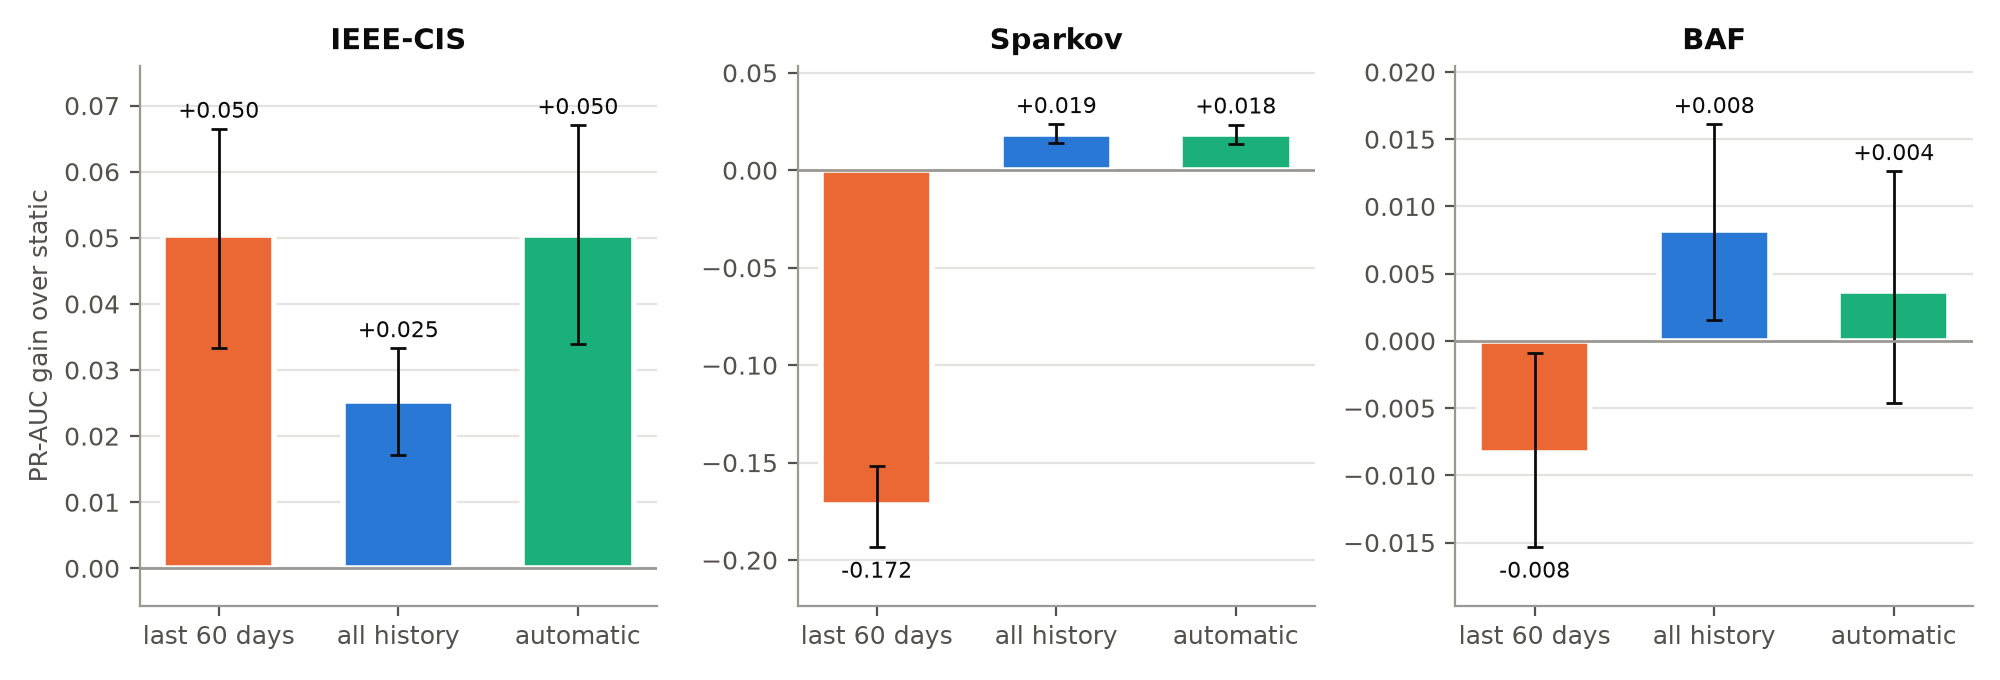
\includegraphics[width=\textwidth]{figures/results_window.png}
  \caption{Framework replays (30-day label delay): gain in mean weekly PR-AUC over the static model for each training-window choice, with 95\% bootstrap intervals over weeks}
  \label{fig:window}
\end{figure}

\section{Summary of Results}\label{sec:summary}

Table \ref{tab:answers} summarises the answers to the research questions. Taken together, the results support the design of the proposed framework: performance is monitored on delayed labels rather than inferred from drift, retraining follows a schedule rather than a drift alarm, the training window is selected from the data, and every new model must pass a promotion gate. Section \ref{sec:discussion} discusses what these results mean, how they relate to earlier work, and where they are limited.

{\footnotesize
\begin{longtable}{>{\raggedright\arraybackslash}p{0.09\textwidth}>{\raggedright\arraybackslash}p{0.85\textwidth}}
\caption{Answers to the research questions}\label{tab:answers}\\
\toprule
\textbf{RQ} & \textbf{Answer} \\
\midrule
\endfirsthead
\toprule
\textbf{RQ} & \textbf{Answer} \\
\midrule
\endhead
RQ1 & Performance after deployment changed differently on each dataset: it fell by a third on IEEE-CIS but stayed stable on Sparkov and BAF. Label-free drift measures did not reflect this: input and score drift stayed low while IEEE-CIS decayed, and input drift was strong (PSI up to 4.6) while Sparkov and BAF did not. \\ \midrule
RQ2 & Scheduled retraining improved performance on every dataset when its window suited the data, with gains of 0.008 to 0.078 PR-AUC. On IEEE-CIS the gain shrank from 0.078 to 0.010 as the label delay grew from 0 to 60 days. \\ \midrule
RQ3 & No. Tuned fairly with walk-forward tuning, drift-triggered retraining was worse than scheduled retraining in 7 of 9 comparisons and never better beyond noise; it retrained less often. The training window mattered more than the trigger. \\ \midrule
RQ4 & Yes. The framework reproduced the offline results within 0.002 PR-AUC, blocked every faulty model the gate could observe, limited the damage of the unobservable fault through the safety net, and, with automatic window selection, matched the best fixed window on two datasets and came within 0.005 on the third. \\ \bottomrule
\end{longtable}
}

\section{Statistical Analysis}\label{sec:statistics}

Three layers of statistical analysis support the results. First, every comparison between strategies is paired: all strategies are evaluated on the same weeks and the same bootstrap resamples, which removes most of the noise they share. Second, the paired day-block bootstrap resamples whole days within each week, which respects the correlation between transactions of the same day, and yields the 95\% intervals reported throughout. Third, training randomness is covered by repeating the key comparisons with five LightGBM seeds.

{\footnotesize
\begin{longtable}{>{\raggedright\arraybackslash}p{0.12\textwidth}>{\raggedright\arraybackslash}p{0.08\textwidth}>{\raggedright\arraybackslash}p{0.24\textwidth}>{\raggedright\arraybackslash}p{0.24\textwidth}>{\raggedright\arraybackslash}p{0.24\textwidth}}
\caption{Key differences over five training seeds (mean, and the number of seeds in which the difference is positive). Best schedule: last 60 days on IEEE-CIS, all history on Sparkov and BAF}\label{tab:seeds}\\
\toprule
\textbf{Dataset} & \textbf{Delay} & \textbf{All history - static} & \textbf{Last 60 days - static} & \textbf{Default drift trigger - best schedule} \\
\midrule
\endfirsthead
\toprule
\textbf{Dataset} & \textbf{Delay} & \textbf{All history - static} & \textbf{Last 60 days - static} & \textbf{Default drift trigger - best schedule} \\
\midrule
\endhead
IEEE-CIS & 0 d & +0.033 (5/5) & +0.080 (5/5) & -0.055 (0/5) \\ \midrule
 & 30 d & +0.022 (5/5) & +0.046 (5/5) & -0.026 (0/5) \\ \midrule
Sparkov & 0 d & +0.012 (5/5) & -0.194 (0/5) & -0.012 (0/5) \\ \midrule
 & 30 d & +0.016 (5/5) & -0.171 (0/5) & -0.016 (0/5) \\ \midrule
BAF & 0 d & +0.006 (5/5) & -0.006 (0/5) & -0.006 (0/5) \\ \midrule
 & 30 d & +0.009 (5/5) & -0.007 (0/5) & -0.009 (0/5) \\ \bottomrule
\end{longtable}
}

\textbf{The results are not due to training randomness.} Table \ref{tab:seeds} repeats the key comparisons with five LightGBM seeds. Every difference in the table had the same sign in all five seeds on every dataset. The spread of a single configuration across seeds was small compared with the differences between strategies: the median standard deviation was 0.004 on IEEE-CIS, 0.010 on Sparkov and 0.003 on BAF.

Because many comparisons are reported, a single interval that excludes zero should not be over-interpreted. The conclusions of this thesis rest instead on patterns that hold across label delays, datasets, seeds and analyses: for example, the drift trigger was reliably worse than the schedule in seven of nine walk-forward comparisons and never reliably better in any of them, and the equal-budget analysis pointed the same way whenever labels were delayed.

\section{Discussions}\label{sec:discussion}

\textbf{Drift indicators and delayed labels.} The central finding is that label-free drift indicators did not reflect what mattered. They stayed quiet while the IEEE-CIS model lost a third of its PR-AUC, and they signalled strong drift on Sparkov and BAF while the models were unaffected. Shakil et al. noted that statistical drift does not always mean lower performance \cite{shakil2025}; on natural drift in fraud data we observed this in both directions. For a fraud system this means that drift alarms should inform investigation, not trigger retraining, and that the performance on matured labels is the signal to watch, even though it arrives late. This is the sense in which the framework is drift-aware.

\textbf{Schedules and triggers.} Earlier work reported that drift-triggered retraining matches or beats a schedule with fewer retrains \cite{wong2025,yelleti2025}. Those results were obtained with injected drift or immediate labels. Under realistic label delay a performance trigger can only react after a drop has been confirmed on labels that are weeks old, and a label-free trigger reacts to the wrong signal. A schedule needs no evidence and keeps the model fresh, and the equal-budget analysis shows that under label delay its advantage is not merely a matter of retraining more often. With immediate labels, a trigger could be the more economical policy, as on BAF, which explains why earlier studies that assumed immediate labels favoured triggers. The result is consistent with Dal Pozzolo et al., who stressed that verification latency shapes how a fraud model can be updated \cite{dalpozzolo2018}, and with Amekoe et al., who found that batch models retrained on delayed labels remain competitive \cite{amekoe2024}.

\textbf{The training window.} The choice of training window changed results by up to 0.26 PR-AUC, far more than the choice of trigger. Recent data was best on IEEE-CIS, which decays, and all history was best on Sparkov and BAF, which are stable and have few frauds. Because no fixed window suits every deployment, selecting the window from the data, as the framework now does, is a practical way to avoid a costly wrong choice.

\textbf{Safe automation.} Automated retraining will eventually train on bad data. The fault tests show that a promotion gate that re-scores models on production data stops faults it can observe, and that a safety net based on live performance limits the damage of faults it cannot. Closed-loop MLOps frameworks such as HAMF \cite{reda2025} automate the loop; this thesis adds evidence on how such safeguards behave when labels arrive late.

\textbf{Limitations.} The deployment is replayed from historical data, so live latency and the behaviour of a real chargeback feed are not observed, and every label arrives after the same delay, without faster investigator feedback. One model family is used throughout. IEEE-CIS covers only six months, Sparkov is simulated, and BAF records only the month of each application, so drift within a month cannot appear. The equal-budget comparison is complete on IEEE-CIS and BAF and under way on Sparkov, and the scoring service has not yet been load tested.

\chapter{Conclusion}

\section{Summary of Findings}\label{sec:findings}

This thesis set out to design and evaluate a drift-aware continuous learning MLOps framework for financial transaction fraud detection that identifies when a deployed model is becoming outdated, decides when retraining is necessary, and deploys a better model safely. Replaying three public datasets under realistic label delay led to five main findings:

\begin{enumerate}
  \item Label-free drift indicators did not reflect model performance: they missed a loss of a third of the PR-AUC on IEEE-CIS and signalled strong drift on Sparkov and BAF, where performance did not fall.
  \item Retraining improved performance on every dataset when its training window suited the data, but label delay eroded its benefit: on IEEE-CIS the gain fell from +0.078 PR-AUC with immediate labels to +0.010 with a 60-day delay.
  \item Tuned fairly, drift-triggered retraining was never reliably better than a fixed schedule and was reliably worse in seven of nine comparisons; with delayed labels the schedule matched or beat it also at an equal retraining budget, while with immediate labels a trigger could retrain more economically.
  \item The training window mattered more than the trigger, and automatic window selection matched the best fixed window on two datasets and came within 0.005 PR-AUC on the third.
  \item The framework reproduced the offline results in a full replay, its promotion gate blocked every faulty model it could observe, and its safety net limited the damage of the fault it could not observe to one week.
\end{enumerate}

\section{Contributions to the Field}\label{sec:contributions}

\begin{enumerate}
  \item An evaluation of retraining policies for fraud detection on public data in strict time order, with explicit label delay, paired bootstrap intervals, walk-forward tuning, repeated seeds and three datasets.
  \item Evidence, on natural drift, that label-free drift indicators are an unreliable trigger for retraining fraud models, and a definition of drift-awareness based on delayed-label performance instead.
  \item An equal-budget comparison showing that, under label delay, the advantage of scheduled retraining is not only due to retraining more often.
  \item A drift-aware MLOps framework with delayed-label monitoring, a scheduled policy with a safety net, automatic window selection and a promotion gate that re-scores models on production features, tested by fault injection.
  \item Open, reproducible code with resumable experiments and Kaggle notebooks, so that every result can be regenerated from the public datasets.
\end{enumerate}

\section{Recommendations for Future Work}\label{sec:future}

\begin{enumerate}
  \item Complete the equal-budget comparison on Sparkov, and load test the scoring service (throughput and p95/p99 latency at increasing concurrency), as recommended in supervisor feedback.
  \item Model faster investigator feedback alongside delayed chargebacks, which could make performance-based triggers react sooner.
  \item Repeat the study with other model families, such as neural and online learners, to test whether the findings depend on gradient boosted trees.
  \item Monitor the stability of model explanations under drift \cite{john2025,uddin2026} and drift in several data sources separately \cite{hassan2026}.
  \item Deploy the framework on a live transaction stream with real label feeds, for example behind a streaming platform \cite{kaushik2025}.
\end{enumerate}


\clearpage
\addcontentsline{toc}{chapter}{Bibliography}
% IEEE style, numbered in order of first citation
\begin{thebibliography}{99}
\bibitem{uddin2026}
M. N. Uddin and M. M. Aziz, ``Shapley value-guided adaptive ensemble learning for explainable financial fraud detection with U.S. regulatory compliance validation,'' arXiv preprint arXiv:2604.14231, 2026.

\bibitem{dalpozzolo2018}
A. Dal Pozzolo, G. Boracchi, O. Caelen, C. Alippi, and G. Bontempi, ``Credit card fraud detection: A realistic modeling and a novel learning strategy,'' \textit{IEEE Transactions on Neural Networks and Learning Systems}, vol. 29, no. 8, pp. 3784--3797, 2018. doi: 10.1109/TNNLS.2017.2736643.

\bibitem{alessi2026}
G. Alessi and M. Fugini, ``Adaptive real-time financial fraud detection with explainable AI tools,'' \textit{Digital Threats: Research and Practice}, vol. 7, no. 1, pp. 1--31, 2026. doi: 10.1145/3794859.

\bibitem{dang2021}
T. Dang, T. Tran, L. Tuan, and M. Tiep, ``Machine learning based on resampling approaches and deep reinforcement learning for credit card fraud detection systems,'' \textit{Applied Sciences}, vol. 11, no. 21, p. 10004, 2021. doi: 10.3390/app112110004.

\bibitem{abdelnaby2023}
A. Abd El-Naby, E. E.-D. Hemdan, and A. El-Sayed, ``An efficient fraud detection framework with credit card imbalanced data in financial services,'' \textit{Multimedia Tools and Applications}, vol. 82, pp. 4139--4160, 2023. doi: 10.1007/s11042-022-13434-6.

\bibitem{sohony2018}
I. Sohony, R. Pratap, and U. Nambiar, ``Ensemble learning for credit card fraud detection,'' in \textit{Proceedings of the ACM India Joint International Conference on Data Science and Management of Data (CoDS-COMAD)}, 2018, pp. 289--294. doi: 10.1145/3152494.3156815.

\bibitem{mienye2023}
I. D. Mienye and Y. Sun, ``A deep learning ensemble with data resampling for credit card fraud detection,'' \textit{IEEE Access}, vol. 11, pp. 30628--30638, 2023. doi: 10.1109/ACCESS.2023.3262020.

\bibitem{amekoe2024}
K. M. Amekoe, M. Lebbah, G. Jaffre, H. Azzag, and Z. Chelly Dagdia, ``Evaluating the efficacy of instance incremental vs. batch learning in delayed label environments: An empirical study on tabular data streaming for fraud detection,'' arXiv preprint arXiv:2409.10111, 2024. doi: 10.48550/arXiv.2409.10111.

\bibitem{pulicharla2019}
M. R. Pulicharla, ``Detecting and addressing model drift: Automated monitoring and real-time retraining in ML pipelines,'' \textit{World Journal of Advanced Research and Reviews}, vol. 3, no. 2, pp. 147--152, 2019. doi: 10.30574/wjarr.2019.3.2.0189.

\bibitem{kodakandla2024}
N. Kodakandla, ``Data drift detection and mitigation: A comprehensive MLOps approach for real-time systems,'' \textit{International Journal of Science and Research Archive}, vol. 12, no. 1, pp. 3127--3139, 2024. doi: 10.30574/ijsra.2024.12.1.0724.

\bibitem{menezes2025}
R. S. Menezes and R. H. Filho, ``Semantic and structural drift in financial knowledge graphs: A robustness analysis of GNN-based fraud detectors,'' in \textit{2025 IEEE International Conference on Knowledge Graph (ICKG)}, Limassol, Cyprus, 2025, pp. 285--291. doi: 10.1109/ICKG66886.2025.00044.

\bibitem{shakil2025}
M. N. P. Shakil, M. S. Islam, N. Noman, and M. Papini, ``Feature drift-guided adaptive ML retraining: An MLOps approach for big data analytics,'' in \textit{2025 IEEE International Conference on Big Data (BigData)}, Macau, China, 2025, pp. 7719--7727. doi: 10.1109/BigData66926.2025.11401445.

\bibitem{wong2025}
H. M. Wong and S. Perumal, ``AI-driven model-retraining architecture to sustain operational accuracy in data-drifting environments,'' in \textit{2025 IEEE Symposium on Wireless Technology \& Applications (ISWTA)}, Penang, Malaysia, 2025, pp. 1--6. doi: 10.1109/ISWTA68114.2025.11329530.

\bibitem{yelleti2025}
V. Yelleti, ``ROSFD: Robust online streaming fraud detection with resilience to concept drift in data streams,'' arXiv preprint arXiv:2504.10229, 2025.

\bibitem{somasundaram2019}
A. Somasundaram and S. Reddy, ``Parallel and incremental credit card fraud detection model to handle concept drift and data imbalance,'' \textit{Neural Computing and Applications}, vol. 31, pp. 3--14, 2019. doi: 10.1007/s00521-018-3633-8.

\bibitem{aldaoud2025}
K. I. Al-Daoud and I. A. Abu-AlSondos, ``Robust AI for financial fraud detection in the GCC: A hybrid framework for imbalance, drift, and adversarial threats,'' \textit{Journal of Theoretical and Applied Electronic Commerce Research}, vol. 20, no. 2, p. 121, 2025. doi: 10.3390/jtaer20020121.

\bibitem{hassan2026}
Y. Hassan, ``DriftGuard-TriAudit: Concept-drift-aware continual multimodal learning for evolving financial statement fraud detection,'' \textit{Journal of Computing and Electronic Information Management}, vol. 22, no. 1, 2026. doi: 10.54097/5bjxgq31.

\bibitem{reda2025}
A. Reda, S. A. Taie, and M. E. Shaheen, ``Hybrid MLOps framework for automated lifecycle management of adaptive phishing detection models,'' \textit{Scientific Reports}, vol. 15, no. 1, p. 38478, 2025. doi: 10.1038/s41598-025-23600-z.

\bibitem{john2025}
S. John, ``Fair and explainable credit-scoring under concept drift: Adaptive explanation frameworks for evolving populations,'' arXiv preprint arXiv:2511.03807, 2025.

\bibitem{kaushik2025}
S. Kaushik, K. K. Dokka, D. Patel, Z. Mamadiyarov, and B. Matchanova, ``Real-time analytics with intelligent data pipelines and ML detection,'' in \textit{2025 International Conference on Sustainability, Innovation \& Technology (ICSIT)}, Nagpur, India, 2025, pp. 1--7. doi: 10.1109/ICSIT65336.2025.11295098.
\end{thebibliography}

\end{document}
